% ============================================================
%  MÉMOIRE DE FIN D'ÉTUDES -ENSPY / UY1
%  TOMI OLAMA GABRIELLE SOLANGE -21P643
%  Standardisation de l'audit de sécurité -MUSA
% ============================================================
\documentclass[12pt,a4paper,oneside]{report}

\usepackage[utf8]{inputenc}
\usepackage[T1]{fontenc}
\usepackage{mathptmx}
\usepackage{subcaption}
\usepackage{geometry}
\geometry{a4paper,top=3cm,bottom=2.5cm,left=3cm,right=2.5cm,
          headheight=1.6cm,headsep=0.5cm,footskip=1.5cm}

\usepackage{setspace}
\onehalfspacing

% ── Palette : bleu marine profond + or chaud + ardoise ─────
\usepackage[dvipsnames,table]{xcolor}
\definecolor{navy}{RGB}{15,40,80}
\definecolor{gold}{RGB}{196,160,70}
\definecolor{lightgold}{RGB}{230,210,150}
\definecolor{cream}{RGB}{252,249,242}
\definecolor{steel}{RGB}{90,110,140}
\definecolor{lightnavy}{RGB}{220,228,242}
\definecolor{theadcolor}{RGB}{15,40,80}
\definecolor{trow1}{RGB}{235,240,250}
\definecolor{trow2}{RGB}{252,252,255}
\definecolor{chapternum}{RGB}{220,228,242}

% ── TikZ ───────────────────────────────────────────────────
\usepackage{graphicx,float}
\usepackage{tikz}
\usetikzlibrary{calc,shapes.geometric,patterns,
                decorations.pathmorphing,decorations.markings,
                positioning,arrows.meta}
\usepackage{pgfornament}

% ── Maths ──────────────────────────────────────────────────
\usepackage{amsmath,amssymb}

% ── Tableaux ───────────────────────────────────────────────
\usepackage{booktabs,tabularx,longtable,multirow,colortbl,array,makecell}
\usepackage{morefloats}
\extrafloats{100}
\usepackage{caption}
\captionsetup{font=small,labelfont=bf,labelsep=period}
\captionsetup[table]{position=above}
\captionsetup[figure]{position=below}

% ── Texte ──────────────────────────────────────────────────
\usepackage{lettrine}
\usepackage{enumitem}
\usepackage{comment}
\usepackage{pifont}
\usepackage{microtype}
\setlength{\parskip}{5pt}
\setlength{\parindent}{0pt}

% ── Boîtes ─────────────────────────────────────────────────
\usepackage[most]{tcolorbox}
\tcbuselibrary{breakable,skins}

\newtcolorbox{questionbox}{
  enhanced, breakable,
  colback=cream, colframe=navy,
  boxrule=1.2pt, arc=0pt,
  left=10pt, right=10pt, top=10pt, bottom=10pt,
  title={\bfseries Probl\'ematique de recherche},
  coltitle=white, colbacktitle=navy,
  attach boxed title to top left={xshift=6mm,yshift=-3mm},
  boxed title style={sharp corners, boxrule=0pt, arc=0pt}
}

\newtcolorbox{encadre}[1][]{
  enhanced, breakable,
  colback=lightnavy!40, colframe=navy!60,
  boxrule=0.6pt, arc=2pt,
  left=8pt, right=8pt, top=8pt, bottom=8pt,
  #1
}

\newtcolorbox{goldbox}[1][]{
  enhanced, breakable,
  colback=cream, colframe=gold,
  boxrule=1pt, arc=0pt,
  borderline west={3pt}{0pt}{navy},
  left=10pt, right=8pt, top=8pt, bottom=8pt,
  #1
}

% ── Minitoc ────────────────────────────────────────────────
\usepackage{minitoc}
\setcounter{minitocdepth}{2}
\mtcsetrules{minitoc}{on}
\mtcsettitle{minitoc}{\textsc{\color{navy}Sommaire du chapitre}}
\mtcsetfont{minitoc}{section}{\small\normalfont\color{navy}}
\mtcsetfont{minitoc}{subsection}{\scriptsize\normalfont}

% ── Titres de chapitres ────────────────────────────────────
\usepackage{titlesec}
\titleformat{\chapter}[display]
  {\normalfont\bfseries\color{navy}}
  {\filleft
   \begin{tikzpicture}[baseline]
     \node[fill=navy, text=white, font=\Large\bfseries,
           inner sep=8pt, minimum width=2.2cm,
           minimum height=1cm]
       {\thechapter};
     \node[anchor=west, text=gold, font=\small\bfseries,
           xshift=2.5cm, yshift=0.1cm] at (0,0)
       {CHAPITRE};
   \end{tikzpicture}%
  }
  {0pt}
  {\filright\huge\bfseries\color{navy}}
  [\vspace{3pt}{\color{navy}\rule{0.6\textwidth}{2pt}}{\color{gold}\rule{0.4\textwidth}{1pt}}]

\titleformat{\section}
  {\normalfont\large\bfseries\color{navy}}
  {\colorbox{navy}{\color{white}\small\thesection}}{0.7em}{}
\titleformat{\subsection}
  {\normalfont\normalsize\bfseries\color{steel}}
  {\thesubsection}{1em}{}
\titleformat{\subsubsection}
  {\normalfont\normalsize\itshape\bfseries\color{steel!80}}
  {\thesubsubsection}{1em}{}

\titlespacing*{\chapter}{0pt}{-10pt}{20pt}
\titlespacing*{\section}{0pt}{14pt}{6pt}
\titlespacing*{\subsection}{0pt}{10pt}{4pt}

% ── En-têtes / pieds ───────────────────────────────────────
\usepackage{fancyhdr}
\pagestyle{fancy}
\fancyhf{}
\renewcommand{\chaptermark}[1]{\markboth{#1}{}}
\renewcommand{\sectionmark}[1]{\markright{\thesection\ #1}}

\fancyhead[LE]{%
  \small\color{steel}%
  \begin{tikzpicture}[baseline=-3pt]
    \draw[gold, line width=1pt] (0,0) -- (0.3,0);
  \end{tikzpicture}%
  \quad\textit{\leftmark}%
}
\fancyhead[RO]{%
  \small\color{steel}%
  \textit{\rightmark}\quad%
  \begin{tikzpicture}[baseline=-3pt]
    \draw[gold, line width=1pt] (0,0) -- (0.3,0);
  \end{tikzpicture}%
}
\fancyfoot[C]{%
  
\begin{tikzpicture}[baseline=-3pt]
    \node[fill=navy, text=white, font=\small\bfseries,
          inner sep=3pt, minimum width=0.8cm] {\thepage};
  \end{tikzpicture}%
}
\fancyfoot[LO,RE]{\small\color{steel!70}%
  \textit{ENSPY - M\'emoire de fin d'\'etudes  2025-2026}}
\renewcommand{\headrulewidth}{0.4pt}
\renewcommand{\headrule}{\color{navy!30}\hrule width\textwidth height 0.4pt}
\renewcommand{\footrulewidth}{0.4pt}
\renewcommand{\footrule}{\color{gold!60}\hrule width\textwidth height 0.4pt}

\fancypagestyle{plain}{
  \fancyhf{}
  \fancyfoot[C]{%
    
\begin{tikzpicture}[baseline=-3pt]
      \node[fill=navy, text=white, font=\small\bfseries,
            inner sep=3pt, minimum width=0.8cm] {\thepage};
    \end{tikzpicture}%
  }
  \fancyfoot[LO,RE]{\small\color{steel!70}%
    \textit{ENSPY - M\'emoire de fin d'\'etudes 2025-2026}}
  \renewcommand{\headrulewidth}{0pt}
  \renewcommand{\footrulewidth}{0.4pt}
  \renewcommand{\footrule}{\color{gold!60}\hrule width\textwidth height 0.4pt}
}

% ── Liens ──────────────────────────────────────────────────
\usepackage[colorlinks=true,linkcolor=navy,citecolor=steel,
            urlcolor=gold,bookmarks=true,bookmarksnumbered=true]{hyperref}
\usepackage{chngcntr}
\counterwithin{table}{chapter}
\counterwithin{figure}{chapter}

% ============================================================
%  PAGE D'ANNONCE CHAPITRE -design circuit imprimé / blueprint
%  #1 = numéro, #2 = titre, #3 = accroche
% ============================================================
\newcommand{\decorativechapter}[3]{%
  \clearpage
  \thispagestyle{empty}
  \begin{tikzpicture}[remember picture, overlay]
    %% Fond dégradé navy
    \fill[navy] (current page.north west) rectangle (current page.south east);

    %% Motif circuit imprimé (grille de points)
    \foreach \x in {0.5,1.0,...,20.5}{
      \foreach \y in {0.5,1.0,...,29.5}{
        \fill[navy!70] (\x cm - 10.5cm + 10.5cm, \y cm - 14.75cm + 14.75cm)
          circle (0.4pt);
      }
    }

    %% Lignes "circuit" horizontales et verticales décoratives
    \draw[steel!40, line width=0.3pt]
      ([xshift=2cm,yshift=-6cm]current page.north west) --
      ([xshift=8cm,yshift=-6cm]current page.north west);
    \draw[steel!40, line width=0.3pt]
      ([xshift=8cm,yshift=-6cm]current page.north west) --
      ([xshift=8cm,yshift=-9cm]current page.north west);
    \draw[steel!40, line width=0.3pt]
      ([xshift=8cm,yshift=-9cm]current page.north west) --
      ([xshift=14cm,yshift=-9cm]current page.north west);

    \draw[steel!40, line width=0.3pt]
      ([xshift=-2cm,yshift=6cm]current page.south east) --
      ([xshift=-8cm,yshift=6cm]current page.south east);
    \draw[steel!40, line width=0.3pt]
      ([xshift=-8cm,yshift=6cm]current page.south east) --
      ([xshift=-8cm,yshift=9cm]current page.south east);
    \draw[steel!40, line width=0.3pt]
      ([xshift=-8cm,yshift=9cm]current page.south east) --
      ([xshift=-14cm,yshift=9cm]current page.south east);

    %% Pastilles circuit
    \foreach \pos in {
      (8cm-10.5cm+10.5cm, -6cm+14.75cm),
      (14cm-10.5cm+10.5cm, -9cm+14.75cm)}{
      \fill[gold] \pos circle (3pt);
      \draw[gold!60, line width=0.4pt] \pos circle (6pt);
    }

    %% Grande bande dorée verticale gauche
    \fill[gold!20, opacity=0.15]
      (current page.north west) rectangle
      ([xshift=0.8cm]current page.south west);
    \draw[gold, line width=1pt]
      ([xshift=0.8cm]current page.north west) --
      ([xshift=0.8cm]current page.south west);

    %% Bande dorée verticale droite fine
    \draw[gold!50, line width=0.4pt]
      ([xshift=-0.5cm]current page.north east) --
      ([xshift=-0.5cm]current page.south east);

    %% Bloc numéro chapitre haut gauche
    \fill[gold]
      ([xshift=1cm,yshift=-2cm]current page.north west) rectangle
      ([xshift=4.5cm,yshift=-4.5cm]current page.north west);
    \node[anchor=center, font=\fontsize{36}{36}\selectfont\bfseries,
          color=navy]
      at ([xshift=2.75cm,yshift=-3.25cm]current page.north west)
      {\texttt{#1}};

    %% Étiquette "CHAPITRE" à droite du bloc
    \node[anchor=west, font=\large\bfseries\scshape, color=gold,
          xshift=5cm, yshift=-3.25cm]
      at (current page.north west)
      {CHAPITRE};

    %% Ligne dorée sous le bloc
    \draw[gold, line width=1.5pt]
      ([xshift=1cm,yshift=-4.8cm]current page.north west) --
      ([xshift=-1cm,yshift=-4.8cm]current page.north east);
    \draw[steel!50, line width=0.5pt]
      ([xshift=1cm,yshift=-5.1cm]current page.north west) --
      ([xshift=-1cm,yshift=-5.1cm]current page.north east);

    %% Titre du chapitre
    \node[anchor=north, text width=15cm, align=center,
          font=\fontsize{20}{25}\selectfont\bfseries, color=white,
          yshift=-6.5cm]
      at (current page.north)
      {#2};

    %% Séparateur décoratif
    \node[anchor=north, yshift=-10.5cm] at (current page.north){%
      \pgfornament[width=8cm,color=gold,opacity=0.7]{88}%
    };

    %% Accroche dans cadre
    \node[anchor=north, yshift=-12cm, text width=13cm, align=center] 
      at (current page.north){%
      \begin{tcolorbox}[
        enhanced, colback=navy!90, colframe=gold,
        boxrule=0.8pt, arc=0pt,
        borderline west={3pt}{0pt}{gold},
        left=12pt, right=12pt, top=10pt, bottom=10pt]
        \itshape\large\color{white} #3
      \end{tcolorbox}%
    };

    %% Ligne de commande style terminal
    \node[anchor=south, yshift=5cm, font=\small\ttfamily, color=steel!60]
      at (current page.south)
      {\$ audit --chapter~#1 --mode~standard --output~report.pdf};

    %% Barre de progression style tech
    \node[anchor=south, yshift=3.5cm] at (current page.south){%
      \begin{tikzpicture}
        \fill[steel!30] (-5,0) rectangle (5,0.25);
        \fill[gold]     (-5,0) rectangle (0,0.25);
        \fill[white]    (-0.02,-0.1) rectangle (0.02,0.35);
        \node[font=\tiny\ttfamily, color=gold!80] at (-2.5,0.5)
          {COMPL\'ET\'E};
        \node[font=\tiny\ttfamily, color=steel!60] at (2.5,0.5)
          {EN COURS};
      \end{tikzpicture}%
    };

    %% Ornement bas de page
    \node[anchor=south, yshift=0.8cm] at (current page.south){%
      \pgfornament[width=6cm,color=gold!40,symmetry=h]{88}%
    };

    %% Numéro en filigrane bas droit
    \node[anchor=south east, font=\fontsize{100}{100}\selectfont\bfseries\ttfamily,
          color=white, opacity=0.04,
          xshift=-0.5cm, yshift=0.5cm]
      at (current page.south east)
      {#1};

  \end{tikzpicture}
  \newpage
}

% ============================================================
\begin{document}
\dominitoc

% ============================================================
%  PAGE DE TITRE
% ============================================================
\pagestyle{empty}
\begin{titlepage}
\thispagestyle{empty}
\begin{tikzpicture}[remember picture, overlay]
  \fill[white] (current page.north west) rectangle (current page.south east);
  \fill[navy]  (current page.north west) rectangle ([xshift=0.7cm]current page.south west);
  \fill[gold]  ([xshift=0.7cm]current page.north west) rectangle ([xshift=0.95cm]current page.south west);
  \fill[navy]  ([xshift=-0.7cm]current page.north east) rectangle (current page.south east);
  \fill[gold]  ([xshift=-0.95cm]current page.north east) rectangle ([xshift=-0.7cm]current page.south east);
  \fill[navy]  (current page.north west) rectangle ([yshift=-1.3cm]current page.north east);
  \fill[gold]  ([yshift=-1.3cm]current page.north west) rectangle ([yshift=-1.6cm]current page.north east);
  \fill[navy]  ([yshift=1.3cm]current page.south west) rectangle (current page.south east);
  \fill[gold]  ([yshift=1.3cm]current page.south west) rectangle ([yshift=1.6cm]current page.south east);
\end{tikzpicture}

\vspace*{0.3cm}
\begin{center}

\begin{minipage}{0.34\textwidth}\centering\scriptsize
  {\bfseries\color{navy} UNIVERSIT\'E DE YAOUND\'E~I}\\[3pt]
  {\color{navy!50} --------}\\[3pt]
  {\bfseries\color{navy} \'ECOLE NATIONALE\\SUP\'ERIEURE POLYTECHNIQUE}\\[3pt]
  {\color{navy!50} --------}\\[3pt]
  {\bfseries\color{navy} D\'EPARTEMENT DE G\'ENIE\\INFORMATIQUE\\HUMANIT\'ES NUM\'ERIQUES}
\end{minipage}\hfill
\begin{minipage}{0.22\textwidth}\centering
  \includegraphics[width=2.5cm]{uy1.png}
\end{minipage}\hfill
\begin{minipage}{0.34\textwidth}\centering\scriptsize
  {\bfseries\color{navy} UNIVERSITY OF YAOUNDE~I}\\[3pt]
  {\color{navy!50} --------}\\[3pt]
  {\bfseries\color{navy} NATIONAL ADVANCED\\SCHOOL OF ENGINEERING}\\[3pt]
  {\color{navy!50} --------}\\[3pt]
  {\bfseries\color{navy} DEPARTMENT OF COMPUTER\\ENGINEERING\\DIGITAL HUMANITIES}
\end{minipage}

\vspace{0.3cm}
{\color{navy}\rule{\textwidth}{1.5pt}}\\[-2pt]
{\color{gold}\rule{\textwidth}{3pt}}
\vspace{0.25cm}

{\color{navy}\large\bfseries
STANDARDISATION DE L'AUDIT DE S\'ECURIT\'E D'UNE\\[0.3em]
APPLICATION BAS\'EE SUR LA D\'EMARCHE DE L'ANTIC :}\\[0.4cm]
{\color{navy}\Large\bfseries CAS DE GIDOCEP}

\vspace{0.25cm}
{\color{gold}\rule{\textwidth}{3pt}}\\[-2pt]
{\color{navy}\rule{\textwidth}{1.5pt}}

\vspace{0.3cm}
{\large\bfseries\color{navy} M\'EMOIRE DE FIN D'\'ETUDES}\\[0.3cm]
{\small\color{navy} Pr\'esent\'e et soutenu par :}\\[0.15cm]
{\large\bfseries\color{navy} TOMI OLAMA GABRIELLE SOLANGE}\\[0.05cm]
{\small\color{steel} Matricule :~21P643}\\[0.3cm]
{\small\color{navy} En vue de l'obtention du :}\\[0.05cm]
{\small\bfseries\color{navy} Dipl\^ome d'Ing\'enieur de Conception en Humanit\'es Num\'eriques}\\[0.05cm]
{\small\color{navy} Option :}\\[0.05cm]
{\small\bfseries\color{navy} Cybers\'ecurit\'e et Investigation Num\'eriques}

\vspace{0.25cm}
\begin{tcolorbox}[
  enhanced, colback=navy!4, colframe=navy,
  boxrule=1pt, arc=0pt,
  borderline west={3.5pt}{0pt}{gold},
  left=10pt, right=10pt, top=6pt, bottom=6pt,
  title={\bfseries\color{white}\small DEVANT LE JURY COMPOS\'E DE},
  coltitle=white, colbacktitle=navy,
  attach boxed title to top left={xshift=5mm,yshift=-2.5mm},
  boxed title style={sharp corners,boxrule=0pt}]
\small\color{navy}
\begin{tabular}{@{}p{5.5cm}l@{}}
Pr\'esident             & : \dotfill \\[3pt]
Rapporteur              & : \dotfill \\[3pt]
Examinateur             & : \dotfill \\[3pt]
Encadreur acad\'emique    & : \dotfill \\[3pt]
Encadreur professionnel & : \dotfill \\
\end{tabular}
\end{tcolorbox}

\vspace{0.3cm}
{\small\color{navy} Ann\'ee acad\'emique 2025-2026}
\end{center}
\end{titlepage}
\clearpage
\thispagestyle{empty}
\begin{tikzpicture}[remember picture, overlay]
  \fill[white] (current page.north west) rectangle (current page.south east);
  \fill[navy]  (current page.north west) rectangle ([xshift=0.7cm]current page.south west);
  \fill[gold]  ([xshift=0.7cm]current page.north west) rectangle ([xshift=0.95cm]current page.south west);
  \fill[navy]  ([xshift=-0.7cm]current page.north east) rectangle (current page.south east);
  \fill[gold]  ([xshift=-0.95cm]current page.north east) rectangle ([xshift=-0.7cm]current page.south east);
  \fill[navy]  (current page.north west) rectangle ([yshift=-1.3cm]current page.north east);
  \fill[gold]  ([yshift=-1.3cm]current page.north west) rectangle ([yshift=-1.6cm]current page.north east);
  \fill[navy]  ([yshift=1.3cm]current page.south west) rectangle (current page.south east);
  \fill[gold]  ([yshift=1.3cm]current page.south west) rectangle ([yshift=1.6cm]current page.south east);
\end{tikzpicture}

\vspace*{1cm}
\begin{center}

\begin{minipage}{0.45\textwidth}
	\raggedright
	\includegraphics[width=3cm]{ensp_logo.jpg}
\end{minipage}
\hfill
\begin{minipage}{0.45\textwidth}
	\raggedleft
	\includegraphics[width=3cm]{logo_soltec.png}
\end{minipage}
\vspace{0.9cm}
{\color{navy}\rule{\textwidth}{1.5pt}}\\[-2pt]
{\color{gold}\rule{\textwidth}{3pt}}
\vspace{0.4cm}

{\color{navy}\large\bfseries
STANDARDISATION DE L'AUDIT DE S\'ECURIT\'E D'UNE\\[0.3em]
APPLICATION BAS\'EE SUR LA D\'EMARCHE DE L'ANTIC :}\\[0.4cm]
{\color{navy}\Large\bfseries CAS DE GIDOCEP}

\vspace{0.4cm}
{\color{gold}\rule{\textwidth}{3pt}}\\[-2pt]
{\color{navy}\rule{\textwidth}{1.5pt}}

\vspace{0.8cm}
{\Large\bfseries\color{navy} M\'EMOIRE DE FIN D'\'ETUDES}\\[0.2cm]
{\small\color{navy} Pr\'esent\'e et soutenu par :}\\[0.15cm]
{\large\bfseries\color{navy} TOMI OLAMA GABRIELLE SOLANGE}\\[0.05cm]
{\small\color{navy} En vue de l'obtention du :}\\[0.02cm]
{\small\bfseries\color{navy} Dipl\^ome d'Ing\'enieur de Conception en Humanit\'es Num\'eriques}\\[0.05cm]
{\small\color{navy} Option :}\\[0.02cm]
{\small\bfseries\color{navy} Cybers\'ecurit\'e et Investigation Num\'eriques}\\
{\small\bfseries\color{navy} Sous la supervision de:}
\vspace{0.3cm}\\
{\small\color{navy} Encadreur acad\'emique :~\dotfill}\\[0.2cm]
{\small\color{navy} Encadreur professionnel :~\dotfill}

\vspace{0.2cm}
{\small\color{navy} Structure d'accueil :}\\[0.15cm]
{\bfseries\color{navy} SOLUTIONS TECHNIQUES (SOLTEC)}

\vspace{0.2cm}
{\small\color{navy} Ann\'ee acad\'emique 2025-2026}
\end{center}

% ============================================================
%  PRÉLIMINAIRES
% ============================================================
\clearpage
\pagenumbering{roman}
\setcounter{page}{1}
\pagestyle{plain}

% ── DÉDICACE ──────────────────────────────────────────────
\thispagestyle{empty}
\addcontentsline{toc}{chapter}{D\'edicace}
\begin{tikzpicture}[remember picture,overlay]
  \fill[cream] (current page.north west) rectangle (current page.south east);
  \fill[navy]
    (current page.north west) rectangle
    ([yshift=-2cm]current page.north east);
  \fill[navy]
    ([yshift=2cm]current page.south west) rectangle
    (current page.south east);
  \draw[gold, line width=1.2pt]
    ([yshift=-2cm]current page.north west) --
    ([yshift=-2cm]current page.north east);
  \draw[gold, line width=1.2pt]
    ([yshift=2cm]current page.south west) --
    ([yshift=2cm]current page.south east);
  \node[anchor=north, yshift=-2.4cm, font=\small, color=gold!80]
    at (current page.north)
    {\pgfornament[width=7cm,color=gold!70]{88}};
  \node[anchor=south, yshift=2.4cm, font=\small, color=gold!80]
    at (current page.south)
    {\pgfornament[width=7cm,symmetry=h,color=gold!70]{88}};
  % Coins navy décorés
  \node[anchor=north west, xshift=0.5cm, yshift=-0.3cm,
        color=gold!60] at (current page.north west)
    {\pgfornament[width=1.8cm]{61}};
  \node[anchor=north east, xshift=-0.5cm, yshift=-0.3cm,
        color=gold!60] at (current page.north east)
    {\pgfornament[width=1.8cm,symmetry=v]{61}};
  \node[anchor=south west, xshift=0.5cm, yshift=0.3cm,
        color=gold!60] at (current page.south west)
    {\pgfornament[width=1.8cm,symmetry=h]{61}};
  \node[anchor=south east, xshift=-0.5cm, yshift=0.3cm,
        color=gold!60] at (current page.south east)
    {\pgfornament[width=1.8cm,symmetry=c]{61}};
\end{tikzpicture}

\vspace*{\fill}
\begin{center}
  {\color{navy}\Huge\bfseries\scshape D\'edicace}\\[2cm]
  {\Large\bfseries\color{navy} \`A mes parents}\\[0.8cm]
  {\large\color{steel} Et \`a toute ma famille}\\[1.5cm]
  {\color{gold}\pgfornament[width=4cm]{84}}
\end{center}
\vspace*{\fill}
\newpage

% ── REMERCIEMENTS ─────────────────────────────────────────
\thispagestyle{plain}
\addcontentsline{toc}{chapter}{Remerciements}

\begin{tikzpicture}[remember picture,overlay]
  \fill[navy, opacity=0.06]
    (current page.north west) rectangle
    ([yshift=-1.5cm]current page.north east);
  \draw[gold!50, line width=0.6pt]
    ([yshift=-1.5cm]current page.north west) --
    ([yshift=-1.5cm]current page.north east);
\end{tikzpicture}

\begin{flushright}
  {\Huge\bfseries\scshape\color{navy} Remerciements}
\end{flushright}
\vspace{0.2cm}

\begin{tikzpicture}
  \draw[gold, line width=1pt] (0,0) -- (0.4\textwidth,0);
  \draw[navy!30, line width=0.4pt] (0,-0.15) -- (\textwidth,-0.15);
\end{tikzpicture}
\vspace{0.6cm}

\begin{goldbox}
\itshape\small
\guillemotleft~La reconnaissance est un devoir que l'on devrait rendre,
mais que l'on ne peut exiger.~\guillemotright\hfill\normalfont - \textit{Jean-Jacques Rousseau}
\end{goldbox}
\vspace{0.7cm}

C'est dans cet esprit que je prends un moment pour reconna\^itre ceux qui sont
l'inspiration silencieuse derri\`ere chaque page, chaque mot et chaque id\'ee de
ce m\'emoire.
\vspace{0.4cm}

\begin{itemize}[leftmargin=*, label={\color{gold}\ding{70}}, itemsep=6pt]
\item \textbf{Pr\'esident du jury}, pour son accompagnement bienveillant, sa
  disponibilit\'e constante et les encouragements qui ont guid\'e mon parcours.

\item \textbf{Examinateur}, pour l'attention port\'ee \`a ce m\'emoire. Son
  regard critique constitue pour moi une source d'enrichissement scientifique.

\item \textbf{Encadreur}, pour son accompagnement attentif, la pertinence de ses
  orientations et son soutien tout au long de ce travail.

\item \textbf{Tout le personnel enseignant du D\'epartement de G\'enie Informatique}
  de l'ENSPY. Vos conseils et votre encadrement ont \'et\'e essentiels.

\item \textbf{M.~Patrick MBOUL}, encadreur professionnel, pour sa disponibilit\'e
  et son accompagnement au sein de SOLTEC.

\item \textbf{Mes fr\`eres et s{\oe}urs}, Larissa, Frida, Christiane, Berthold,
  Essola, Archange et Rapha\"elle ; les grandes familles TOMI FRAN\c{C}OIS et
  OLAMA APOLINAIRE : merci pour votre soutien sans faille.

\item \textbf{M.~Thierry Minka}, pour son exigence et son soutien. Un v\'eritable
  mod\`ele et source d'inspiration.

\item \textbf{Mes a\^in\'es acad\'emiques}, pour le temps consacr\'e \`a
  m'accompagner dans la r\'edaction de ce m\'emoire.

\item \textbf{M.~NJEI CHECK}, Directeur du D\'epartement d'Audit de S\'ecurit\'e
  de l'ANTIC, pour m'avoir permis d'assister \`a la conf\'erence du 29~avril~2026.

\item \textbf{NZIE IHOUE No\"elle Lagrande}, amie de longue date, pour notre
  amiti\'e exceptionnelle et les moments partag\'es \`a Polytechnique.

\item \textbf{La promotion AHN~2026}, famille choisie, qui a rythm\'e et marqu\'e
  ces ann\'ees \`a Polytechnique.

\item \textbf{\`A toute l'\'equipe de SOLTEC} : merci pour cet espace o\`u
  la passion pour l'audit se vit pleinement.
\end{itemize}

\vspace{0.6cm}
\begin{flushright}
\textit{Avec toute ma gratitude,}
\end{flushright}
\newpage

% ── ABRÉVIATIONS ──────────────────────────────────────────
\thispagestyle{plain}
\addcontentsline{toc}{chapter}{Liste des abr\'eviations}
\begin{flushright}
	{\Huge\bfseries\scshape\color{navy} Abr\'eviations}
\end{flushright}
\vspace{0.2cm}

\begin{tikzpicture}
	\draw[gold, line width=1pt] (0,0) -- (0.4\textwidth,0);
	\draw[navy!30, line width=0.4pt] (0,-0.15) -- (\textwidth,-0.15);
\end{tikzpicture}
\vspace{0.8cm}

\noindent
\textbf{AC} : Agent Comptable\\[2pt]
\textbf{AFD} : Agence Française de Développement\\[2pt]
\textbf{AHN} : Arts et Humanités Numériques\\[2pt]
\textbf{ANSSI} : Agence Nationale de la Sécurité des Systèmes d'Information (France)\\[2pt]
\textbf{ANTIC} : Agence Nationale des Technologies de l'Information et de la Communication\\[2pt]
\textbf{API} : \textit{Application Programming Interface}\\[2pt]
\textbf{ART} : Agence de Régulation des Télécommunications\\[2pt]
\textbf{ASVS} : \textit{Application Security Verification Standard} / Norme de vérification de la sécurité applicative\\[2pt]
\textbf{AWP} : \textit{Active Web Pages}\\[2pt]
\textbf{BDD} : Base de Données\\[2pt]
\textbf{CF} : Contrôleur Financier\\[2pt]
\textbf{CIA} : Confidentialité, Intégrité, Disponibilité / \textit{Confidentiality, Integrity, Availability}\\[2pt]
\textbf{CMMI} : \textit{Capability Maturity Model Integration} / Intégration du modèle de maturité des capacités\\[2pt]
\textbf{COBAC} : Commission Bancaire de l'Afrique Centrale\\[2pt]
\textbf{CORS} : \textit{Cross-Origin Resource Sharing}\\[2pt]
\textbf{CSP} : \textit{Content Security Policy}\\[2pt]
\textbf{CSRF} : \textit{Cross-Site Request Forgery}\\[2pt]
\textbf{CVE} : \textit{Common Vulnerabilities and Exposures}\\[2pt]
\textbf{CVSS} : \textit{Common Vulnerability Scoring System}\\[2pt]
\textbf{DAAF} : Direction des Affaires Administratives et Financières\\[2pt]
\textbf{DAST} : \textit{Dynamic Application Security Testing} / Test dynamique de sécurité applicative\\[2pt]
\textbf{DevSecOps} : \textit{Development, Security and Operations} / Développement, Sécurité et Opérations\\[2pt]
\textbf{DG} : Direction Générale\\[2pt]
\textbf{DGA} : Directeur Général Adjoint\\[2pt]
\textbf{DGB} : Direction Générale du Budget\\[2pt]
\textbf{DSI} : Directeur des Systèmes d'Information\\[2pt]
\textbf{EBIOS} : Expression des Besoins et Identification des Objectifs de Sécurité\\[2pt]
\textbf{ENSPY} : École Nationale Supérieure Polytechnique de Yaoundé\\[2pt]
\textbf{EPA} : Établissement Public Administratif\\[2pt]
\textbf{GIDOCEP} : Gestion Informatisée des Opérations Comptables des Établissements Publics\\[2pt]
\textbf{HFSQL} : \textit{Hyper File SQL}\\[2pt]
\textbf{HSTS} : \textit{HTTP Strict Transport Security}\\[2pt]
\textbf{HTTP} : \textit{HyperText Transfer Protocol}\\[2pt]
\textbf{HTTPS} : \textit{HyperText Transfer Protocol Secure}\\[2pt]
\textbf{IDOR} : \textit{Insecure Direct Object Reference}\\[2pt]
\textbf{IIS} : \textit{Internet Information Server}\\[2pt]
\textbf{IIA} : \textit{Institute of Internal Auditors} / Institut des Auditeurs Internes\\[2pt]
\textbf{IPPF} : \textit{International Professional Practices Framework} / Cadre international des pratiques professionnelles\\[2pt]
\textbf{ISACA} : \textit{Information Systems Audit and Control Association}\\[2pt]
\textbf{ISO} : Organisation Internationale de Normalisation\\[2pt]
\textbf{JWT} : \textit{JSON Web Token}\\[2pt]
\textbf{MFA} : \textit{Multi-Factor Authentication}\\[2pt]
\textbf{MINFI} : Ministère des Finances (Cameroun)\\[2pt]
\textbf{MINPOSTEL} : Ministère des Postes et Télécommunications\\[2pt]
\textbf{MUSA} : Méthode Unifiée d'Audit de Sécurité Applicative\\[2pt]
\textbf{NA} : Non Applicable\\[2pt]
\textbf{NAP} : Net À Payer\\[2pt]
\textbf{NC} : Non Conforme\\[2pt]
\textbf{NDA} : \textit{Non-Disclosure Agreement}\\[2pt]
\textbf{NIST} : \textit{National Institute of Standards and Technology} / Institut national des normes et de la technologie (É.-U.)\\[2pt]
\textbf{NTP} : \textit{Network Time Protocol}\\[2pt]
\textbf{OP} : Ordre de Paiement\\[2pt]
\textbf{ORM} : \textit{Object-Relational Mapping}\\[2pt]
\textbf{OTP} : \textit{One-Time Password}\\[2pt]
\textbf{OWASP} : \textit{Open Web Application Security Project}\\[2pt]
\textbf{PC} : Partiellement Conforme\\[2pt]
\textbf{PII} : \textit{Personally Identifiable Information}\\[2pt]
\textbf{PoC} : \textit{Proof of Concept}\\[2pt]
\textbf{PRA} : Plan de Reprise d'Activité\\[2pt]
\textbf{PT} : Papier de Travail (MUSA)\\[2pt]
\textbf{REST} : \textit{Representational State Transfer}\\[2pt]
\textbf{RSSI} : Responsable de la Sécurité des Systèmes d'Information\\[2pt]
\textbf{SAST} : \textit{Static Application Security Testing} / Test statique de sécurité applicative\\[2pt]
\textbf{SCA} : \textit{Software Composition Analysis}\\[2pt]
\textbf{SDLC} : \textit{Software Development Life Cycle} / Cycle de vie du développement logiciel\\[2pt]
\textbf{SI} : Système d'Information\\[2pt]
\textbf{SLA} : \textit{Service Level Agreement} / Accord sur les niveaux de service\\[2pt]
\textbf{SMSI} : Système de Management de la Sécurité de l'Information\\[2pt]
\textbf{SOLTEC} : Solutions Techniques\\[2pt]
\textbf{SP} : \textit{Special Publication} (NIST)\\[2pt]
\textbf{SQL} : \textit{Structured Query Language}\\[2pt]
\textbf{SSI} : Sécurité des Systèmes d'Information\\[2pt]
\textbf{TIC} : Technologies de l'Information et de la Communication\\[2pt]
\textbf{TLS} : \textit{Transport Layer Security}\\[2pt]
\textbf{UA} : Unité Administrative\\[2pt]
\textbf{UI} : \textit{User Interface}\\[2pt]
\textbf{UPS} : \textit{Uninterruptible Power Supply}\\[2pt]
\textbf{URL} : \textit{Uniform Resource Locator}\\[2pt]
\textbf{USB} : \textit{Universal Serial Bus}\\[2pt]
\textbf{WWUSR} : \textit{World Wide Web User} (groupe Windows)\\[2pt]
\textbf{XSS} : \textit{Cross-Site Scripting}\\[2pt]
\textbf{ZG} : Zone Grise
\par
\newpage
% ── GLOSSAIRE ─────────────────────────────────────────────
\thispagestyle{plain}
\addcontentsline{toc}{chapter}{Glossaire}
\begin{flushright}
	{\Huge\bfseries\scshape\color{navy} Glossaire}
\end{flushright}
\vspace{0.2cm}

\begin{tikzpicture}
	\draw[gold, line width=1pt] (0,0) -- (0.4\textwidth,0);
	\draw[navy!30, line width=0.4pt] (0,-0.15) -- (\textwidth,-0.15);
\end{tikzpicture}
\vspace{0.8cm}

\noindent
\textbf{Artefact.} Document ou outil produit lors d'un audit, standardisé et réutilisable. Dans MUSA, les artefacts incluent les checklists Excel, les papiers de travail (PT01 à PT06) et les modèles de rapport en 7 sections.

\smallskip\noindent
\textbf{Audit de sécurité.} Examen méthodique et indépendant visant à évaluer le niveau de sécurité d'un système d'information. Il vérifie la conformité, identifie les vulnérabilités, évalue les contrôles existants et formule des recommandations.

\smallskip\noindent
\textbf{Authentification forte (2FA).} Méthode combinant deux facteurs indépendants pour renforcer la sécurité d'accès (ex.~: mot de passe + code envoyé sur mobile).

\smallskip\noindent
\textbf{Boîte noire / Boîte grise / Boîte blanche.} Types de tests d'intrusion~: boîte noire (aucune connaissance), boîte grise (connaissance partielle), boîte blanche (accès complet).

\smallskip\noindent
\textbf{Chiffrement.} Transformation de données lisibles en données illisibles sans clé de déchiffrement appropriée.

\smallskip\noindent
\textbf{Cloud computing.} Modèle d'accès à la demande à des ressources informatiques partagées via un réseau.

\smallskip\noindent
\textbf{Correctif (Patch).} Mise à jour logicielle corrigeant une vulnérabilité ou un dysfonctionnement.

\smallskip\noindent
\textbf{Cybersécurité.} Ensemble des mesures techniques, organisationnelles et juridiques protégeant les systèmes d'information.

\smallskip\noindent
\textbf{DAST.} Test de sécurité d'une application en cours d'exécution.

\smallskip\noindent
\textbf{DevSecOps.} Intégration de la sécurité à toutes les phases du cycle de développement logiciel.

\smallskip\noindent
\textbf{Entropie de Shannon.} Mesure quantitative de l'incertitude dans un système d'information, appliquée dans MUSA pour quantifier l'accord inter-auditeurs.

\smallskip\noindent
\textbf{Intranet.} Réseau privé utilisant les technologies Internet, accessible uniquement aux membres d'une organisation.

\smallskip\noindent
\textbf{Journalisation (Logging).} Enregistrement chronologique des événements d'un système, essentiel pour la traçabilité.

\smallskip\noindent
\textbf{Matrice des risques.} Outil de visualisation et de priorisation des risques basé sur deux dimensions : la probabilité (P) et l'impact (I). Le score de risque est R = P × I.

\smallskip\noindent
\textbf{Maturité.} Niveau de formalisation et de maîtrise des processus de sécurité d'une organisation. Dans MUSA, évaluée sur 5 niveaux (0\%, 25\%, 50\%, 75\%, 100\%).

\smallskip\noindent
\textbf{Modélisation des menaces.} Identification et analyse des menaces potentielles pour anticiper les contre-mesures.

\smallskip\noindent
\textbf{Papiers de travail (PT).} Documents standardisés utilisés par les auditeurs pour consigner leurs observations, preuves et conclusions. Dans MUSA : PT01 à PT06.

\smallskip\noindent
\textbf{Plan de reprise d'activité (PRA).} Procédures de restauration des systèmes après sinistre.

\smallskip\noindent
\textbf{Rançongiciel (Ransomware).} Logiciel malveillant chiffrant les données et exigeant une rançon.

\smallskip\noindent
\textbf{Reproductibilité.} Capacité à obtenir des résultats identiques lorsqu'un même audit est répété par différents auditeurs. Dans MUSA, mesurée par l'entropie de Shannon.

\smallskip\noindent
\textbf{RSSI.} Responsable de la Sécurité des Systèmes d'Information. Personne chargée de la mise en œuvre et du pilotage de la politique de sécurité.

\smallskip\noindent
\textbf{SAST.} Analyse de sécurité du code source sans exécution.

\smallskip\noindent
\textbf{Test d'intrusion (Pentest).} Simulation d'attaques autorisées pour évaluer la sécurité.

\smallskip\noindent
\textbf{Vulnérabilité.} Faiblesse dans un système pouvant être exploitée par une menace.

\smallskip\noindent
\textbf{Zone grise.} Situation où les auditeurs ne s'accordent pas sur un constat. Dans MUSA, une zone grise est signalée par une entropie H supérieure ou égale à 0,5, déclenchant une discussion ou un arbitrage.
\newpage

% ── RÉSUMÉ ──────────────────────────────────────────% ── RÉSUMÉ ────────────────────────────────────────────────
\thispagestyle{plain}
\addcontentsline{toc}{chapter}{R\'esum\'e}
\begin{flushright}
	{\Huge\bfseries\scshape\color{navy} R\'esum\'e}
\end{flushright}
\vspace{0.2cm}

\begin{tikzpicture}
	\draw[gold, line width=1pt] (0,0) -- (0.4\textwidth,0);
	\draw[navy!30, line width=0.4pt] (0,-0.15) -- (\textwidth,-0.15);
\end{tikzpicture}

\lettrine[lines=3,lhang=0.1,loversize=0.1]{\color{navy}L}{a} digitalisation
croissante des opérations comptables des établissements publics camerounais
s'accompagne d'une exposition accrue aux risques de sécurité informatique.
L'ANTIC, chargée de la régulation et des audits de sécurité, dispose d'une
démarche d'audit qui, bien qu'ancrée localement, présente trois lacunes
majeures~: (1)~un \textbf{manque de reproductibilité}~: deux auditeurs
peuvent obtenir des résultats différents sur la même application~;
(2)~une \textbf{séparation artificielle} entre l'audit de sécurité et
l'audit fonctionnel~; (3)~une \textbf{absence de mesure objective}
de la qualité de l'audit.

\medskip
Ce mémoire propose \textbf{MUSA} (\textit{Méthode Unifiée d'Audit de
	Sécurité Applicative}), une démarche standardisée qui fusionne
délibérément les deux dimensions de l'audit. Conçue pour l'audit
interne chez un éditeur de logiciel, MUSA s'appuie sur quatre piliers~:

\begin{itemize}[label={\color{gold}\ding{70}}, leftmargin=2em, itemsep=2pt]
	\item \textbf{Pilier 1 - Standards de contenu}~: ISO~27001
	(93~contrôles), OWASP~ASVS (14~catégories, 3~niveaux),
	NIST~SP~800-115.
	
	\item \textbf{Pilier 2 - Standards de conduite}~: ISO~19011:2018
	(5~phases) et normes IIA (indépendance, suivi, escalade).
	
	\item \textbf{Pilier 3 - Innovation mesurable}~: l'entropie de
	Shannon $H$ quantifie l'accord entre auditeurs, avec des seuils
	définis~: $H < 0{,}5$ (accord fort), $0{,}5 \leq H < 1{,}0$
	(incertitude modérée), $H \geq 1{,}0$ (zone grise critique).
	
	\item \textbf{Pilier 4 - Artefacts réutilisables}~: checklists
	Excel, papiers de travail PT01 à PT06, modèles de rapport en
	7~sections.
\end{itemize}

\medskip
La méthode a été appliquée à \textbf{GIDOCEP}, l'application de gestion
comptable des établissements publics développée par SOLTEC. L'audit,
réalisé selon le niveau 2 (standard) de MUSA, a identifié
\textbf{6 vulnérabilités confirmées}, dont 1 critique (injection SQL),
et a évalué le score de maturité à \textbf{29,2\%}. L'entropie globale
de \textbf{0,317} confirme la fiabilité des constats et la bonne
reproductibilité de la méthode. MUSA démontre qu'il est possible de passer d'une démarche empirique à
une approche \textbf{standardisée, reproductible et mesurable}, tout
en conservant les forces de l'ANTIC~

\begin{goldbox}
	\noindent\textbf{Mots-clés~:} Audit de sécurité, Standardisation,
	Reproductibilité, Entropie de Shannon, ANTIC, GIDOCEP, ISO~19011,
	OWASP~ASVS, ISO~27001, NIST~SP~800-115, normes IIA, MUSA.
\end{goldbox}
\newpage

% ── ABSTRACT ──────────────────────────────────────────────
\thispagestyle{plain}
\addcontentsline{toc}{chapter}{Abstract}
\begin{flushright}
	{\Huge\bfseries\scshape\color{navy} Abstract}
\end{flushright}
\vspace{0.2cm}

\begin{tikzpicture}
	\draw[gold, line width=1pt] (0,0) -- (0.4\textwidth,0);
	\draw[navy!30, line width=0.4pt] (0,-0.15) -- (\textwidth,-0.15);
\end{tikzpicture}
\lettrine[lines=3,lhang=0.1,loversize=0.1]{\color{navy}I}{n} the context of
increasing digitalisation of financial operations in Cameroonian public
institutions, securing accounting applications has become a critical priority.
The ANTIC, responsible for regulation and security audits, has an audit
approach that, despite strong local anchoring, suffers from three major
limitations~: (1)~a \textbf{lack of reproducibility} (different auditors
may obtain different results on the same application)~; (2)~an
\textbf{artificial separation} between security and functional audits~;
(3)~a \textbf{lack of objective measurement} of audit quality.

\medskip
This thesis proposes \textbf{MUSA} (\textit{Unified Method for Application
	Security Auditing}), a standardised approach that deliberately merges both
security and functional dimensions. Designed for internal auditing within
a software vendor, MUSA rests on four pillars~:

\begin{itemize}[label={\color{gold}\ding{70}}, leftmargin=2em, itemsep=2pt]
	\item \textbf{Pillar 1 - Content standards}~: ISO~27001
	(93~controls), OWASP~ASVS (14~categories, 3~levels),
	NIST~SP~800-115.
	
	\item \textbf{Pillar 2 - Conduct standards}~: ISO~19011:2018
	(5~phases) and IIA standards (independence, monitoring, escalation).
	
	\item \textbf{Pillar 3 - Measurable innovation}~: Shannon entropy
	$H$ quantifies inter-auditor agreement, with defined thresholds~:
	$H < 0.5$ (strong agreement), $0.5 \leq H < 1.0$ (moderate
	uncertainty), $H \geq 1.0$ (critical grey zone).
	
	\item \textbf{Pillar 4 - Reusable artifacts}~: Excel checklists,
	standardised work papers (PT01 to PT06), seven-section report
	templates.
\end{itemize}

\medskip
The method was applied to \textbf{GIDOCEP}, the accounting management
application for public institutions developed by SOLTEC. The audit,
conducted at level 2 (standard) of MUSA, identified \textbf{6 confirmed
	vulnerabilities}, including 1 critical (SQL injection), and assessed
the maturity score at \textbf{29.2\%}. The global entropy of
\textbf{0.317} confirms the reliability of the findings and the
good reproducibility of the method.MUSA demonstrates that it is possible to move from an empirical approach
to a \textbf{standardised, reproducible and measurable} one, while
preserving ANTIC's strengths~.

\vspace{0.5cm}
\begin{goldbox}
	\noindent\textbf{Keywords:} Security auditing, Standardisation,
	Reproducibility, Shannon entropy, ANTIC, GIDOCEP, ISO~19011,
	OWASP~ASVS, ISO~27001, NIST~SP~800-115, IIA standards, MUSA.
\end{goldbox}
\newpage
% ── TABLES ────────────────────────────────────────────────
\pagestyle{plain}
\addcontentsline{toc}{chapter}{Table des mati\`eres}
\tableofcontents
\clearpage
\addcontentsline{toc}{chapter}{Table des figures}
\listoffigures
\newpage
\addcontentsline{toc}{chapter}{Liste des tableaux}
\listoftables
\newpage

% ============================================================
%  CORPS -numérotation arabe
% ============================================================
\clearpage
\pagenumbering{arabic}
\setcounter{page}{1}
\pagestyle{fancy}

% ============================================================
%  INTRODUCTION GÉNÉRALE
% ============================================================
\chapter*{Introduction G\'en\'erale}
\addcontentsline{toc}{chapter}{Introduction g\'en\'erale}
\markboth{Introduction g\'en\'erale}{}

\lettrine[lines=3,lhang=0.1,loversize=0.1]{\color{navy}L}{a} transformation
num\'erique des administrations publiques camerounaises s'accompagne d'une
digitalisation croissante des op\'erations comptables. Si cette \'evolution
am\'eliore l'efficacit\'e administrative, elle expose les applications \`a des
risques de s\'ecurit\'e critiques.

Face \`a cette mutation, GIDOCEP, d\'evelopp\'ee par SOLTEC, accompagne les
\'etablissements publics. L'ANTIC assure la r\'egulation, mais sa d\'emarche
d'audit pr\'esente trois lacunes majeures~:

\medskip
\noindent\textbf{1.~Reproductibilit\'e.} Deux auditeurs peuvent obtenir des
r\'esultats diff\'erents sur la m\^eme application.

\noindent\textbf{2.~S\'eparation artificielle.} \'Evaluer la s\'ecurit\'e
sans comprendre la logique applicative produit une assurance incompl\`ete.

\noindent\textbf{3.~Absence de mesure objective.} Aucun standard ne quantifie
l'accord entre auditeurs.

\vspace{0.5cm}
\begin{questionbox}
	\itshape
	Comment concevoir une m\'ethode d'audit de s\'ecurit\'e applicative qui soit
	\`a la fois \textbf{reproductible}, \textbf{unifi\'ee}, \textbf{mesurable} et
	\textbf{r\'eutilisable} dans le contexte sp\'ecifique d'un \'editeur de logiciel
	comme SOLTEC~?
\end{questionbox}

\vspace{0.5cm}
\noindent Ce m\'emoire propose \textbf{MUSA}, une m\'ethode r\'epondant \`a
cette probl\'ematique par quatre apports originaux~: la fusion des deux types
d'audit, l'int\'egration des standards de contenu et de conduite, l'entropie
de Shannon comme mesure de reproductibilit\'e, et la production d'artefacts
r\'eutilisables.

\medskip
\noindent\textbf{Structure du m\'emoire~:} le Chapitre~1 pose les fondements
th\'eoriques et analyse la d\'emarche ANTIC~; le Chapitre~2 propose la m\'ethode
MUSA~; le Chapitre~3 applique la m\'ethode \`a GIDOCEP, pr\'esente les 
r\'esultats de l'audit et formule les recommandations pour SOLTEC.
% ============================================================
%  CHAPITRE 1 -ANNONCE + CONTENU
% ============================================================
\decorativechapter{1}
{Fondements Th\'eoriques, \'Etat de l'Art\\[0.3em]et Analyse de la D\'emarche ANTIC}
{Ce chapitre pose les bases conceptuelles de la s\'ecurit\'e applicative,
	dresse un \'etat de l'art des standards internationaux et conduit une analyse
	critique et comparative de la d\'emarche ANTIC.}

\chapter{Fondements th\'eoriques, \'etat de l'art et analyse de la d\'emarche ANTIC}
\minitoc
\section*{Introduction du chapitre}
\addcontentsline{toc}{section}{Introduction du chapitre}

Ce chapitre poursuit quatre objectifs~: d\'efinir les concepts cl\'es de la
s\'ecurit\'e applicative, justifier la fusion des deux types d'audit, dresser un
\'etat de l'art complet, et conduire une analyse d\'etaill\'ee de la d\'emarche
ANTIC confront\'ee aux standards internationaux selon une grille \`a neuf crit\`eres.

% ============================================================
\section{Concepts g\'en\'eraux de la s\'ecurit\'e applicative}

\subsection{D\'efinitions fondamentales}

\subsubsection{La s\'ecurit\'e des syst\`emes d'information}

La s\'ecurit\'e des syst\`emes d'information (SSI) d\'esigne l'ensemble des mesures
techniques, organisationnelles et humaines visant \`a prot\'eger les syst\`emes
informatiques~\cite{iso27000}. La norme ISO/IEC~27000 \'enonce trois
propri\'et\'es fondamentales~: confidentialit\'e, int\'egrit\'e, disponibilit\'e.

\subsubsection{Vuln\'erabilit\'e, menace et risque}

\begin{table}[H]
\centering\small
\caption{Distinction entre vuln\'erabilit\'e, menace et risque}
\label{tab:vmr}
\rowcolors{2}{trow1}{trow2}
\begin{tabularx}{\textwidth}{>{\bfseries}p{3cm}p{5cm}X}
\toprule
\rowcolor{theadcolor}\color{white}Concept &
\color{white}D\'efinition &
\color{white}Exemple pour GIDOCEP \\
\midrule
Vuln\'erabilit\'e & Faiblesse ou faille & Mot de passe par d\'efaut \\
Menace & \'Ev\'enement potentiel & Pirate, employ\'e malveillant \\
Risque & Probabilit\'e $\times$ impact &
  Perte estim\'ee \`a 100~M~FCFA \\
\bottomrule
\end{tabularx}
\end{table}

\subsubsection{L'audit de s\'ecurit\'e}

L'audit de s\'ecurit\'e est un examen m\'ethodique et ind\'ependant visant \`a
\'evaluer le niveau de s\'ecurit\'e d'un syst\`eme~\cite{isaca2020}. Il poursuit
quatre objectifs~: v\'erifier la conformit\'e, identifier les vuln\'erabilit\'es,
\'evaluer les contr\^oles existants et formuler des recommandations.

\subsection{Les piliers de la s\'ecurit\'e : la triade CIA}

\begin{table}[H]
\centering\small
\caption{Les quatre piliers de la s\'ecurit\'e appliqu\'es \`a GIDOCEP}
\label{tab:cia}
\rowcolors{2}{trow1}{trow2}
\begin{tabularx}{\textwidth}{>{\bfseries}p{3cm}p{4.5cm}X}
\toprule
\rowcolor{theadcolor}\color{white}Pilier &
\color{white}D\'efinition &
\color{white}Application \`a GIDOCEP \\
\midrule
Confidentialit\'e & Acc\`es r\'eserv\'e aux autoris\'es &
  Agents habilit\'es uniquement \\
Int\'egrit\'e & Donn\'ees non alt\'er\'ees &
  Toute modification trac\'ee \\
Disponibilit\'e & Syst\`eme accessible &
  Fonctionnel en p\'eriode de cl\^oture \\
Tra\c{c}abilit\'e & Enregistrement des actions &
  Horodatage sur chaque op\'eration \\
\bottomrule
\end{tabularx}
\end{table}

\subsection{Typologie des audits et place dans le SDLC}

\begin{table}[H]
\centering\small
\caption{Typologie des audits de s\'ecurit\'e applicative}
\label{tab:typo}
\rowcolors{2}{trow1}{trow2}
\begin{tabularx}{\textwidth}{p{3cm}p{3.5cm}p{2.5cm}X}
\toprule
\rowcolor{theadcolor}
\color{white}\textbf{Type} &
\color{white}\textbf{Objectif} &
\color{white}\textbf{Outils} &
\color{white}\textbf{Ce qu'il d\'etecte} \\
\midrule
SAST (statique) & Analyser le code sans ex\'ecution & SonarQube &
  Injections SQL, XSS \\
DAST (dynamique) & Tester en ex\'ecution & OWASP~ZAP &
  Failles runtime \\
Audit de config. & V\'erifier les param\`etres & Lynis &
  Ports ouverts \\
Audit orga. & \'Evaluer processus et politiques & Entretiens &
  Non-conformit\'es \\
Audit physique & Inspecter les locaux & Grilles d'obs. &
  Acc\`es non contr\^ol\'es \\
\bottomrule
\end{tabularx}
\end{table}

\subsection{Sp\'ecificit\'es de GIDOCEP}

\begin{table}[H]
\centering\small
\caption{Justification du choix de GIDOCEP comme cas d'\'etude}
\label{tab:gidocep}
\rowcolors{2}{trow1}{trow2}
\begin{tabularx}{\textwidth}{p{5cm}X}
\toprule
\rowcolor{theadcolor}
\color{white}\textbf{Caract\'eristique} &
\color{white}\textbf{Implication pour l'audit} \\
\midrule
Installation locale d\'ecentralis\'ee &
  S\'ecurit\'e d\'ependante de chaque \'etablissement \\
Donn\'ees sensibles (salaires, comptes) &
  Confidentialit\'e et int\'egrit\'e prioritaires \\
Mises \`a jour manuelles &
  Risque de correctifs non appliqu\'es \\
Migration cloud envisag\'ee &
  Audit pr\'ealable \`a la transition n\'ecessaire \\
\bottomrule
\end{tabularx}
\end{table}

\subsection{Fondements de la standardisation en cybersécurité}

Selon Fenz et al.~\cite{fenz2014}, la standardisation des processus d'audit poursuit
cinq objectifs~: reproductibilit\'e, comparabilit\'e, efficience, transparence et
professionnalisation. Elle op\`ere sur quatre niveaux~: processus, outils, livrables
et m\'etriques. MUSA op\`ere simultan\'ement sur ces quatre niveaux.

% ============================================================
\section{Justification du choix m\'ethodologique}

\subsection{Distinction classique entre audit de s\'ecurit\'e et audit applicatif}

\begin{table}[H]
\centering\small
\caption{Distinction classique entre les deux disciplines}
\label{tab:distinction}
\rowcolors{2}{trow1}{trow2}
\begin{tabularx}{\textwidth}{p{3.5cm}p{5cm}X}
\toprule
\rowcolor{theadcolor}
\color{white}\textbf{Dimension} &
\color{white}\textbf{Audit de s\'ecurit\'e} &
\color{white}\textbf{Audit applicatif} \\
\midrule
Question centrale & L'application est-elle prot\'eg\'ee~? &
  Fait-elle ce qu'elle doit~? \\
Standards & ISO~27001, OWASP, NIST & ISACA, COBIT \\
Profil auditeur & Expert cybers\'ecurit\'e & Expert m\'etier \\
Livrables & Rapport de vuln\'erabilit\'es &
  Rapport de conformit\'e fonctionnelle \\
\bottomrule
\end{tabularx}
\end{table}

\subsection{Pourquoi fusionner dans le contexte SOLTEC}

Trois raisons fondamentales justifient la fusion~:

\begin{itemize}[label={\color{gold}\ding{70}}, leftmargin=*]
\item \textbf{Ins\'eparabilit\'e technique.} La criticit\'e d'une vuln\'erabilit\'e
  d\'epend de la logique m\'etier qu'elle affecte.
\item \textbf{Assurance globale attendue.} Les \'etablissements publics attendent
  une seule garantie~: l'application g\`ere et prot\`ege leurs donn\'ees.
\item \textbf{Contrainte de ressources.} Une PME ne peut financer deux missions
  d'audit s\'equentielles.
\end{itemize}

\begin{goldbox}[title={\color{navy}\bfseries D\'efinition Audit unifi\'e}]
Un audit de s\'ecurit\'e applicative unifi\'e est un examen m\'ethodique et
ind\'ependant qui \'evalue simultan\'ement la conformit\'e fonctionnelle d'une
application et l'ad\'equation de ses contr\^oles de s\'ecurit\'e, \`a partir
d'artefacts standardis\'es et r\'eutilisables.
\end{goldbox}

\begin{table}[H]
\centering\small
\caption{Distinction entre mission d'audit et m\'ethode MUSA}
\label{tab:methode}
\rowcolors{2}{trow1}{trow2}
\begin{tabularx}{\textwidth}{p{4cm}p{4.5cm}X}
\toprule
\rowcolor{theadcolor}
\color{white}\textbf{Dimension} &
\color{white}\textbf{Mission d'audit} &
\color{white}\textbf{M\'ethode MUSA} \\
\midrule
Nature & Prestation ponctuelle & Ensemble d'artefacts et proc\'edures \\
Dur\'ee de vie & Limit\'ee \`a la mission & R\'eutilisable \`a chaque cycle \\
G\'en\'eralisation & Sp\'ecifique \`a l'audit\'e &
  Applicable \`a toute application \\
Valeur produite & Une \'evaluation &
  Un capital m\'ethodologique durable \\
\bottomrule
\end{tabularx}
\end{table}

% ============================================================
\section{\'Etat de l'art}

\subsection{La d\'emarche d'audit de l'ANTIC}

\subsubsection{Pr\'esentation de l'ANTIC}

L'ANTIC a \'et\'e cr\'e\'ee par d\'ecret n\textdegree{}2002/092 du
27~mars~2002~\cite{decret2002}. Lors de la Conf\'erence des cabinets agr\'e\'es
(Yaound\'e, 29~avril~2026)\footnote{Source primaire non publi\'ee~ , notes de
terrain et enregistrements audio collect\'es par l'auteure.}, le responsable de
la planification a pr\'esent\'e la d\'emarche en \textbf{cinq phases}.

\begin{table}[H]
\centering\small
\caption{Les cinq phases de la d\'emarche ANTIC (Conf\'erence 29~avril~2026)}
\label{tab:antic5}
\rowcolors{2}{trow1}{trow2}
\begin{tabularx}{\textwidth}{p{0.5cm}p{3.5cm}p{5cm}X}
\toprule
\rowcolor{theadcolor}
\color{white}\textbf{\#} &
\color{white}\textbf{Phase} &
\color{white}\textbf{Activit\'es cl\'es} &
\color{white}\textbf{Livrables} \\
\midrule
1 & Correspondence Follow-up &
  Notification, confirmation, \'equipe 2--4 membres &
  Lettre de mission \\
2 & Mission Preparation &
  Collecte documentaire, reconnaissance passive &
  Charte d'audit \\
3 & On-Site Audit &
  Audit orga, physique, technologique, risques &
  Matrice des risques \\
4 & Reporting \& Closing &
  Pr\'e-cl\^oture, rapport transmis le jour m\^eme &
  Rapport + plan d'actions \\
5 & Post-Audit &
  Suivi recommandations, statistiques &
  Rapports de suivi \\
\bottomrule
\end{tabularx}
\end{table}

L'ANTIC a explicitement cit\'e l'ISO~19011~: \textit{``We need a repeatable
methodology~[\ldots] aligned to international standards. One of which is ISO~19011
that talks on audit methodology.''}\footnote{29~avril~2026~ , source primaire
non publi\'ee.}

\subsection{Standards de contenu : ISO~27001, OWASP~ASVS, NIST~SP~800-115}

\subsubsection{ISO/IEC~27001:2022}
93~contr\^oles r\'epartis en 4~domaines : organisationnel~(37), humain~(8),
physique~(14) et technologique~(34).

\subsubsection{OWASP ASVS v4.0.3}
\begin{table}[H]
\centering\small
\caption{Les trois niveaux de l'OWASP ASVS}
\label{tab:owasp}
\rowcolors{2}{trow1}{trow2}
\begin{tabularx}{\textwidth}{p{3cm}p{4cm}p{2.5cm}X}
\toprule
\rowcolor{theadcolor}
\color{white}\textbf{Niveau} &
\color{white}\textbf{Type d'application} &
\color{white}\textbf{Contr\^oles} &
\color{white}\textbf{Profondeur} \\
\midrule
1~- Basique & Applications internes & 40 & Tests automatiques \\
2~- Standard & Donn\'ees sensibles & 100 & Tests manuels \\
3~- Approfondi & Applications critiques & 150 & Tests exhaustifs \\
\bottomrule
\end{tabularx}
\end{table}

\subsubsection{NIST SP~800-115}
M\'ethodologie en trois phases~: planification, ex\'ecution et post-exploitation.
Recommande l'usage d'au moins deux outils de scan~, pratique reprise dans MUSA.

\subsection{L'ISO~19011:2018 : standard de management des audits}

\begin{table}[H]
\centering\small
\caption{Les sept principes directeurs de l'ISO~19011:2018}
\label{tab:iso19011}
\rowcolors{2}{trow1}{trow2}
\begin{tabularx}{\textwidth}{p{0.6cm}p{4.5cm}X}
\toprule
\rowcolor{theadcolor}
\color{white}\textbf{\#} &
\color{white}\textbf{Principe} &
\color{white}\textbf{Application dans MUSA} \\
\midrule
1 & Int\'egrit\'e & D\'eclaration d'ind\'ependance sign\'ee \\
2 & Pr\'esentation impartiale & Forces + non-conformit\'es inclus \\
3 & Conscience professionnelle & Grille de comp\'etences pond\'er\'ee \\
4 & Confidentialit\'e & Formalis\'ee d\`es la r\'eunion d'ouverture \\
5 & Ind\'ependance & Charte sign\'ee, conflits d\'eclar\'es \\
6 & Preuves & Papiers PTxx, archivage 5~ans \\
7 & Risques & Cotation $P{\times}I$ guidant le programme \\
\bottomrule
\end{tabularx}
\end{table}

\subsection{Les normes IIA : gouvernance et d\'eontologie}

\begin{table}[H]
\centering\small
\caption{Normes IIA int\'egr\'ees dans MUSA}
\label{tab:iia}
\rowcolors{2}{trow1}{trow2}
\begin{tabularx}{\textwidth}{p{3cm}p{5cm}X}
\toprule
\rowcolor{theadcolor}
\color{white}\textbf{Norme} &
\color{white}\textbf{Contenu} &
\color{white}\textbf{Int\'egration MUSA} \\
\midrule
1100~- Ind\'ependance & Objectivit\'e de l'auditeur &
  D\'eclaration sign\'ee avant mission \\
2200~- Planification & Objectifs SMART &
  Plan + programme obligatoires \\
2330~- Documentation & Papiers de travail trac\'es &
  PTxx, archivage 5~ans \\
2340~- Supervision & Revue lead auditor &
  Revue quotidienne \\
2500~- Suivi obligatoire & Recommandations suivies &
  Revues trimestrielles \\
2600~- Escalade & Risque r\'esiduel &
  Proc\'edure en 3~niveaux \\
\bottomrule
\end{tabularx}
\end{table}

\subsection{L'entropie de Shannon : mesure de l'incertitude en audit}

\subsubsection{Origine et d\'efinition}

L'entropie de Shannon~\cite{shannon1948}, issue de la th\'eorie de l'information,
est l'innovation la plus originale de MUSA.

\begin{goldbox}[title={\color{navy}\bfseries Entropie de Shannon}]
Soit $n$ \'etats possibles de probabilit\'es $p_i$. L'entropie $H$ est~:
\[
  H = -\sum_{i=1}^{n} p_i \cdot \log_2(p_i)
\]
$H$ est maximale quand tous les \'etats sont \'equiprobables, et nulle
quand un seul \'etat a une probabilit\'e de~1.
\end{goldbox}

\subsubsection{Application dans MUSA}

Plusieurs auditeurs \'evaluent chaque assertion~: Conforme~(C), Non~conforme~(NC)
ou Zone~Grise~(ZG). L'entropie de l'assertion~$i$ est~:
\[
H_i = -\bigl(p_C\log_2 p_C + p_{NC}\log_2 p_{NC} + p_{ZG}\log_2 p_{ZG}\bigr)
\]
L'entropie globale de la mission est~:
\[
H_{\text{global}} = \frac{1}{N}\sum_{i=1}^{N} H_i
\]

\begin{table}[H]
\centering\small
\caption{Seuils d'interpr\'etation de l'entropie dans MUSA}
\label{tab:shannon}
\rowcolors{2}{trow1}{trow2}
\begin{tabularx}{\textwidth}{p{3cm}p{4.5cm}X}
\toprule
\rowcolor{theadcolor}
\color{white}\textbf{Valeur $H_i$} &
\color{white}\textbf{Interpr\'etation} &
\color{white}\textbf{Action} \\
\midrule
$H_i < 0{,}5$ & Accord total & Constat valid\'e directement \\
$0{,}5\leq H_i < 1{,}0$ & Incertitude mod\'er\'ee &
  Discussion en \'equipe \\
$H_i \geq 1{,}0$ & Zone grise critique &
  R\'eunion d'arbitrage \\
\bottomrule
\end{tabularx}
\end{table}

\begin{table}[H]
\centering\small
\caption{Interpr\'etation de l'entropie globale de l'audit}
\label{tab:hglobal}
\rowcolors{2}{trow1}{trow2}
\begin{tabularx}{\textwidth}{p{3.5cm}X}
\toprule
\rowcolor{theadcolor}
\color{white}\textbf{$H_{\text{global}}$} &
\color{white}\textbf{Interpr\'etation} \\
\midrule
$< 0{,}5$ & Audit fiable, bonne reproductibilit\'e \\
$[0{,}5 ; 0{,}8]$ & Audit acceptable, quelques points \`a clarifier \\
$> 0{,}8$ & Audit \`a revoir, trop d'incertitudes \\
\bottomrule
\end{tabularx}
\end{table}

\subsection{Travaux existants et grille d'analyse}

\begin{table}[H]
\centering\small
\caption{Travaux existants pertinents et positionnement de MUSA}
\label{tab:travaux}
\rowcolors{2}{trow1}{trow2}
\begin{tabularx}{\textwidth}{p{3cm}p{1.5cm}p{4cm}X}
\toprule
\rowcolor{theadcolor}
\color{white}\textbf{Auteur(s)} &
\color{white}\textbf{Ann\'ee} &
\color{white}\textbf{Contribution} &
\color{white}\textbf{Limite vs MUSA} \\
\midrule
Bitlisli Erdivan & 2024 & SecureVSE, petites entit\'es &
  Pas de reproductibilit\'e inter-auditeurs \\
Humphreys & 2016 & Guide ISO~27001 &
  Pas de conduite (ISO~19011) \\
OWASP Foundation & 2021 & Standard ASVS &
  Contenu uniquement \\
CHAI & 2014 & Guide SI, 8~domaines &
  Non sp\'ecifique au Cameroun \\
\bottomrule
\end{tabularx}
\end{table}

\begin{table}[H]
\centering\small
\caption{Grille d'analyse comparative \`a neuf crit\`eres}
\label{tab:grille}
\rowcolors{2}{trow1}{trow2}
\begin{tabularx}{\textwidth}{p{0.8cm}p{4cm}X}
\toprule
\rowcolor{theadcolor}
\color{white}\textbf{\#} &
\color{white}\textbf{Crit\`ere} &
\color{white}\textbf{Description} \\
\midrule
C1 & Ancrage local & Contexte r\'eglementaire camerounais \\
C2 & Couverture des axes & Orga, humain, physique, technologique \\
C3 & Profondeur technique & Niveaux de d\'etail des contr\^oles \\
C4 & Formalisation & Guides, checklists, papiers de travail \\
C5 & Reproductibilit\'e & Mesure accord inter-auditeurs \\
C6 & M\'etriques & Taux de conformit\'e, score de risque \\
C7 & Gouvernance & Ind\'ependance, suivi, escalade \\
C8 & R\'eutilisabilit\'e & Artefacts g\'en\'eralisables \\
C9 & Fusion s\'ec.+applic. & \'Evaluation simultan\'ee des deux dimensions \\
\bottomrule
\end{tabularx}
\end{table}

% ============================================================
\section{Analyse de la d\'emarche ANTIC}

\subsection{Analyse d\'etaill\'ee phase par phase}

\begin{table}[H]
\centering\small
\caption{Analyse critique~: ce qui est clair / ce qui n'est pas pr\'ecis\'e}
\label{tab:synthese_antic}
\rowcolors{2}{trow1}{trow2}
\begin{tabularx}{\textwidth}{p{2.8cm}p{4.5cm}X}
\toprule
\rowcolor{theadcolor}
\color{white}\textbf{Phase} &
\color{white}\textbf{Ce qui est clair} &
\color{white}\textbf{Ce qui n'est pas pr\'ecis\'e} \\
\midrule
1~Engagement & Notification, \'equipe, point focal &
  Grille comp\'etences, d\'eclaration ind\'ependance \\
2~Pr\'eparation & Collecte doc., reconnaissance &
  Programme de travail formalis\'e \\
3a~Organisationnel & Th\`emes d'entretien & Guide d'entretien standardis\'e \\
3b~Physique & Zones \`a inspecter & Grille d'inspection \\
3c~Technologique & Deux outils minimum &
  M\'ethodologie, checklist technique \\
3d~Risques & Matrice $P\times I$, maturit\'e &
  M\'ethode reconnue, seuils, escalade \\
4~Rapport & Pr\'e-cl\^oture, 2~semaines &
  Mod\`ele impos\'e, m\'etriques, PV cl\^oture \\
5~Suivi & Accompagnement pr\'evu &
  Proc\'edure formelle, archivage \\
\bottomrule
\end{tabularx}
\end{table}

\subsection{Synth\`ese des forces}

\begin{table}[H]
\centering\small
\caption{Les six forces de la d\'emarche ANTIC}
\label{tab:forces}
\rowcolors{2}{trow1}{trow2}
\begin{tabularx}{\textwidth}{p{3.5cm}X}
\toprule
\rowcolor{theadcolor}
\color{white}\textbf{Force} &
\color{white}\textbf{Importance et valeur} \\
\midrule
Ancrage local fort &
  Recommandations r\'ealistes, connaissance du terrain camerounais \\
Int\'egration loi 2010/012 &
  Recommandations juridiquement opposables \\
Vision globale (4~axes) &
  Aucun angle mort dans l'\'evaluation \\
Bonne acceptation &
  Collaboration active des administrations \\
Accompagnement post-audit &
  Transfert de comp\'etences, v\'erification r\'eelle \\
Approche par les risques &
  Concentration des ressources sur l'essentiel \\
\bottomrule
\end{tabularx}
\end{table}

\subsection{Synth\`ese des neuf limites}

\begin{table}[H]
\centering\small
\caption{Les neuf limites de la d\'emarche ANTIC et r\'eponses de MUSA}
\label{tab:limites}
\rowcolors{2}{trow1}{trow2}
\begin{tabularx}{\textwidth}{p{0.5cm}p{4cm}p{3.5cm}X}
\toprule
\rowcolor{theadcolor}
\color{white}\textbf{\#} &
\color{white}\textbf{Limite} &
\color{white}\textbf{Cons\'equence} &
\color{white}\textbf{R\'eponse MUSA} \\
\midrule
L1 & Manque de formalisation & Qualit\'e variable &
  Proc\'edures d\'etaill\'ees \\
L2 & Faible reproductibilit\'e & R\'esultats non comparables &
  Entropie de Shannon \\
L3 & Absence de m\'etriques & Pilotage subjectif &
  Taux conformit\'e, score risque \\
L4 & Pas de standards intl & Non-reconnaissance externe &
  ISO, OWASP, NIST \\
L5 & Profondeur variable & Inefficacit\'e &
  3~niveaux OWASP ASVS \\
L6 & Lacunes techniques & D\'ependance comp\'etences &
  Checklist 14~cat\'egories \\
L7 & Absence ISO~19011 & Conduite non structur\'ee &
  5~phases formalis\'ees \\
L8 & Absence gouvernance IIA & Audit potentiellement biais\'e &
  Normes IIA~1100, 2500, 2600 \\
L9 & Pas de mesure reprod. & Incertitude non quantifiable &
  Entropie $H$ par assertion \\
\bottomrule
\end{tabularx}
\end{table}

% ============================================================
\section{Comparaison avec les standards internationaux}

\subsection{Tableau comparatif g\'en\'eral}

\begin{table}[H]
\centering\small
\caption{Comparaison ANTIC vs cinq standards (Fort / Partiel / ---)}
\label{tab:comparatif}
\rowcolors{2}{trow1}{trow2}
\begin{tabularx}{\textwidth}{p{3.5cm}p{1.4cm}p{1.7cm}p{2.1cm}p{2cm}p{1.7cm}p{1.2cm}}
\toprule
\rowcolor{theadcolor}
\color{white}\textbf{Crit\`ere} &
\color{white}\textbf{ANTIC} &
\color{white}\textbf{ISO 27001} &
\color{white}\textbf{OWASP ASVS} &
\color{white}\textbf{NIST 800-115} &
\color{white}\textbf{ISO 19011} &
\color{white}\textbf{IIA} \\
\midrule
C1~Ancrage local & \textbf{Fort} & --- & --- & --- & --- & --- \\
C2~Couverture & \textbf{Fort} & Fort & Partiel & Partiel & --- & --- \\
C3~Profondeur & --- & Partiel & \textbf{Fort} & Fort & --- & --- \\
C4~Formalisation & Partiel & Fort & Fort & Fort & \textbf{Fort} & Fort \\
C5~Reproductibilit\'e & --- & Partiel & Partiel & Partiel & Partiel & Partiel \\
C6~M\'etriques & Partiel & Fort & \textbf{Fort} & Partiel & --- & Partiel \\
C7~Gouvernance & Partiel & Partiel & --- & --- & Fort & \textbf{Fort} \\
C8~R\'eutilisabilit\'e & --- & Partiel & Partiel & Partiel & Partiel & Partiel \\
C9~Fusion s\'ec.+applic. & --- & --- & --- & --- & --- & --- \\
\bottomrule
\end{tabularx}
\end{table}

\noindent Trois constats~: (1)~seule l'ANTIC est forte sur C1~, ancrage
irremplaçable~; (2)~aucun standard ne couvre tous les crit\`eres~; MUSA est
donc une m\'ethode hybride justifi\'ee~; (3)~\textbf{C9 est absent de tous les
r\'ef\'erentiels}~, c'est l'apport le plus original de MUSA.

\subsection{Positionnement de MUSA}

\begin{table}[H]
\centering\small
\caption{Positionnement de MUSA face aux trois lacunes majeures}
\label{tab:positionnement}
\rowcolors{2}{trow1}{trow2}
\begin{tabularx}{\textwidth}{p{5.5cm}X}
\toprule
\rowcolor{theadcolor}
\color{white}\textbf{Lacune} &
\color{white}\textbf{R\'eponse de MUSA} \\
\midrule
Pas de m\'ethode unifi\'ee s\'ecurit\'e+applicatif &
  Fusion d\'elib\'er\'ee, justifi\'ee par le contexte SOLTEC \\
Pas de mesure quantitative de reproductibilit\'e &
  Entropie de Shannon $H$ par assertion et $H_{\text{global}}$ \\
Pas de m\'ethode r\'eutilisable &
  Checklists Excel, PTxx, mod\`eles de rapport 7~sections \\
\bottomrule
\end{tabularx}
\end{table}

\begin{figure}[H]
\centering
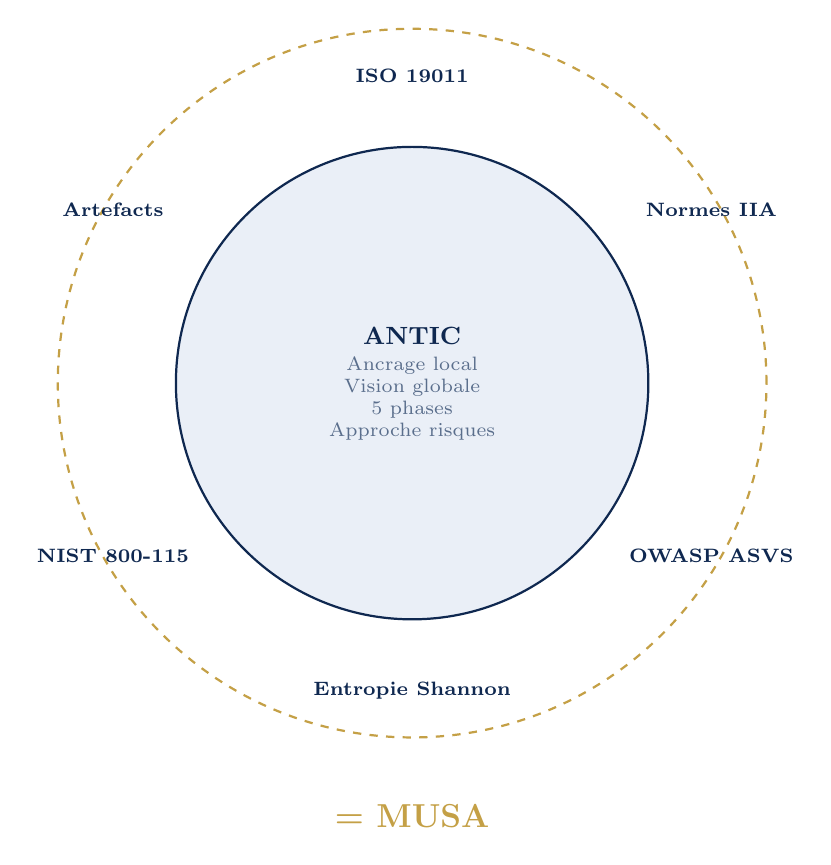
\begin{tikzpicture}[font=\small]
  % Cercle ANTIC
  \draw[navy, thick, fill=lightnavy!60] (0,0) circle (3cm);
  \node[align=center] at (0,0.6) {\textbf{\color{navy}ANTIC}};
  \node[align=center, font=\scriptsize\color{steel}] at (0,-0.2)
    {Ancrage local\\Vision globale\\5~phases\\Approche risques};
  % Cercle MUSA
  \draw[gold, dashed, thick] (0,0) circle (4.5cm);
  % Apports
  \node[align=center,font=\scriptsize\bfseries\color{navy}] at (0,3.9)
    {ISO~19011};
  \node[align=center,font=\scriptsize\bfseries\color{navy}] at (3.8,2.2)
    {Normes IIA};
  \node[align=center,font=\scriptsize\bfseries\color{navy}] at (3.8,-2.2)
    {OWASP~ASVS};
  \node[align=center,font=\scriptsize\bfseries\color{navy}] at (0,-3.9)
    {Entropie Shannon};
  \node[align=center,font=\scriptsize\bfseries\color{navy}] at (-3.8,-2.2)
    {NIST~800-115};
  \node[align=center,font=\scriptsize\bfseries\color{navy}] at (-3.8,2.2)
    {Artefacts};
  % Label MUSA
  \node[align=center,font=\large\bfseries\color{gold}] at (0,-5.5)
    {= MUSA};
\end{tikzpicture}
\caption{Positionnement de MUSA par rapport \`a la d\'emarche ANTIC}
\label{fig:musa}
\end{figure}

\section*{Conclusion du chapitre}
\addcontentsline{toc}{section}{Conclusion du chapitre}

Ce chapitre a pos\'e les fondements th\'eoriques et conduit une analyse syst\'ematique
de la d\'emarche ANTIC. Trois apports originaux \'emergent~: (1)~la justification de
la fusion audit s\'ecurit\'e~+ applicatif dans le contexte d'audit interne chez un
d\'eveloppeur~; (2)~l'introduction de l'entropie de Shannon comme mesure quantitative
in\'edite de la reproductibilit\'e inter-auditeurs~; (3)~l'identification de trois
nouvelles limites de l'ANTIC non document\'ees dans la litt\'erature~, absence
d'alignement ISO~19011, absence de gouvernance IIA, absence de mesure de la
reproductibilit\'e. Le chapitre~2 pr\'esentera la m\'ethode MUSA dans sa version
compl\`ete, en justifiant chaque choix par les \'ecarts identifi\'es.

% ── Références ────────────────────────────────────────────
\section*{R\'ef\'erences bibliographiques du chapitre~1}
\addcontentsline{toc}{section}{R\'ef\'erences bibliographiques du chapitre~1}

\begin{thebibliography}{99}

\bibitem{antic2020}
ANTIC. (2020). \textit{R\'ef\'erentiel interne d'audit de s\'ecurit\'e des
syst\`emes d'information}. Agence Nationale des Technologies de l'Information
et de la Communication, Yaound\'e.

\bibitem{antic_conf2026}
ANTIC. (2026). \textit{M\'ethodologie d'audit de s\'ecurit\'e des syst\`emes
d'information ; Pr\'esentation aux cabinets agr\'e\'es} [Source primaire non
publi\'ee]. Conf\'erence ANTIC, Yaound\'e, Cameroun, 29~avril~2026.

\bibitem{iso27000}
ISO/IEC~27000:2018. \textit{Technologies de l'information , Techniques de
s\'ecurit\'e , Vue d'ensemble et vocabulaire}. Organisation Internationale
de Normalisation.

\bibitem{iso27001}
ISO/IEC~27001:2022. \textit{S\'ecurit\'e de l'information ; Exigences}.
Organisation Internationale de Normalisation.

\bibitem{iso19011}
ISO~19011:2018. \textit{Lignes directrices pour l'audit des syst\`emes de
management}. Organisation Internationale de Normalisation.

\bibitem{iia_ippf}
Institute of Internal Auditors. (2017). \textit{International Professional
Practices Framework (IPPF)}. The IIA, Lake Mary, FL.

\bibitem{owasp_asvs}
OWASP Foundation. (2021). \textit{Application Security Verification Standard
v4.0.3}. Open Web Application Security Project.

\bibitem{nist800115}
Scarfone,~K., Souppaya,~M., Cody,~A., \& Orebaugh,~A. (2008). \textit{NIST
SP~800-115: Technical Guide to Information Security Testing and Assessment}.
National Institute of Standards and Technology.

\bibitem{nist80030}
NIST. (2012). \textit{SP~800-30 Rev.1: Guide for Conducting Risk Assessments}.
National Institute of Standards and Technology.

\bibitem{shannon1948}
Shannon,~C.~E. (1948). A Mathematical Theory of Communication. \textit{Bell
System Technical Journal}, \textit{27}(3), 379--423.

\bibitem{isaca2020}
ISACA. (2020). \textit{CISA Review Manual}. Information Systems Audit and
Control Association.

\bibitem{fenz2014}
Fenz,~S., Heurix,~J., Neubauer,~T., \& Pechstein,~F. (2014). Current Challenges
in Information Security Risk Management. \textit{Information Management \&
Computer Security}, \textit{22}(5), 410--430.

\bibitem{dhillon2000}
Dhillon,~G., \& Backhouse,~J. (2000). Information System Security Management
in the New Millennium. \textit{Communications of the ACM}, \textit{43}(7),
125--128.

\bibitem{stallings2018}
Stallings,~W. (2018). \textit{Cryptography and Network Security} (7\textsuperscript{th}~ed.). Pearson Education.

\bibitem{devsecops}
Kim,~G., Humble,~J., Debois,~P., \& Willis,~J. (2016). \textit{The DevOps
Handbook}. IT Revolution Press.

\bibitem{microsoft_sdl}
Microsoft. (2010). \textit{Security Development Lifecycle ; Process Guidance}.
Microsoft Corporation.

\bibitem{decret2002}
R\'epublique du Cameroun. (2002). \textit{D\'ecret
n\textdegree{}2002/092 du 27~mars~2002 portant cr\'eation de l'ANTIC}.
Pr\'esidence de la R\'epublique.

\bibitem{humphreys2016}
Humphreys,~E. (2016). \textit{Implementing the ISO/IEC~27001 ISMS Standard}.
Artech House.

\bibitem{bitlisli2024}
Bitlisli Erdivan,~P. (2024). \textit{An Information Security Assessment Model
for Very Small Entities}. Master thesis, Middle East Technical University.

\bibitem{chaiguide2014}
CHAI. (2014). \textit{Guide d'audit des syst\`emes d'information} (v1.0).
Secr\'etariat g\'en\'eral du CHAI, France.

\end{thebibliography}

% ============================================================
% ============================================================
%  CHAPITRE 2 -PROPOSITION DE MUSA
%  Méthode Unifiée d'Audit de Sécurité Applicative
% ============================================================

\decorativechapter{2}
  {Proposition de MUSA : M\'ethode Unifi\'ee\\[0.3em]
   d'Audit de S\'ecurit\'e Applicative}
  {Ce chapitre pr\'esente dans le d\'etail la m\'ethode MUSA~: ses principes
   directeurs, ses cinq phases op\'erationnelles, ses artefacts r\'eutilisables,
   ses m\'etriques et l'ensemble des outils qui la composent.}

\chapter{Proposition de MUSA : M\'ethode Unifi\'ee d'Audit de S\'ecurit\'e Applicative}
\minitoc

% ── Introduction ──────────────────────────────────────────
\section*{Introduction du chapitre}
\addcontentsline{toc}{section}{Introduction du chapitre}

Le chapitre pr\'ec\'edent a d\'emontr\'e, \`a travers une analyse syst\'ematique
de la d\'emarche ANTIC et une comparaison avec cinq standards internationaux,
qu'aucun r\'ef\'erentiel existant ne r\'epond simultan\'ement aux trois lacunes
fondamentales identifi\'ees~: le manque de reproductibilit\'e, la s\'eparation
artificielle entre s\'ecurit\'e et fonctionnement applicatif, et l'absence de
mesure objective de la qualit\'e de l'audit. Il a \'egalement montr\'e que
l'apport le plus original demand\'e~, l'\'evaluation simultan\'ee de la
s\'ecurit\'e et du fonctionnement~ est absent de l'ensemble des r\'ef\'erentiels
analys\'es.

Ce chapitre pr\'esente \textbf{MUSA} (\textit{M\'ethode Unifi\'ee d'Audit de
S\'ecurit\'e Applicative}), la m\'ethode qui r\'epond point par point \`a ces
lacunes. La pr\'esentation suit une progression logique~: des principes fondateurs
vers les d\'etails op\'erationnels, des structures g\'en\'erales vers les outils
concrets. Chaque choix m\'ethodologique est ancr\'e dans les \'ecarts identifi\'es
au chapitre~1.

Ce chapitre est structur\'e en sept sections~: (1)~les principes directeurs,
(2)~la structure globale de la m\'ethode, (3) \`a (6)~la description d\'etaill\'ee
des quatre phases, et (7)~la synth\`ese des apports.

% ============================================================
\section{Principes directeurs de MUSA}
\label{sec:principes}
% ============================================================

Avant toute description proc\'edurale, il est essentiel de poser les principes
qui gouvernent chaque d\'ecision m\'ethodologique de MUSA. Ces principes ne sont
pas des platitudes~: chacun r\'epond \`a une limite concr\`ete de la d\'emarche
ANTIC identifi\'ee au chapitre~1.

\subsection{Principe 1 - Reproductibilit\'e mesurable}

\textbf{Probl\`eme adress\'e~:} Limite L2 et L9 (tableau~1.17). Deux auditeurs
appliquant la m\^eme d\'emarche ANTIC peuvent obtenir des r\'esultats
fondamentalement diff\'erents.

\textbf{R\'eponse de MUSA~:} Toute appr\'eciation subjective est convertie en
donn\'ee num\'erique~: l'entropie de Shannon~$H_i$ mesure le niveau d'accord
entre auditeurs sur chaque assertion. Aucun constat ne peut \^etre valid\'e
directement si $H_i \geq 0{,}5$. La reproductibilit\'e n'est pas un objectif
d\'eclaratif~: c'est une valeur calcul\'ee, traçable, archiv\'ee dans les papiers
de travail.

\subsection{Principe 2 - Fusion d\'elib\'er\'ee s\'ecurit\'e + applicatif}

\textbf{Probl\`eme adress\'e~:} Crit\`ere C9 (tableau~1.18), absent de tous les
r\'ef\'erentiels existants. Dans le contexte d'audit interne chez un d\'eveloppeur,
la s\'ecurit\'e et le fonctionnement sont indissociables.

\textbf{R\'eponse de MUSA~:} Chaque phase de l'audit couvre simultan\'ement les
deux dimensions. Les checklists int\`egrent \`a la fois les contrôles de s\'ecurit\'e
(OWASP~ASVS) et les crit\`eres de conformit\'e fonctionnelle. Un m\^eme papier de
travail documente une vuln\'erabilit\'e de s\'ecurit\'e \textit{et} son impact sur
la logique m\'etier de l'application.

\paragraph{Précision sur la mise en œuvre de la fusion}

La fusion des audits de sécurité et fonctionnel dans MUSA repose sur 
une approche d'\textbf{équipe pluridisciplinaire}. L'équipe d'audit 
est composée d'au moins :

\begin{itemize}[label={\color{gold}\ding{70}}, leftmargin=*]
	\item \textbf{Un expert en sécurité applicative} : responsable des 
	tests techniques (SAST, DAST, configuration, tests d'intrusion).
	\item \textbf{Un expert métier} : responsable de la validation des 
	flux fonctionnels et de la logique comptable de GIDOCEP.
\end{itemize}

Ces deux profils travaillent en binôme sur les mêmes artefacts 
(checklists, papiers de travail), chacun apportant sa perspective 
spécifique. La \textit{fusion} ne signifie pas qu'une seule personne 
doit posséder les deux compétences, mais que les deux expertises 
sont \textbf{intégrées dans un même processus d'audit} et aboutissent 
à un \textbf{rapport unique}.

Cette approche est justifiée par le contexte SOLTEC : une PME ne 
peut financer deux missions d'audit séparées, mais peut en revanche 
mobiliser deux experts internes ou externes pour une mission unique.
\subsection{Principe 3 - Formalisation compl\`ete des proc\'edures}

\textbf{Probl\`eme adress\'e~:} Limite L1 (manque de formalisation). La qualit\'e
de l'audit ANTIC d\'epend de la comp\'etence personnelle de l'auditeur, non de la
m\'ethode.

\textbf{R\'eponse de MUSA~:} Chaque activit\'e de chaque phase est d\'ecrite avec
un niveau de d\'etail tel qu'un auditeur comp\'etent mais ne connaissant pas
MUSA puisse l'ex\'ecuter correctement \`a partir des seuls artefacts de la m\'ethode.
Aucune \'etape ne laisse de place \`a l'interpr\'etation discr\'etionnaire.

\subsection{Principe 4 - Profondeur adaptable \`a la criticit\'e}

\textbf{Probl\`eme adress\'e~:} Limite L5 (profondeur variable). L'ANTIC applique
le m\^eme niveau d'analyse ind\'ependamment de la criticit\'e de l'application.

\textbf{R\'eponse de MUSA~:} Trois niveaux d'audit sont d\'efinis, align\'es sur
l'OWASP~ASVS~: basique~(40~contr\^oles), standard~(100~contr\^oles), approfondi
(150~contr\^oles). Le niveau est d\'etermin\'e en phase~1 selon une grille de
criticit\'e objective. GIDOCEP est \'evalu\'e au niveau~2 (standard).

\subsection{Principe 5 - Gouvernance rigoureuse}

\textbf{Probl\`eme adress\'e~:} Limites L7 et L8 (absence ISO~19011 et gouvernance
IIA). L'ANTIC aspire \`a l'ISO~19011 sans l'avoir formalis\'e~; les normes IIA sont
absentes.

\textbf{R\'eponse de MUSA~:} Chaque phase de MUSA correspond \`a une phase de
l'ISO~19011. Chaque livrable formel (PV, d\'eclaration d'ind\'ependance, papiers
de travail) r\'epond \`a une norme IIA sp\'ecifique. La gouvernance n'est pas un
ajout~: elle est int\'egr\'ee dans la structure m\^eme de la m\'ethode.

\subsection{Principe 6 - R\'eutilisabilit\'e syst\'ematique}

\textbf{Probl\`eme adress\'e~:} Limite L8 (absence de m\'ethode r\'eutilisable).
Chaque mission ANTIC produit un rapport ponctuel qui ne capitalise pas.

\textbf{R\'eponse de MUSA~:} MUSA ne produit pas un rapport~: elle produit un
\textbf{capital m\'ethodologique}. Les checklists, papiers de travail, matrices de
risques et mod\`eles de rapport sont con\c{c}us pour \^etre r\'eutilis\'es \`a
chaque cycle d'audit et g\'en\'eralis\'es \`a d'autres applications. La qualit\'e
s'am\'eliore d'un cycle \`a l'autre car les artefacts sont enrichis.

\subsection{Principe 7 - Ancrage local pr\'eserv\'e}

\textbf{Probl\`eme adress\'e~:} Il serait contre-productif de remplacer la
d\'emarche ANTIC par un standard international inadapt\'e au contexte camerounais.

\textbf{R\'eponse de MUSA~:} MUSA \textit{enrichit} la d\'emarche ANTIC, elle ne la
remplace pas. La structure en cinq phases, l'ancrage r\'eglementaire (loi
n\textdegree{}2010/012), la vision globale (organisationnel + humain + physique +
technologique), l'approche par les risques~$P \times I$ et l'accompagnement
post-audit sont int\'egralement conserv\'es.

% ============================================================
\section{Structure globale de MUSA}
\label{sec:structure}
% ============================================================

\subsection{Vue d'ensemble architecturale}

MUSA s'organise en \textbf{cinq phases s\'equentielles}, chacune dot\'ee
d'activit\'es d\'etaill\'ees, de livrables normalis\'es, de m\'etriques calcul\'ees
et d'outils Excel d\'edi\'es. La figure~\ref{fig:musa_structure} illustre cette
organisation.

\begin{figure}[H]
\centering
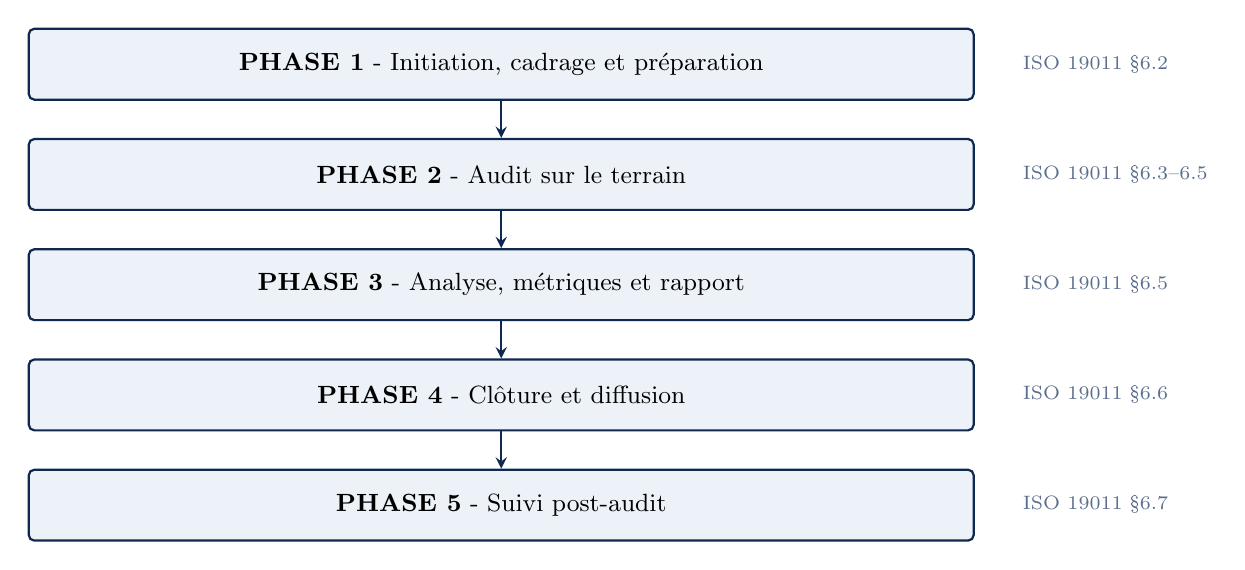
\begin{tikzpicture}[
  font=\small,
  phase/.style={
    rectangle, draw=navy, fill=lightnavy!50,
    minimum width=12cm, minimum height=0.9cm,
    align=center, rounded corners=2pt, thick
  },
  arrow/.style={->, >=stealth, thick, navy},
  label/.style={font=\scriptsize\color{steel}, align=left}
]
\node[phase] (p1) at (0,0)
  {\textbf{PHASE 1} - Initiation, cadrage et pr\'eparation};
\node[phase] (p2) at (0,-1.4)
  {\textbf{PHASE 2} - Audit sur le terrain};
\node[phase] (p3) at (0,-2.8)
  {\textbf{PHASE 3} - Analyse, m\'etriques et rapport};
\node[phase] (p4) at (0,-4.2)
  {\textbf{PHASE 4} - Cl\^oture et diffusion};
\node[phase] (p5) at (0,-5.6)
  {\textbf{PHASE 5} - Suivi post-audit};

\draw[arrow] (p1.south) -- (p2.north);
\draw[arrow] (p2.south) -- (p3.north);
\draw[arrow] (p3.south) -- (p4.north);
\draw[arrow] (p4.south) -- (p5.north);

% ISO 19011 reference
\node[label, anchor=west] at (6.5, 0)
  {ISO~19011 §6.2};
\node[label, anchor=west] at (6.5,-1.4)
  {ISO~19011 §6.3--6.5};
\node[label, anchor=west] at (6.5,-2.8)
  {ISO~19011 §6.5};
\node[label, anchor=west] at (6.5,-4.2)
  {ISO~19011 §6.6};
\node[label, anchor=west] at (6.5,-5.6)
  {ISO~19011 §6.7};
\end{tikzpicture}
\caption{Structure globale des cinq phases de MUSA}
\label{fig:musa_structure}
\end{figure}

\subsection{Les niveaux d'audit MUSA}

La profondeur de chaque audit est d\'etermin\'ee en Phase~1 selon le tableau
suivant~:

\begin{table}[H]
\centering\small
\caption{Les trois niveaux d'audit MUSA}
\label{tab:niveaux_musa}
\rowcolors{2}{trow1}{trow2}
\begin{tabularx}{\textwidth}{p{2.5cm}p{3cm}p{2cm}p{2cm}X}
\toprule
\rowcolor{theadcolor}
\color{white}\textbf{Niveau} &
\color{white}\textbf{Type d'application} &
\color{white}\textbf{Contr\^oles OWASP} &
\color{white}\textbf{Dur\'ee estim\'ee} &
\color{white}\textbf{Crit\`eres de d\'eclenchement} \\
\midrule
\textbf{1 - Basique} & Applications internes sans donn\'ees sensibles &
  40 & 3--5 jours & Aucune donn\'ee financi\`ere ni personnelle, faible impact \\
\textbf{2 - Standard} & Applications sensibles avec donn\'ees financi\`eres &
  100 & 7--10 jours & Donn\'ees personnelles ou financi\`eres, impact mod\'er\'e \\
\textbf{3 - Approfondi} & Applications critiques, forte exposition &
  150 & 15--20 jours & Donn\'ees tr\`es sensibles, obligations r\'eglementaires, acc\`es Internet \\
\bottomrule
\end{tabularx}
\end{table}

\textbf{Application \`a GIDOCEP~:} GIDOCEP g\`ere les op\'erations comptables
des \'etablissements publics camerounais~, donn\'ees financi\`eres sensibles,
utilisateurs identifi\'es, obligations r\'eglementaires ANTIC. Elle est class\'ee
\textbf{niveau~2 (Standard)}.

\subsection{Les artefacts MUSA}

MUSA produit sept cat\'egories d'artefacts op\'erationnels~:

\begin{table}[H]
\centering\small
\caption{Les sept cat\'egories d'artefacts MUSA}
\label{tab:artefacts}
\rowcolors{2}{trow1}{trow2}
\begin{tabularx}{\textwidth}{p{0.5cm}p{3.5cm}p{4cm}X}
\toprule
\rowcolor{theadcolor}
\color{white}\textbf{\#} &
\color{white}\textbf{Artefact} &
\color{white}\textbf{Format} &
\color{white}\textbf{Contenu et usage} \\
\midrule
A1 & Charte d'audit & Document Word/PDF &
  P\'erim\`etre, objectifs, niveau, composition \'equipe, sign\'ee par les deux parties \\
A2 & D\'eclaration d'ind\'ependance & Formulaire PDF &
  Conflicts d'int\'er\^ets d\'eclar\'es, sign\'ee par chaque auditeur (IIA~1100) \\
A3 & Programme de travail & Fichier Excel (PT00) &
  Planning d\'etaill\'e, t\^aches, responsables, jalons \\
A4 & Papiers de travail (PTxx) & Fichiers Excel cod\'es &
  Un fichier par phase~: PT01 (phase 1), PT02 (phase 2a), PT03 (phase 2b), PT04 (phase 2c), PT05 (phase 3) \\
A5 & Checklists techniques & Fichiers Excel d\'edi\'es &
  CL-ISO27001, CL-OWASP-N2, CL-NIST avec colonnes \'evaluation + preuve \\
A6 & Matrice des risques & Fichier Excel (MR) &
  Vuln\'erabilit\'es, cotation $P \times I$, priorisation, responsable, \'ech\'eance \\
A7 & Rapport d'audit & Document Word/PDF &
  7 sections normalis\'ees, m\'etriques calcul\'ees, sign\'e lead auditor \\
\bottomrule
\end{tabularx}
\end{table}

\subsection{Les m\'etriques MUSA}

MUSA calcule cinq indicateurs quantitatifs pour chaque mission~:

\begin{table}[H]
\centering\small
\caption{Les cinq m\'etriques calcul\'ees par MUSA}
\label{tab:metriques_musa}
\rowcolors{2}{trow1}{trow2}
\begin{tabularx}{\textwidth}{p{4cm}p{5cm}X}
\toprule
\rowcolor{theadcolor}
\color{white}\textbf{M\'etrique} &
\color{white}\textbf{Formule} &
\color{white}\textbf{Interpr\'etation} \\
\midrule
Taux de conformit\'e global &
  $TC = \dfrac{N_C}{N_{total}} \times 100$ &
  Pourcentage des contr\^oles jug\'es conformes \\
Taux par niveau OWASP &
  $TC_n = \dfrac{N_{C,n}}{N_{n}} \times 100$ &
  Conformit\'e pour le niveau $n$ (1, 2 ou 3) \\
Score de risque moyen &
  $\bar{R} = \dfrac{\sum R_i}{N_{vuln}}$ &
  Risque moyen, avec $R_i = P_i \times I_i$ \\
Entropie par assertion &
  $H_i = -\sum p_k \log_2 p_k$ &
  Niveau d'accord entre auditeurs \\
Entropie globale &
  $H_{global} = \dfrac{1}{N}\sum_{i=1}^N H_i$ &
  Reproductibilit\'e globale de la mission \\
\bottomrule
\end{tabularx}
\end{table}
\subsubsection{Exemple concret de calcul de l'entropie}

Pour illustrer le calcul de l'entropie de Shannon, prenons deux exemples issus de l'audit de GIDOCEP.

\paragraph{Exemple 1 : Accord fort}

\textbf{Assertion 1.1} : Politique de sécurité formelle et signée

\begin{table}[H]
	\centering\small
	\caption{Évaluations de l'assertion 1.1}
	\label{tab:entropie_exemple1}
	\begin{tabular}{|p{3.5cm}|c|c|c|c|}
		\hline
		\textbf{Assertion} & \textbf{Aud1} & \textbf{Aud2} & \textbf{Aud3} & \textbf{Hi} \\
		\hline
		Politique de sécurité formelle et signée & NC & NC & NC & 0,00 \\
		\hline
	\end{tabular}
\end{table}
\textbf{Calcul :}
\begin{itemize}[label={\color{gold}\ding{70}}, leftmargin=*]
	\item pC = 0/3 = 0,00
	\item pNC = 3/3 = 1,00
	\item pZG = 0/3 = 0,00
	\item $H = -(1{,}00 \times \log_{2}(1{,}00)) = 0{,}00$
\end{itemize}

\textbf{Interprétation} : Accord fort → constat validé directement.

\paragraph{Exemple 2 : Zone grise}

\textbf{Assertion 1.3} : RSSI identifié avec fiche de poste

\begin{table}[H]
	\centering\small
	\caption{Évaluations de l'assertion 1.3}
	\label{tab:entropie_exemple2}
	\begin{tabular}{|p{3.5cm}|c|c|c|c|}
		\hline
		\textbf{Assertion} & \textbf{Aud1} & \textbf{Aud2} & \textbf{Aud3} & \textbf{Hi} \\
		\hline
		RSSI identifié avec fiche de poste & C & NC & C & 0,91 \\
		\hline
	\end{tabular}
\end{table}
\textbf{Calcul :}
\begin{itemize}[label={\color{gold}\ding{70}}, leftmargin=*]
	\item pC = 2/3 = 0,67
	\item pNC = 1/3 = 0,33
	\item pZG = 0/3 = 0,00
	\item $H = -(0{,}67 \times \log_{2}(0{,}67) + 0{,}33 \times \log_{2}(0{,}33))$
	\item $H = -(0{,}67 \times (-0{,}58) + 0{,}33 \times (-1{,}58)) = 0{,}91$
\end{itemize}

\textbf{Interprétation} : $0{,}5 \leq H < 1{,}0$ → Discussion requise. 
\section{Phase 1 : Initiation, cadrage et pr\'eparation}
\label{sec:phase1}
% ============================================================

\subsection{Vue d'ensemble de la phase}

La Phase~1 est le fondement de toute la mission. Une pr\'eparation insuffisante
entra\^ine invariablement des lacunes dans les phases suivantes~: p\'erim\`etre
mal d\'elimit\'e, \'equipe inadapt\'ee, documents manquants. Cette phase est
align\'ee sur l'ISO~19011 §6.2 (d\'eclenchement) et §6.3 (pr\'eparation).

\begin{table}[H]
\centering\small
\caption{Vue synth\'etique de la Phase~1}
\label{tab:vue_p1}
\rowcolors{2}{trow1}{trow2}
\begin{tabularx}{\textwidth}{p{3.5cm}X}
\toprule
\rowcolor{theadcolor}
\color{white}\textbf{\'El\'ement} &
\color{white}\textbf{D\'etail} \\
\midrule
Dur\'ee typique & 5 \`a 7 jours ouvrables \\
Normes de r\'ef\'erence & ISO~19011 §6.2--6.3, IIA~2200, IIA~2210, IIA~2230 \\
Artefacts produits & Charte d'audit (A1), D\'eclaration d'ind\'ependance (A2), Programme de travail PT00 (A3) \\
Outil Excel d\'edi\'e & \textbf{PT01-Phase1.xlsx} \\
R\'eunion formelle & R\'eunion de lancement avec PV sign\'e \\
Crit\`ere de cl\^oture & Programme de travail approuv\'e par le commanditaire \\
\bottomrule
\end{tabularx}
\end{table}

\subsection{\'Etape 1.1 : D\'eclenchement et contact initial}

\subsubsection{Activit\'es}

Le d\'eclenchement de l'audit intervient sur demande formelle du commanditaire
(direction g\'en\'erale de SOLTEC ou point focal ANTIC). Les activit\'es
suivantes sont men\'ees~:

\begin{itemize}[label={\color{gold}\ding{70}}, leftmargin=*, itemsep=4pt]
\item \textbf{R\'eception et analyse du mandat~:} l'auditeur en charge prend
  connaissance de la demande, identifie l'application concern\'ee (GIDOCEP),
  les syst\`emes impliqu\'es et les parties prenantes.
\item \textbf{\'Evaluation de la faisabilit\'e~:} v\'erification que les ressources
  humaines, mat\'erielles et temporelles sont disponibles. Crit\`eres v\'erifi\'es~:
  comp\'etences n\'ecessaires disponibles dans l'\'equipe, fen\^etre temporelle
  compatible avec les contraintes de SOLTEC, acc\`es possible aux syst\`emes.
\item \textbf{Contact pr\'eliminaire avec l'audit\'e~:} le lead auditor prend contact
  avec le point focal de SOLTEC pour confirmer la disponibilit\'e et annoncer le
  d\'ebut de la mission.
\item \textbf{S\'election de l'\'equipe d'audit~:} constitution de l'\'equipe selon
  une grille de comp\'etences pond\'er\'ee (cf. tableau~\ref{tab:grille_equipe}).
\end{itemize}

\subsubsection{Grille de s\'election de l'\'equipe}

\begin{table}[H]
\centering\small
\caption{Grille de s\'election de l'\'equipe d'audit MUSA}
\label{tab:grille_equipe}
\rowcolors{2}{trow1}{trow2}
\begin{tabularx}{\textwidth}{p{4cm}p{2cm}p{1.5cm}X}
\toprule
\rowcolor{theadcolor}
\color{white}\textbf{Comp\'etence requise} &
\color{white}\textbf{Pond\'eration} &
\color{white}\textbf{Niveau min.} &
\color{white}\textbf{Justification} \\
\midrule
S\'ecurit\'e applicative & 30\,\% & Confirmé &
  Tests OWASP, injection, gestion session \\
Audit de SI (m\'ethodologie) & 25\,\% & Confirmé &
  Conduite d'audit selon ISO 19011 \\
D\'eveloppement logiciel & 20\,\% & Interm\'ediaire &
  Compr\'ehension de la logique GIDOCEP \\
Comptabilit\'e / m\'etier & 15\,\% & Notions &
  \'Evaluer la conformit\'e fonctionnelle \\
R\'eglementation TIC Cameroun & 10\,\% & Notions &
  Loi 2010/012, r\'ef\'erentiel ANTIC \\
\bottomrule
\end{tabularx}
\end{table}

\subsubsection{D\'eclaration d'ind\'ependance (Artefact A2)}

Avant toute activit\'e sur le terrain, chaque membre de l'\'equipe signe une
\textbf{d\'eclaration d'ind\'ependance} (IIA~1100). Ce document formalise~:

\begin{itemize}[label={\color{gold}\ding{70}}, leftmargin=*, itemsep=2pt]
\item l'absence de lien familial ou financier avec SOLTEC ou les d\'eveloppeurs de
  GIDOCEP~;
\item l'absence de participation ant\'erieure au d\'eveloppement ou \`a la
  maintenance de GIDOCEP~;
\item l'engagement \`a signaler tout conflit d'int\'er\^ets surgissant en cours
  de mission~;
\item la signature dat\'ee de l'auditeur et du lead auditor.
\end{itemize}

\subsubsection{Outil Excel - PT01-Phase1.xlsx}

La Phase~1 est document\'ee dans le fichier \textbf{PT01-Phase1.xlsx}, qui
comprend les onglets suivants~:

\begin{table}[H]
\centering\small
\caption{Structure du fichier PT01-Phase1.xlsx}
\label{tab:pt01}
\rowcolors{2}{trow1}{trow2}
\begin{tabularx}{\textwidth}{p{3cm}X}
\toprule
\rowcolor{theadcolor}
\color{white}\textbf{Onglet} &
\color{white}\textbf{Contenu} \\
\midrule
\texttt{Faisabilité} & Grille d'évaluation de la faisabilité (ressources, compétences, délais) \\
\texttt{Équipe} & Composition de l'équipe avec grille de compétences pondérée et scores \\
\texttt{Indépendance} & Formulaire de déclaration d'indépendance (une ligne par auditeur) \\
\texttt{Périmètre} & Délimitation du périmètre (inclus / exclus) avec justification \\
\texttt{Criticité} & Grille de détermination du niveau d'audit (1, 2 ou 3) \\
\texttt{Planning} & Programme de travail détaillé par phase, tâche, responsable, durée \\
\texttt{Documents demandés} & Liste des documents à collecter avec critères d'acceptabilité \\
\texttt{PV Lancement} & Modèle de procès-verbal de la réunion de lancement \\
\bottomrule
\end{tabularx}
\end{table}

\subsection{\'Etape 1.2 : D\'efinition du p\'erim\`etre et du niveau d'audit}

\subsubsection{D\'elimitaiton du p\'erim\`etre}

Le p\'erim\`etre de l'audit doit \^etre d\'efini avec pr\'ecision avant toute
activit\'e sur le terrain. Pour GIDOCEP, le p\'erim\`etre inclut~:

\begin{itemize}[label={\color{gold}\ding{70}}, leftmargin=*, itemsep=2pt]
\item \textbf{Inclus~:} l'application GIDOCEP dans sa version d\'eploy\'ee en
  production, le serveur h\'ebergeant l'application, la base de donn\'ees
  associ\'ee, les interfaces utilisateurs, les API internes.
\item \textbf{Exclus~:} l'infrastructure r\'eseau de l'\'etablissement client,
  les postes de travail des utilisateurs finaux (sauf \'echantillon),
  les applications tierces non d\'evelopp\'ees par SOLTEC.
\end{itemize}

\subsubsection{Grille de d\'etermination du niveau}

\begin{table}[H]
\centering\small
\caption{Grille de d\'etermination du niveau d'audit pour GIDOCEP}
\label{tab:niveau_gidocep}
\rowcolors{2}{trow1}{trow2}
\begin{tabularx}{\textwidth}{p{5cm}p{2cm}p{2cm}X}
\toprule
\rowcolor{theadcolor}
\color{white}\textbf{Crit\`ere} &
\color{white}\textbf{R\'eponse} &
\color{white}\textbf{Score} &
\color{white}\textbf{Justification} \\
\midrule
Donn\'ees financi\`eres trait\'ees & Oui & +2 & Ecritures comptables publiques \\
Donn\'ees personnelles & Oui & +1 & Identit\'es des agents comptables \\
Acc\`es Internet direct & Non & 0 & Application intranet \\
Obligations r\'eglementaires & Oui & +1 & Audit ANTIC obligatoire \\
Impact si compromission & \'Elev\'e & +2 & Finances publiques camerounaises \\
Migrations pr\'evues & Oui & +1 & Transition cloud envisag\'ee \\
\midrule
\textbf{Score total} & & \textbf{7} & \textbf{Niveau~2 (Standard) , seuil : 5--8} \\
\bottomrule
\end{tabularx}
\end{table}

\subsection{\'Etape 1.3 : Collecte documentaire pr\'ealable}

La collecte documentaire pr\'ealable (phase passive) permet de construire une
compr\'ehension du contexte avant d'aller sur le terrain. Elle suit des
\textbf{crit\`eres d'acceptabilit\'e} document\'es dans l'onglet
\texttt{Documents demandés} du fichier PT01.

\subsubsection{Crit\`eres d'acceptabilit\'e des documents}

Tout document collect\'e est \'evalu\'e selon trois crit\`eres~:

\begin{itemize}[label={\color{gold}\ding{70}}, leftmargin=*, itemsep=2pt]
\item \textbf{Fra\^icheur~:} le document doit dater de moins de 12~mois pour
  les politiques et moins de 6~mois pour les configurations.
\item \textbf{Authenticit\'e~:} le document doit \^etre sign\'e ou valid\'e
  par un responsable identifi\'e chez SOLTEC.
\item \textbf{Compl\'etude~:} un document incomplet est signal\'e comme
  \textit{partiellement acceptable} et d\'eclenche une demande compl\'ementaire.
\end{itemize}

\subsubsection{Liste des documents demand\'es}

\begin{table}[H]
\centering\small
\caption{Documents demand\'es en Phase~1 avec crit\`eres d'acceptabilit\'e}
\label{tab:docs_p1}
\rowcolors{2}{trow1}{trow2}
\begin{tabularx}{\textwidth}{p{4.5cm}p{2cm}p{2cm}X}
\toprule
\rowcolor{theadcolor}
\color{white}\textbf{Document} &
\color{white}\textbf{Cat\'egorie} &
\color{white}\textbf{Fra\^icheur max.} &
\color{white}\textbf{Crit\`ere de validation} \\
\midrule
Politique de s\'ecurit\'e & Organisationnel & 12 mois & Sign\'ee DG \\
Charte informatique & Organisationnel & 24 mois & Sign\'ee RH + DSI \\
Sch\'ema d'architecture GIDOCEP & Technique & 6 mois & Valid\'e lead dev \\
Inventaire des composants tiers & Technique & 6 mois & Liste avec versions \\
Proc\'edures de gestion des incidents & Op\'erationnel & 12 mois & Num\'erot\'ee, dat\'ee \\
Rapports d'audits ant\'erieurs & Historique & 3 ans & Officiel ANTIC ou tiers \\
Manuel d'installation / d\'eploiement & Technique & 12 mois & Version coh\'erente avec prod. \\
Proc\'edure de gestion des acc\`es & Organisationnel & 12 mois & Sign\'ee responsable SI \\
Plan de reprise d'activit\'e (PRA) & Op\'erationnel & 12 mois & Test\'e, dat\'e \\
Journal des modifications r\'ecentes & Technique & 3 mois & Syst\`eme de versioning \\
\bottomrule
\end{tabularx}
\end{table}

\subsection{\'Etape 1.4 : R\'eunion de lancement}

La r\'eunion de lancement est une exigence formelle de l'ISO~19011~§6.4.2. Elle
ne peut pas \^etre remplac\'ee par un \'echange de courriels.

\subsubsection{Participants obligatoires}

\begin{itemize}[label={\color{gold}\ding{70}}, leftmargin=*, itemsep=2pt]
\item Le lead auditor et l'\'equipe d'audit compl\`ete~;
\item Le directeur g\'en\'eral de SOLTEC ou son repr\'esentant mandaté~;
\item Le responsable technique de GIDOCEP~;
\item Le point focal ANTIC (si audit externe).
\end{itemize}

\subsubsection{Ordre du jour obligatoire}

\begin{enumerate}[leftmargin=*, itemsep=2pt]
\item Pr\'esentation de l'\'equipe d'audit et de ses mandats~;
\item Confirmation du p\'erim\`etre et du niveau d'audit~;
\item Pr\'esentation du calendrier et des jalons~;
\item D\'efinition des canaux de communication et des points de contact~;
\item R\`egles de confidentialit\'e et de diffusion des r\'esultats~;
\item Pr\'esentation des documents demand\'es et des d\'elais de fourniture~;
\item Questions et clarifications~;
\item Signature du PV de lancement par toutes les parties.
\end{enumerate}

\subsubsection{Livrables de la Phase~1}

\begin{goldbox}[title={\color{navy}\bfseries Livrables obligatoires de la Phase~1}]
\begin{enumerate}[leftmargin=*, itemsep=3pt]
\item \textbf{Charte d'audit sign\'ee} (A1)~: p\'erim\`etre, niveau, calendrier, composition \'equipe
\item \textbf{D\'eclarations d'ind\'ependance sign\'ees} (A2)~: une par auditeur
\item \textbf{Programme de travail approuv\'e} (PT00)~: planning d\'etaill\'e par t\^ache
\item \textbf{PV de r\'eunion de lancement sign\'e} (onglet \texttt{PV Lancement} du PT01)
\item \textbf{Dossier documentaire collect\'e} (avec grille de validation des documents)
\end{enumerate}
\end{goldbox}

% ============================================================
\section{Phase 2 : Audit sur le terrain}
\label{sec:phase2}
% ============================================================

\subsection{Vue d'ensemble}

La Phase~2 est la phase centrale de l'audit. Elle se d\'ecompose en
\textbf{trois sous-phases} men\'ees de mani\`ere coordonn\'ee, chacune
dot\'ee de son propre outil Excel~:

\begin{itemize}[label={\color{gold}\ding{70}}, leftmargin=*, itemsep=4pt]
\item \textbf{Sous-phase 2a} : Audit organisationnel et physique
\item \textbf{Sous-phase 2b} : Audit technique (SAST, DAST, configuration)
\item \textbf{Sous-phase 2c} : Analyse des risques et \'evaluation de la maturit\'e
\end{itemize}

\begin{table}[H]
\centering\small
\caption{Vue synth\'etique de la Phase~2}
\label{tab:vue_p2}
\rowcolors{2}{trow1}{trow2}
\begin{tabularx}{\textwidth}{p{3.5cm}X}
\toprule
\rowcolor{theadcolor}
\color{white}\textbf{\'El\'ement} &
\color{white}\textbf{D\'etail} \\
\midrule
Dur\'ee typique & 7 \`a 10 jours ouvrables (niveau~2) \\
Normes de r\'ef\'erence & ISO~19011 §6.4--6.5, IIA~2300--2340, OWASP~ASVS N2, NIST~SP~800-115 \\
Outils Excel d\'edi\'es & PT02-Audit-Orga.xlsx, PT03-Audit-Technique.xlsx, PT04-Risques.xlsx \\
R\'eunion formelle d'ouverture & PV sign\'e avant toute activit\'e sur le terrain \\
R\`egle de preuve & Aucune d\'eclaration n'est accept\'ee sans preuve documentaire \\
\bottomrule
\end{tabularx}
\end{table}

\subsection{R\'eunion d'ouverture}

Avant de d\'ebuter les activit\'es sur le terrain, une \textbf{r\'eunion
d'ouverture formelle} est tenue (ISO~19011~§6.4.2). Elle diff\`ere de la
r\'eunion de lancement~: celle-ci a eu lieu avant le terrain, pour poser les
bases~; la r\'eunion d'ouverture marque le d\'ebut concret des investigations.

\textbf{Dur\'ee~:} 30 \`a 45 minutes. \textbf{PV sign\'e~:} obligatoire.

\textbf{Points couverts~:}
\begin{enumerate}[leftmargin=*, itemsep=2pt]
\item Confirmation que le p\'erim\`etre et les objectifs n'ont pas chang\'e~;
\item Pr\'esentation du calendrier d\'etaill\'e des activit\'es du terrain~;
\item Confirmation des interlocuteurs disponibles et de leur plage horaire~;
\item Rappel des r\`egles de confidentialit\'e~;
\item Rappel que les d\'eclarations verbales ne constituent pas des preuves~;
\item Questions des parties.
\end{enumerate}

\subsection{Sous-phase 2a : Audit organisationnel et physique}

\subsubsection{Objectifs}

Cette sous-phase \'evalue les dimensions organisationnelle, humaine et physique
de la s\'ecurit\'e de GIDOCEP, conform\'ement \`a la vision globale de l'ANTIC
(quatre axes) et aux contr\^oles ISO~27001 domaines~5,~6 et~7.

\subsubsection{Entretiens standardis\'es}

Les entretiens sont men\'es avec trois cat\'egories d'interlocuteurs. Des
guides d'entretien distincts sont utilis\'es pour chaque cat\'egorie (annexes~F,~G,~H).

\begin{table}[H]
\centering\small
\caption{Guides d'entretien par profil d'interlocuteur}
\label{tab:guides_entretien}
\rowcolors{2}{trow1}{trow2}
\begin{tabularx}{\textwidth}{p{3cm}p{3cm}p{3cm}X}
\toprule
\rowcolor{theadcolor}
\color{white}\textbf{Profil} &
\color{white}\textbf{Th\`emes principaux} &
\color{white}\textbf{Dur\'ee} &
\color{white}\textbf{Preuves demand\'ees} \\
\midrule
Direction / DG & Politique de s\'ecurit\'e, budget, gouvernance &
  45--60 min & Politique sign\'ee, budget allou\'e \\
Responsable technique / Devs & Pratiques de codage, gestion des acc\`es, tests &
  60--90 min & Code, procédures, historique des tests \\
Utilisateurs finaux & Pratiques d'authentification, comportements &
  20--30 min & \'Echantillon de 3--5 utilisateurs \\
\bottomrule
\end{tabularx}
\end{table}

\subsubsection{R\`egle fondamentale de collecte de preuves}

\begin{goldbox}
\textbf{R\`egle MUSA~:} Toute affirmation d'un interlocuteur doit \^etre
corrobor\'ee par une preuve documentaire, technique ou observationnelle.
\textit{Exemple~: un responsable d\'eclare que les mots de passe sont chiffr\'es.
L'auditeur ne valide pas sur cette seule d\'eclaration~; il demande un extrait
de code ou examine directement la base de donn\'ees.}
\end{goldbox}

\subsubsection{Grille d'inspection physique}

L'inspection physique est men\'ee avec la grille structur\'ee de l'annexe~E.
Les zones inspecties pour GIDOCEP sont~:

\begin{itemize}[label={\color{gold}\ding{70}}, leftmargin=*, itemsep=2pt]
\item Salle serveur / local technique~: climatisation, onduleurs, contr\^ole
  d'acc\`es, extinction incendie~;
\item Postes de travail des utilisateurs~: \'ecran verrouill\'e, mots de passe
  visibles, antivirus actif~;
\item Imprimantes~: documents sensibles non r\'ecup\'er\'es, acc\`es contr\^ol\'e~;
\item Zones de passage~: badges visibles, acc\`es non autoris\'e possible.
\end{itemize}

\subsubsection{Outil Excel - PT02-Audit-Orga.xlsx}

\begin{table}[H]
\centering\small
\caption{Structure du fichier PT02-Audit-Orga.xlsx}
\label{tab:pt02}
\rowcolors{2}{trow1}{trow2}
\begin{tabularx}{\textwidth}{p{4cm}X}
\toprule
\rowcolor{theadcolor}
\color{white}\textbf{Onglet} &
\color{white}\textbf{Contenu} \\
\midrule
\texttt{Entretien-Direction} & Guide d'entretien direction avec cases de saisie + preuve attendue + score \\
\texttt{Entretien-Devs} & Guide d'entretien développeurs avec cases + preuve + score \\
\texttt{Entretien-Utilisateurs} & Guide d'entretien utilisateurs avec cases + observation \\
\texttt{Inspection-Physique} & Grille d'inspection physique (cases C/NC/NA + observations) \\
\texttt{ISO27001-Orga} & Contrôles ISO 27001 domaines 5, 6, 7 avec évaluation + preuve \\
\texttt{Entropie-Orga} & Calcul automatique de $H_i$ pour chaque assertion évaluée collectivement \\
\texttt{Synthèse-2a} & Tableau de synthèse : forces, NC, zone grise, métriques \\
\bottomrule
\end{tabularx}
\end{table}

\subsection{Sous-phase 2b : Audit technique}

\subsubsection{Objectifs et cadre m\'ethodologique}

La sous-phase~2b applique la m\'ethodologie NIST~SP~800-115 (planification,
ex\'ecution, post-exploitation) et l'OWASP~ASVS niveau~2 (\textbf{100 contr\^oles
sur 14 cat\'egories}) \`a GIDOCEP.

\textbf{Condition pr\'ealable obligatoire~:} une \textbf{autorisation \'ecrite
de test sign\'ee} par le directeur g\'en\'eral de SOLTEC est exig\'ee avant tout
test intrusif. Ce document pr\'ecise~: le p\'erim\`etre technique autoris\'e,
la p\'eriode d'ex\'ecution, les techniques autoris\'ees et celles interdites,
les contacts d'urgence en cas d'incident.

\subsubsection{S\'election et utilisation des outils}

Conform\'ement au NIST~SP~800-115, MUSA exige l'utilisation d'\textbf{au moins
deux outils distincts} pour chaque type de scan, afin de limiter les faux positifs
et faux n\'egatifs.

\begin{table}[H]
\centering\small
\caption{Outils recommand\'es pour l'audit technique de GIDOCEP}
\label{tab:outils_tech}
\rowcolors{2}{trow1}{trow2}
\begin{tabularx}{\textwidth}{p{3cm}p{2.5cm}p{2.5cm}X}
\toprule
\rowcolor{theadcolor}
\color{white}\textbf{Type de test} &
\color{white}\textbf{Outil principal} &
\color{white}\textbf{Outil secondaire} &
\color{white}\textbf{Cat\'egories OWASP cibl\'ees} \\
\midrule
SAST (statique) & SonarQube & Semgrep & V5, V10, V14 \\
DAST (dynamique) & OWASP~ZAP & Burp~Suite~Community & V2, V3, V5, V7 \\
Scan r\'eseau & Nmap & Masscan & V9, V14 \\
Scan vuln\'erabilit\'es & OpenVAS & Nikto & V8, V9, V14 \\
Chiffrement & SSLScan & testssl.sh & V6, V9 \\
Injection SQL & SQLMap & Test manuel & V5.3 \\
Contr\^ole d'acc\`es & Test manuel & Burp~Repeater & V4 \\
Authentification & Hydra (test limit\'e) & Test manuel & V2 \\
\bottomrule
\end{tabularx}
\end{table}

\subsubsection{D\'eroulement des tests techniques}

Les tests sont ex\'ecut\'es dans l'ordre suivant, con\c{c}u pour minimiser les
risques de perturbation de GIDOCEP~:

\begin{enumerate}[leftmargin=*, itemsep=4pt]
\item \textbf{Analyse statique du code source (SAST)~:} SonarQube analyse
  l'ensemble de la base de code GIDOCEP. Les r\'esultats sont export\'es en
  CSV et int\'egr\'es dans l'outil PT03. Cette \'etape ne pertube pas
  l'application en production.

\item \textbf{Revue de configuration~:} v\'erification manuelle des fichiers
  de configuration (serveur web, base de donn\'ees, pare-feu). Points v\'erifi\'es~:
  comptes par d\'efaut, mots de passe en clair, ports ouverts, modules
  inutiles activ\'es.

\item \textbf{Scan de vuln\'erabilit\'es r\'eseau~:} Nmap cartographie les
  services actifs~; OpenVAS effectue un scan de vuln\'erabilit\'es. Ex\'ecutable
  sur l'environnement de recette avant d'\'eventuellement passer en production.

\item \textbf{Test dynamique (DAST)~:} OWASP~ZAP teste l'application en
  ex\'ecution. Les tests suivants sont conduits~: injection SQL, XSS r\'efl\'echi
  et persistant, CSRF, gestion de session, contr\^ole d'acc\`es (IDOR).

\item \textbf{Tests d'authentification~:} v\'erification de la robustesse
  de l'authentification~: politique de mots de passe, blocage apr\`es \'echecs,
  s\'ecurit\'e des sessions, proc\'edure de r\'einitialisation.

\item \textbf{Tests de contr\^ole d'acc\`es~:} tentatives d'acc\`es non
  autoris\'es entre profils (utilisateur simple accédant aux fonctions admin,
  acc\`es aux donn\'ees d'un autre \'etablissement).

\item \textbf{Tests de logique m\'etier (sp\'ecifique GIDOCEP)~:} tentatives de
  contournement des flux comptables~: saisie d'\'ecritures hors-p\'eriode,
  modification r\'etroactive, contournement du workflow de validation.
\end{enumerate}

\subsubsection{Documentation des preuves}

Pour chaque vuln\'erabilit\'e identifi\'ee, l'auditeur documente obligatoirement~:

\begin{itemize}[label={\color{gold}\ding{70}}, leftmargin=*, itemsep=2pt]
\item une capture d'\'ecran ou un extrait de log d\'emontrant la vuln\'erabilit\'e~;
\item la proc\'edure de reproduction (\'etapes exactes)~;
\item la cat\'egorie OWASP~ASVS correspondante~;
\item le r\'ef\'erentiel ISO~27001 concern\'e~;
\item la cotation de gravit\'e (selon \'echelle CVSS ou $P \times I$).
\end{itemize}

\subsubsection{Outil Excel - PT03-Audit-Technique.xlsx}

\begin{table}[H]
\centering\small
\caption{Structure du fichier PT03-Audit-Technique.xlsx}
\label{tab:pt03}
\rowcolors{2}{trow1}{trow2}
\begin{tabularx}{\textwidth}{p{4cm}X}
\toprule
\rowcolor{theadcolor}
\color{white}\textbf{Onglet} &
\color{white}\textbf{Contenu} \\
\midrule
\texttt{OWASP-V1-V7} & Contrôles OWASP ASVS V1 à V7 (niveau 2) avec colonnes C/NC/ZG + preuve + $H_i$ \\
\texttt{OWASP-V8-V14} & Contrôles OWASP ASVS V8 à V14 (niveau 2) avec colonnes C/NC/ZG + preuve + $H_i$ \\
\texttt{NIST-Exécution} & Grille NIST SP 800-115 phase exécution (techniques, outils, résultats) \\
\texttt{Résultats-SAST} & Import CSV SonarQube + classification par sévérité + mapping OWASP \\
\texttt{Résultats-DAST} & Résultats OWASP ZAP + Burp Suite + classement \\
\texttt{Config-Serveur} & Checklist configuration serveur web, BDD, OS \\
\texttt{Logique-Métier} & Points de contrôle spécifiques à GIDOCEP (flux comptables, validation) \\
\texttt{ISO27001-Tech} & Contrôles ISO 27001 domaine 8 (mesures technologiques) \\
\texttt{Entropie-Tech} & Calcul automatique de $H_i$ pour assertions évaluées collectivement \\
\texttt{Synthèse-2b} & Tableau de synthèse : NC par catégorie OWASP, métriques \\
\bottomrule
\end{tabularx}
\end{table}
\subsection{Sous-phase 2c: Analyse des risques et \'evaluation de la maturit\'e}

\subsubsection{Matrice des risques}

L'ANTIC utilise une matrice $P \times I$ que MUSA conserve et formalise
enti\`erement. $P$ (probabilit\'e) et $I$ (impact) sont deux \'echelles
\textbf{compl\`etement ind\'ependantes}, chacune cot\'ee de~1 \`a~4.
Le score de risque $R = P \times I$ est \textbf{calcul\'e} par l'auditeur
pour chaque vuln\'erabilit\'e~; il n'est jamais pr\'ed\'efini. $R$
peut donc prendre toute valeur enti\`ere entre~1 et~16 selon les
combinaisons de $P$ et de $I$ retenues, soit \textbf{16 combinaisons
	possibles}.

\begin{figure}[H]
	\centering
	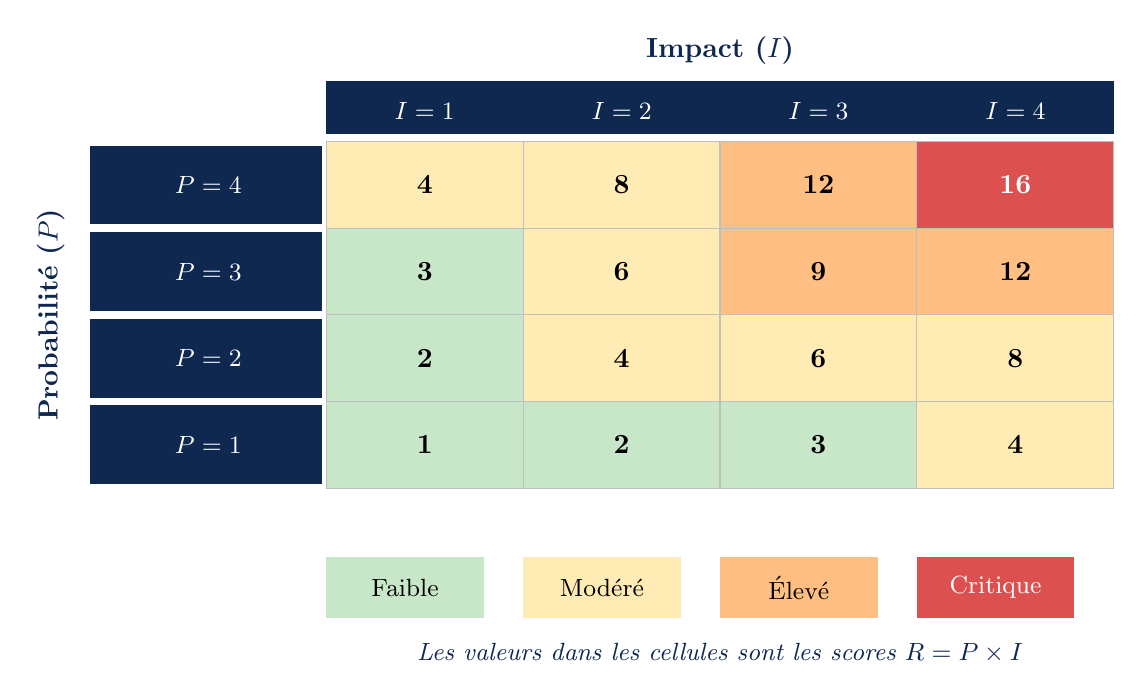
\begin{tikzpicture}[font=\small]
		% Couleurs par niveau de risque
		\definecolor{cFaible}{RGB}{200,230,200}
		\definecolor{cModere}{RGB}{255,235,180}
		\definecolor{cEleve}{RGB}{255,190,130}
		\definecolor{cCritique}{RGB}{220,80,80}
		
		% Taille des cellules
		\def\cw{2.5}
		\def\ch{1.1}
		
		% Matrice 4x4 — colonnes = I (1..4), lignes = P (4..1 de haut en bas)
		\foreach \row/\pval in {1/4, 2/3, 3/2, 4/1}{
			\foreach \col/\ival in {1/1, 2/2, 3/3, 4/4}{
				\pgfmathsetmacro{\rval}{int(\pval*\ival)}
				% Couleur selon le score
				\pgfmathsetmacro{\isC}{ifthenelse(\rval==16,1,0)}
				\pgfmathsetmacro{\isE}{ifthenelse(\rval>=9,1,0)}
				\pgfmathsetmacro{\isM}{ifthenelse(\rval>=4,1,0)}
				\ifnum\rval=16
				\def\cellcolor{cCritique}
				\def\textcol{white}
				\else\ifnum\rval>8
				\def\cellcolor{cEleve}
				\def\textcol{black}
				\else\ifnum\rval>3
				\def\cellcolor{cModere}
				\def\textcol{black}
				\else
				\def\cellcolor{cFaible}
				\def\textcol{black}
				\fi\fi\fi
				\fill[\cellcolor]
				({(\col-1)*\cw}, {-(\row-1)*\ch}) rectangle
				({(\col)*\cw},   {-(\row)*\ch});
				\draw[gray!50, line width=0.4pt]
				({(\col-1)*\cw}, {-(\row-1)*\ch}) rectangle
				({(\col)*\cw},   {-(\row)*\ch});
				\node[\textcol, font=\bfseries\normalsize] at
				({(\col-0.5)*\cw}, {-(\row-0.5)*\ch})
				{\rval};
			}
		}
		
		% En-têtes colonnes (Impact I)
		\foreach \col/\ival in {1/1, 2/2, 3/3, 4/4}{
			\fill[navy] ({(\col-1)*\cw}, 0.1) rectangle ({(\col)*\cw}, \ch*0.7);
			\node[white, font=\bfseries\small] at ({(\col-0.5)*\cw}, \ch*0.35)
			{$I = \ival$};
		}
		\node[navy, font=\bfseries] at ({2*\cw}, {\ch*1.05})
		{Impact ($I$)};
		
		% En-têtes lignes (Probabilité P)
		\foreach \row/\pval in {1/4, 2/3, 3/2, 4/1}{
			\fill[navy] ({-\cw*1.2}, {-(\row-1)*\ch-0.05}) rectangle
			({-0.05},    {-(\row)*\ch+0.05});
			\node[white, font=\bfseries\small] at ({-\cw*0.6}, {-(\row-0.5)*\ch})
			{$P = \pval$};
		}
		\node[navy, font=\bfseries, rotate=90] at ({-\cw*1.4}, {-2*\ch})
		{Probabilit\'e ($P$)};
		
		% Légende
		\def\ly{-4.8*\ch}
		\fill[cFaible]   (0,\ly) rectangle (\cw*0.8, \ly-\ch*0.7);
		\node[black, font=\small] at ({\cw*0.4}, {\ly-\ch*0.35}) {Faible};
		\fill[cModere]   (\cw*1.0,\ly) rectangle (\cw*1.8, \ly-\ch*0.7);
		\node[black, font=\small] at ({\cw*1.4}, {\ly-\ch*0.35}) {Mod\'er\'e};
		\fill[cEleve]    (\cw*2.0,\ly) rectangle (\cw*2.8, \ly-\ch*0.7);
		\node[black, font=\small] at ({\cw*2.4}, {\ly-\ch*0.35}) {\'Elev\'e};
		\fill[cCritique] (\cw*3.0,\ly) rectangle (\cw*3.8, \ly-\ch*0.7);
		\node[white, font=\small] at ({\cw*3.4}, {\ly-\ch*0.35}) {Critique};
		
		\node[font=\small\itshape, navy] at ({2*\cw}, {\ly-\ch*1.1})
		{Les valeurs dans les cellules sont les scores $R = P \times I$};
	\end{tikzpicture}
	\caption{Matrice visuelle des risques $R = P \times I$ --- MUSA}
	\label{fig:matrice_risque}
\end{figure}

\begin{table}[H]
	\centering\small
	\caption{\'Echelle de la probabilit\'e $P$ dans MUSA}
	\label{tab:echelle_P}
	% ── Échelle de Probabilité ────────────────────────────────
	\begin{tabularx}{\textwidth}{p{1.5cm}p{4cm}X}
		\toprule
		\rowcolor{theadcolor}
		\color{white}\textbf{Valeur $P$} &
		\color{white}\textbf{Niveau} &
		\color{white}\textbf{Crit\`eres d\'eterminants} \\
		\midrule
		$P = 1$ & Tr\`es faible &
		Exploitation tr\`es difficile~; conditions exceptionnelles~; aucun outil
		public disponible~; acc\`es physique ou privil\`ege \'elev\'e requis \\
		$P = 2$ & Faible &
		Exploitation possible par un attaquant exp\'eriment\'e~; outils sp\'ecialis\'es
		n\'ecessaires~; conditions particuli\`eres requises \\
		$P = 3$ & Mod\'er\'e &
		Exploitation accessible avec des outils courants~; techniques document\'ees
		publiquement~; aucune condition particuli\`ere n\'ecessaire \\
		$P = 4$ & \'Elev\'e &
		Exploitation triviale~; preuve de concept (PoC) publiquement disponible~;
		aucune comp\'etence sp\'eciale requise \\
		\bottomrule
	\end{tabularx}
\end{table}

\begin{table}[H]
	\centering\small
	\caption{\'Echelle de l'impact $I$ dans MUSA}
	\label{tab:echelle_I}
	\rowcolors{2}{trow1}{trow2}
	\begin{tabularx}{\textwidth}{p{1.5cm}p{4cm}X}
		\toprule
		\rowcolor{theadcolor}
		\color{white}\textbf{Valeur $I$} &
		\color{white}\textbf{Niveau} &
		\color{white}\textbf{Crit\`eres d\'eterminants} \\
		\midrule
		$I = 1$ & N\'egligeable &
		Aucune donn\'ee sensible affect\'ee~; aucune interruption de service~;
		impact financier nul ou marginal \\
		$I = 2$ & Limit\'e &
		Fuite de donn\'ees non sensibles ou d\'egradation partielle du service~;
		impact financier limit\'e~; correction sans urgence \\
		$I = 3$ & Significatif &
		Compromission partielle des donn\'ees comptables~; interruption de service
		notable~; risque de responsabilit\'e l\'egale~; impact financier mod\'er\'e \\
		$I = 4$ & Critique &
		Compromission totale de GIDOCEP~; acc\`es non autoris\'e \`a l'ensemble
		des donn\'ees financi\`eres publiques~; risque p\'enal~; impact financier
		majeur pour les \'etablissements publics concern\'es \\
		\bottomrule
	\end{tabularx}
\end{table}

\begin{table}[H]
	\centering\small
	\caption{Classification du risque $R = P \times I$ et seuils de priorit\'e}
	\label{tab:risque_classification}
	\rowcolors{2}{trow1}{trow2}
	\begin{tabularx}{\textwidth}{p{2.5cm}p{3cm}p{4.5cm}X}
		\toprule
		\rowcolor{theadcolor}
		\color{white}\textbf{Plage de $R$} &
		\color{white}\textbf{Niveau de risque} &
		\color{white}\textbf{Exemples $P \times I$} &
		\color{white}\textbf{D\'elai de correction impos\'e} \\
		\midrule
		$R \in [1,\,3]$ & \textbf{Faible} &
		$1{\times}1{=}1$~|~$1{\times}2{=}2$~|~$1{\times}3{=}3$~|~$3{\times}1{=}3$ &
		Planifi\'e (prochain cycle) \\
		$R \in [4,\,8]$ & \textbf{Mod\'er\'e} &
		$2{\times}2{=}4$~|~$2{\times}3{=}6$~|~$2{\times}4{=}8$~|~$4{\times}2{=}8$ &
		Correction dans le mois \\
		$R \in [9,\,15]$ & \textbf{\'Elev\'e} &
		$3{\times}3{=}9$~|~$3{\times}4{=}12$~|~$4{\times}3{=}12$~|~$4{\times}4{=}15$\textsuperscript{*} &
		Correction sous 2 semaines \\
		$R = 16$ & \textbf{Critique} &
		$4{\times}4{=}16$ (seule combinaison possible) &
		Correction imm\'ediate sous 48~h \\
		\bottomrule
	\end{tabularx}
\end{table}

\begin{encadre}
	\textbf{Lecture de la matrice~:} $P$ et $I$ sont deux \'echelles
	ind\'ependantes, chacune cot\'ee de~1 \`a~4. Le score $R = P \times I$
	peut donc prendre toute valeur enti\`ere de~1 \`a~16 selon les combinaisons.
	Les quatre plages $[1,3]$, $[4,8]$, $[9,15]$ et $\{16\}$ ont \'et\'e
	d\'efinies pour refl\'eter la progression non lin\'eaire du risque~: le
	seuil \'elev\'e (\`a partir de~9) correspond n\'ecessairement \`a une
	probabilit\'e \textit{et} un impact tous deux sup\'erieurs ou \'egaux
	\`a~3, signalant une menace concr\`ete et multidimensionnelle. Le score
	16 est r\'eserv\'e \`a la seule combinaison $P=4 \times I=4$,
	c'est-\`a-dire une vuln\'erabilit\'e trivialement exploitable avec un
	impact catastrophique sur GIDOCEP. \textsuperscript{*}$4 \times 4 = 16$
	est classe Critique, non \'Elev\'e.
\end{encadre}

\subsubsection{Priorisation des actions correctives}

Les vuln\'erabilit\'es sont prioris\'ees selon leur score de risque~:

\begin{itemize}[label={\color{gold}\ding{70}}, leftmargin=*, itemsep=2pt]
	\item $R = 16$~: \textbf{Critique} : correction imm\'ediate (sous 48~h)~;
	\item $R \in [9,~15]$~: \textbf{\'Elev\'e} : correction dans les 2~semaines~;
	\item $R \in [4,~8]$~: \textbf{Mod\'er\'e} : correction dans le mois~;
	\item $R \in [1,~3]$~: \textbf{Faible} : correction planifi\'ee.
\end{itemize}

\subsubsection{\'Evaluation de la maturit\'e}

MUSA conserve le mod\`ele de maturit\'e de l'ANTIC (inspir\'e CMMI) sur cinq
niveaux (0\,\%, 25\,\%, 50\,\%, 75\,\%, 100\,\%) et l'applique \`a six domaines~:

\begin{table}[H]
	\centering\small
	\caption{Grille d'\'evaluation de la maturit\'e MUSA pour GIDOCEP}
	\label{tab:maturite}
	\rowcolors{2}{trow1}{trow2}
	\begin{tabularx}{\textwidth}{p{4.5cm}p{1.5cm}p{1.5cm}p{1.5cm}p{1.5cm}X}
		\toprule
		\rowcolor{theadcolor}
		\color{white}\textbf{Domaine} &
		\color{white}\textbf{0\,\%} &
		\color{white}\textbf{25\,\%} &
		\color{white}\textbf{50\,\%} &
		\color{white}\textbf{75\,\%} &
		\color{white}\textbf{100\,\%} \\
		\midrule
		Politique de s\'ecurit\'e & Absente & R\'edig\'ee & Approuv\'ee & Diffus\'ee &
		Revu\'ee annuellement \\
		Gestion des acc\`es & Aucune r\`egle & R\`egles informelles & Document\'ee &
		Appliqu\'ee & R\'eguli\`erement audit\'ee \\
		D\'eveloppement s\'ecuris\'e & Aucun contr\^ole & Revues ad hoc &
		Guide de codage & SAST int\'egr\'e & DevSecOps complet \\
		Gestion des incidents & Aucune proc\'edure & R\'eactive & Proc\'edure \'ecrite &
		Test\'ee & Indicateurs suivi\'es \\
		Continuité d'activit\'e & Aucun plan & Plan informel & PRA r\'edig\'e &
		PRA test\'e & PRA mis \`a jour annuellement \\
		Sensibilisation & Aucune & Ponctuelle & Annuelle & Cibl\'ee & Continue + mesur\'ee \\
		\bottomrule
	\end{tabularx}
\end{table}

\subsubsection{Calcul de l'entropie de Shannon en Phase~2}

L'entropie de Shannon est calcul\'ee syst\'ematiquement pour chaque assertion
\'evalu\'ee par plusieurs auditeurs. Le protocole est le suivant~:

\begin{enumerate}[leftmargin=*, itemsep=4pt]
	\item \textbf{\'Evaluation ind\'ependante~:} chaque auditeur remplit ses colonnes
	C/NC/ZG \textit{sans consulter les autres}.
	\item \textbf{Calcul automatique~:} l'onglet \texttt{Entropie} du fichier PT03
	calcule $H_i$ pour chaque ligne.
	\item \textbf{Action selon le seuil~:}
	\begin{itemize}[label={\color{gold}\ding{70}}, leftmargin=*]
		\item $H_i < 0{,}5$~: constat valid\'e directement~;
		\item $0{,}5 \leq H_i < 1{,}0$~: discussion en \'equipe, clarification
		document\'ee~;
		\item $H_i \geq 1{,}0$~: r\'eunion d'arbitrage, investigations
		compl\'ementaires obligatoires.
	\end{itemize}
	\item \textbf{Archivage~:} les valeurs $H_i$ et les d\'ecisions associ\'ees sont
	archiv\'ees dans le papier de travail.
\end{enumerate}

\paragraph{Protocole d'arbitrage pour les zones d'incertitude}

Lorsque l'entropie $H_i$ est supérieure ou égale à 0,5, la méthode MUSA déclenche un processus structuré de discussion ou d'arbitrage.

\begin{table}[H]
	\centering\small
	\caption{Protocole d'arbitrage MUSA}
	\label{tab:arbitrage}
	\rowcolors{2}{trow1}{trow2}
	\begin{tabularx}{\textwidth}{|p{2.5cm}|p{4.5cm}|p{3cm}|p{2.5cm}|}
		\hline
		\rowcolor{theadcolor}
		\color{white}\textbf{Hi} &
		\color{white}\textbf{Action} &
		\color{white}\textbf{Acteurs} &
		\color{white}\textbf{Documentation} \\
		\hline
		$H_i < 0,5$ & Constat validé directement & -& Validation directe \\
		\hline
		$0,5 \leq H_i < 1,0$ & Discussion en équipe & Auditeurs + Lead auditor & PV de discussion \\
		\hline
		$H_i \geq 1,0$ & Arbitrage obligatoire & Lead auditor + Expert métier & PV d'arbitrage \\
		\hline
	\end{tabularx}
\end{table}

\subparagraph{Critères de décision}

La décision finale repose sur trois critères hiérarchisés :
\begin{enumerate}[label={\color{gold}\theenumi.}, leftmargin=*]
	\item \textbf{Preuves documentaires} : une preuve écrite prévaut sur une déclaration verbale.
	\item \textbf{Cohérence avec le contexte métier} : la logique fonctionnelle de l'application prime sur une interprétation technique isolée.
	\item \textbf{Alignement réglementaire} : la conformité à la loi 2010/012 et au référentiel ANTIC est prioritaire.
\end{enumerate}

\subparagraph{Exemple d'arbitrage}

Pour l'assertion 1.3 (RSSI identifié avec fiche de poste), l'équipe a constaté :
\begin{itemize}[label={\color{gold}\ding{70}}, leftmargin=*]
	\item Une nomination verbale de M. MBOUL Patrick comme RSSI
	\item Mais une absence de fiche de poste formalisée
\end{itemize}

\textbf{Décision finale} : \textit{Partiellement conforme} (recommandation : formaliser la fiche de poste).

La valeur $H_i = 0,91$ est archivée avec la décision pour traçabilité.
\subsubsection{Outil Excel - Risques.xlsx}

\begin{table}[H]
	\centering\small
	\caption{Structure du fichier PT04-Risques.xlsx}
	\label{tab:pt04}
	\rowcolors{2}{trow1}{trow2}
	\begin{tabularx}{\textwidth}{p{4cm}X}
		\toprule
		\rowcolor{theadcolor}
		\color{white}\textbf{Onglet} &
		\color{white}\textbf{Contenu} \\
		\midrule
		\texttt{Matrice-Risques} & Tableau complet des vulnérabilités avec ID, description, catégorie, $P$, $I$, $R$, priorité, responsable, échéance \\
		\texttt{Cotation-CVSS} & Grille de cotation CVSS v3.1 optionnelle pour vulnérabilités critiques \\
		\texttt{Maturité} & Grille d'évaluation de la maturité par domaine avec score et niveau \\
		\texttt{Entropie-Global} & Calcul de $H_{global}$ à partir des $H_i$ de PT02 et PT03 \\
		\texttt{Dashboard} & Tableau de bord visuel (graphiques) : répartition risques, maturité, $H_{global}$ \\
		\texttt{Synthèse-2c} & Synthèse des risques, priorités, score de maturité global \\
		\bottomrule
	\end{tabularx}
\end{table}

\subsection{R\'eunions de suivi quotidiennes}

Conform\'ement \`a l'IIA~2340, le lead auditor conduit une \textbf{revue
	quotidienne} des travaux. Cette revue comprend~:

\begin{itemize}[label={\color{gold}\ding{70}}, leftmargin=*, itemsep=2pt]
	\item v\'erification que les papiers de travail sont complets et que les preuves
	sont attach\'ees~;
	\item identification des points bloquants et arbitrage des zones grises ($H_i
	\geq 0{,}5$)~;
	\item ajustement du planning si n\'ecessaire~;
	\item communication quotidienne courte avec le point focal SOLTEC (5--10 min).
\end{itemize}
\paragraph{Plan de contingence pour les preuves indisponibles}

MUSA prévoit un protocole pour les situations où certaines preuves 
techniques ne peuvent être obtenues (exemple : code source non fourni) :

\begin{enumerate}[leftmargin=*, itemsep=4pt]
	\item \textbf{Niveau 1 - Substitution} : si le code source n'est 
	pas disponible, l'auditeur peut s'appuyer sur :
	\begin{itemize}[label={\color{gold}\ding{70}}, leftmargin=*]
		\item Les déclarations du développeur en entretien (croisées 
		avec d'autres sources comme les logs ou les configurations)
		\item L'analyse dynamique (DAST) comme indicateur indirect 
		des failles de codage
		\item L'inspection des fichiers de configuration et des journaux 
		d'application
	\end{itemize}
	
	\item \textbf{Niveau 2 - Documentation} : l'absence de preuve est 
	documentée comme une \textbf{limite de l'audit} dans le rapport, 
	avec une recommandation de réaliser un audit complémentaire 
	lorsque l'accès sera disponible.
	
	\item \textbf{Niveau 3 - Escalade} : si l'absence de preuve est 
	jugée critique pour la sécurité (exemple : absence totale de 
	code source pour une application sensible), le lead auditor 
	peut solliciter une intervention du commanditaire pour obtenir 
	l'accès nécessaire.
\end{enumerate}

Cette approche permet de poursuivre l'audit tout en identifiant 
clairement les zones qui nécessitent une investigation approfondie 
lors d'un cycle ultérieur.
% ============================================================
\section{Phase 3: Analyse, m\'etriques et rapport}
\label{sec:phase3}
% ============================================================

\subsection{Vue d'ensemble}

La Phase~3 consolide l'ensemble des constats des sous-phases~2a, 2b et~2c,
calcule les m\'etriques globales de l'audit et produit le rapport provisoire.

\begin{table}[H]
	\centering\small
	\caption{Vue synth\'etique de la Phase~3}
	\label{tab:vue_p3}
	\rowcolors{2}{trow1}{trow2}
	\begin{tabularx}{\textwidth}{p{3.5cm}X}
		\toprule
		\rowcolor{theadcolor}
		\color{white}\textbf{\'El\'ement} &
		\color{white}\textbf{D\'etail} \\
		\midrule
		Dur\'ee typique & 3 \`a 5 jours ouvrables \\
		Normes de r\'ef\'erence & ISO~19011 §6.5, IIA~2400--2420 \\
		Artefact principal & Rapport d'audit provisoire (A7) en 7 sections \\
		Outil Excel d\'edi\'e & PT05-Rapport.xlsx \\
		R\'eunion technique pr\'e-cl\^oture & Obligatoire avant transmission du rapport \\
		\bottomrule
	\end{tabularx}
\end{table}

\subsection{Consolidation des constats}

L'\'etape de consolidation rassemble les r\'esultats des trois sous-phases
dans un tableau unique de constats. Chaque constat est cod\'e (ex~:
\texttt{ORG-001} pour organisationnel, \texttt{TECH-001} pour technique)
et li\'e \`a~:

\begin{itemize}[label={\color{gold}\ding{70}}, leftmargin=*, itemsep=2pt]
	\item la cat\'egorie OWASP~ASVS ou le contr\^ole ISO~27001 correspondant~;
	\item le papier de travail source (PT02 ou PT03)~;
	\item la preuve documentaire (capture, log, extrait)~;
	\item le score de risque $R = P \times I$~;
	\item la valeur $H_i$ (reproductibilit\'e du constat).
\end{itemize}

\subsection{Calcul des m\'etriques globales}

Les cinq m\'etriques sont calcul\'ees automatiquement par l'onglet
\texttt{M\'etriques} du fichier PT05~:

\begin{itemize}[label={\color{gold}\ding{70}}, leftmargin=*, itemsep=4pt]
	\item $TC = \frac{N_C}{N_{total}} \times 100$~: taux de conformit\'e global~;
	\item $TC_{N2} = \frac{N_{C,N2}}{N_{N2}} \times 100$~: taux de conformit\'e
	sur les 100~contr\^oles OWASP~ASVS niveau~2~;
	\item $\bar{R} = \frac{\sum R_i}{N_{vuln}}$~: score de risque moyen~;
	\item $H_{global} = \frac{1}{N}\sum H_i$~: entropie globale de l'audit~;
	\item Score de maturit\'e global~: moyenne pond\'er\'ee sur les six domaines
	(cf.~tableau~\ref{tab:maturite}).
\end{itemize}

\subsection{Structure du rapport d'audit (Artefact A7)}

Le rapport d'audit MUSA est structur\'e en \textbf{sept sections obligatoires}
(IIA~2410). Aucune section ne peut \^etre omise~; certaines peuvent \^etre
r\'eduites si le contexte le justifie, mais doivent \^etre pr\'esentes.

\begin{table}[H]
	\centering\small
	\caption{Structure du rapport d'audit MUSA (7 sections)}
	\label{tab:rapport_7}
	\rowcolors{2}{trow1}{trow2}
	\begin{tabularx}{\textwidth}{p{0.5cm}p{3.5cm}p{2cm}X}
		\toprule
		\rowcolor{theadcolor}
		\color{white}\textbf{\S} &
		\color{white}\textbf{Section} &
		\color{white}\textbf{Long. max.} &
		\color{white}\textbf{Contenu obligatoire} \\
		\midrule
		1 & R\'esum\'e ex\'ecutif & 2 pages &
		M\'etriques cl\'es, 3 forces majeures, 3 vuln\'erabilit\'es critiques,
		recommandation principale \\
		2 & Contexte et p\'erim\`etre & 1--2 pages &
		Description GIDOCEP/SOLTEC, p\'erim\`etre inclus/exclus, niveau d'audit \\
		3 & M\'ethodologie & 1--2 pages &
		R\'ef\'erences MUSA/OWASP/NIST/ISO, outils utilis\'es, \'equipe \\
		4 & Synth\`ese des r\'esultats & 2--3 pages &
		Tableau des m\'etriques, graphiques de distribution, comparaison cycle pr\'ec\'edent \\
		5 & D\'etail des vuln\'erabilit\'es & 10--20 pages &
		Fiche par vuln\'erabilit\'e~: ID, cat\'egorie, description, preuve, risque, recommandation \\
		6 & Recommandations et plan d'action & 2--3 pages &
		Actions class\'ees par priorit\'e, responsable, \'ech\'eance, indicateur de r\'esolution \\
		7 & Annexes & Variable &
		Papiers de travail PTxx, r\'esultats d'outils, captures d'\'ecran compl\`etes \\
		\bottomrule
	\end{tabularx}
\end{table}

\subsection{Outil Excel PT05-Rapport.xlsx}

\begin{table}[H]
	\centering\small
	\caption{Structure du fichier PT05-Rapport.xlsx}
	\label{tab:pt05}
	\rowcolors{2}{trow1}{trow2}
	\begin{tabularx}{\textwidth}{p{4cm}X}
		\toprule
		\rowcolor{theadcolor}
		\color{white}\textbf{Onglet} &
		\color{white}\textbf{Contenu} \\
		\midrule
		\texttt{Constats-Consolidés} & Tableau de tous les constats avec code, source PT, preuve, risque, $H_i$ \\
		\texttt{Métriques} & Calcul automatique des 5 métriques avec formules et résultats \\
		\texttt{Plan-Actions} & Tableau de suivi des recommandations : action, priorité, responsable, échéance, statut \\
		\texttt{Dashboard-Rapport} & Graphiques automatiques pour insérer dans le rapport (camembert, radar, histogramme) \\
		\texttt{Procédure-Contradictoire} & Suivi des contestations de l'audité avec dates et réponses \\
		\bottomrule
	\end{tabularx}
\end{table}

\subsection{R\'eunion technique pr\'e-cl\^oture}

Avant de transmettre le rapport provisoire, une \textbf{r\'eunion technique
	pr\'e-cl\^oture} est organis\'ee entre l'\'equipe d'audit et l'\'equipe
technique de SOLTEC. Cette bonne pratique de l'ANTIC est conserv\'ee et
formalis\'ee dans MUSA. Objectifs~:

\begin{itemize}[label={\color{gold}\ding{70}}, leftmargin=*, itemsep=2pt]
	\item valider que les vuln\'erabilit\'es techniques sont comprises par
	l'\'equipe technique~;
	\item corriger les \'eventuelles erreurs factuelles (version logicielle,
	configuration effective)~;
	\item \'eviter les surprises et d\'esaccords lors de la r\'eunion de
	cl\^oture avec la direction.
\end{itemize}

% ============================================================
\section{Phase 4: Cl\^oture et diffusion}
\label{sec:phase4}
% ============================================================

\subsection{Vue d'ensemble}

\begin{table}[H]
	\centering\small
	\caption{Vue synth\'etique de la Phase~4}
	\label{tab:vue_p4}
	\rowcolors{2}{trow1}{trow2}
	\begin{tabularx}{\textwidth}{p{3.5cm}X}
		\toprule
		\rowcolor{theadcolor}
		\color{white}\textbf{\'El\'ement} &
		\color{white}\textbf{D\'etail} \\
		\midrule
		Dur\'ee typique & 2 \`a 3 jours ouvrables \\
		Normes de r\'ef\'erence & ISO~19011 §6.6, IIA~2400, IIA~2440 \\
		Livrables & Rapport d'audit d\'efinitif, PV de cl\^oture sign\'e \\
		Proc\'edure contradictoire & D\'elai de 10 jours ouvr\'es pour contestation \'ecrite \\
		\bottomrule
	\end{tabularx}
\end{table}

\subsection{R\'eunion de cl\^oture formelle}

La r\'eunion de cl\^oture (ISO~19011~§6.6) est conduite selon un protocole
structur\'e~:

\begin{enumerate}[leftmargin=*, itemsep=4pt]
	\item \textbf{Pr\'esentation des forces d'abord}~: l'ANTIC commence par les
	points positifs~; MUSA conserve cette pratique psychologiquement avis\'ee~;
	\item \textbf{Pr\'esentation des non-conformit\'es critiques}~: avec preuves
	\`a l'appui~;
	\item \textbf{Pr\'esentation des m\'etriques globales}~: $TC$,
	$\bar{R}$, $H_{global}$, score de maturit\'e~;
	\item \textbf{Pr\'esentation du plan d'actions recommand\'e}~: priorit\'es
	et \'ech\'eances~;
	\item \textbf{Ouverture de la proc\'edure contradictoire}~: l'audit\'e dispose
	de \textbf{10 jours ouvr\'es} pour contester par \'ecrit tout constat~;
	\item \textbf{Signature du PV de cl\^oture} par le lead auditor et le
	repr\'esentant de SOLTEC.
\end{enumerate}

\subsection{Proc\'edure contradictoire}

MUSA formalise la proc\'edure contradictoire (absente du r\'ef\'erentiel ANTIC~2020)~:

\begin{itemize}[label={\color{gold}\ding{70}}, leftmargin=*, itemsep=2pt]
	\item L'audit\'e dispose de \textbf{10 jours ouvr\'es} \`a compter de la
	r\'eunion de cl\^oture pour contester par \'ecrit~;
	\item Toute contestation doit \^etre \'etay\'ee~: un simple d\'esaccord sans
	preuve contraire n'est pas recevable~;
	\item Le lead auditor dispose de \textbf{5 jours ouvr\'es} pour r\'epondre~;
	\item En cas de contestation valid\'ee, le constat est modifi\'e~; sinon, il
	est maintenu avec la mention de la contestation~;
	\item L'int\'egralit\'e des \'echanges est archiv\'ee dans l'onglet
	\texttt{Proc\'edure-Contradictoire} du PT05.
\end{itemize}

\subsection{Diffusion contr\^ol\'ee du rapport}

La diffusion du rapport d\'efinitif suit une liste d'autorisation stricte
(IIA~2440)~:

\begin{table}[H]
	\centering\small
	\caption{Liste de diffusion du rapport d'audit MUSA}
	\label{tab:diffusion}
	\rowcolors{2}{trow1}{trow2}
	\begin{tabularx}{\textwidth}{p{4cm}p{2.5cm}X}
		\toprule
		\rowcolor{theadcolor}
		\color{white}\textbf{Destinataire} &
		\color{white}\textbf{Version} &
		\color{white}\textbf{Justification} \\
		\midrule
		Direction g\'en\'erale SOLTEC & Int\'egrale &
		Commanditaire de l'audit \\
		Point focal ANTIC & Int\'egrale &
		Autorit\'e de r\'egulation \\
		MINPOSTEL & Int\'egrale &
		Minist\`ere de tutelle \\
		ART & Int\'egrale &
		Autorit\'e de r\'egulation des t\'el\'ecommunications \\
		COBAC (si institution financi\`ere) & Int\'egrale &
		Contr\^ole bancaire \\
		\'Equipe technique SOLTEC & Section~5 + 6 uniquement &
		Besoin op\'erationnel de correction \\
		\bottomrule
	\end{tabularx}
\end{table}

% ============================================================
\section{Phase 5: Suivi post-audit}
\label{sec:phase5}
% ============================================================

\subsection{Vue d'ensemble}

L'ANTIC dispose d'un accompagnement post-audit~; MUSA le formalise et le
structure. La Phase~5 est conduite sur une \textbf{p\'eriode de 3~mois}
apr\`es la transmission du rapport d\'efinitif.

\begin{table}[H]
	\centering\small
	\caption{Vue synth\'etique de la Phase~5}
	\label{tab:vue_p5}
	\rowcolors{2}{trow1}{trow2}
	\begin{tabularx}{\textwidth}{p{3.5cm}X}
		\toprule
		\rowcolor{theadcolor}
		\color{white}\textbf{\'El\'ement} &
		\color{white}\textbf{D\'etail} \\
		\midrule
		Dur\'ee & 3 mois apr\`es rapport d\'efinitif \\
		Normes de r\'ef\'erence & ISO~19011 §6.7, IIA~2500, IIA~2501, IIA~2600 \\
		Jalons obligatoires & J+15 (lancement), M+1 (point 1), M+2 (point 2), M+3 (cl\^oture) \\
		Outil Excel d\'edi\'e & PT06-Suivi.xlsx \\
		Archivage final & Dossier d'audit complet~: 5 ans minimum (IIA~2330) \\
		\bottomrule
	\end{tabularx}
\end{table}

\subsection{Jalons obligatoires}

\begin{table}[H]
	\centering\small
	\caption{Jalons et activit\'es de la Phase~5}
	\label{tab:jalons_p5}
	\rowcolors{2}{trow1}{trow2}
	\begin{tabularx}{\textwidth}{p{2cm}p{3cm}X}
		\toprule
		\rowcolor{theadcolor}
		\color{white}\textbf{Jalon} &
		\color{white}\textbf{Activit\'e} &
		\color{white}\textbf{Contenu d\'etaill\'e} \\
		\midrule
		J+15 & R\'eunion de lancement du plan d'actions &
		Pr\'esentation d\'etaill\'ee des actions correctives, attribution des responsables,
		calendrier, indicateurs de r\'esolution~; PV sign\'e \\
		M+1 & Point d'\'etape n\textdegree{}1 &
		Suivi sur preuves des corrections critiques~; retest des vuln\'erabilit\'es
		critiques ($R=16$)~; ajustements si n\'ecessaire \\
		M+2 & Point d'\'etape n\textdegree{}2 &
		Retest des vuln\'erabilit\'es \'elev\'ees ($R \geq 9$)~; mesure de la
		progression du score de maturit\'e~; formation si n\'ecessaire \\
		M+3 & R\'eunion de cl\^oture du suivi &
		Bilan final~: taux de r\'ealisation du plan d'actions, \'evolution du $TC$,
		\'evolution de la maturit\'e~; PV de lev\'ee des observations sign\'e \\
		\bottomrule
	\end{tabularx}
\end{table}

\subsection{Proc\'edure d'escalade}

MUSA d\'efinit une \textbf{proc\'edure d'escalade en trois niveaux} (IIA~2600),
absente de la d\'emarche ANTIC actuelle~:

\begin{enumerate}[leftmargin=*, itemsep=4pt]
	\item \textbf{Niveau~1, Relance formelle~:} si une recommandation critique
	n'est pas trait\'ee dans les d\'elais, le lead auditor envoie une relance
	formelle \'ecrite au directeur g\'en\'eral de SOLTEC~;
	\item \textbf{Niveau~2, Information du commanditaire~:} sans r\'eponse
	sous 10~jours, le point focal ANTIC est inform\'e officiellement~;
	\item \textbf{Niveau~3, Saisine du Comit\'e d'Audit~:} en cas de risque
	r\'esiduel critique non trait\'e, le Comit\'e d'Audit de l'ANTIC est saisi.
\end{enumerate}

\subsection{Archivage du dossier d'audit}

Conform\'ement \`a l'IIA~2330, l'int\'egralit\'e du dossier d'audit est
archiv\'ee pour une dur\'ee minimale de \textbf{5~ans}. Le dossier comprend~:

\begin{itemize}[label={\color{gold}\ding{70}}, leftmargin=*, itemsep=2pt]
	\item les artefacts A1 \`a A7 (charte, d\'eclarations, papiers de travail,
	rapport)~;
	\item les fichiers Excel PT01 \`a PT06~;
	\item les preuves brutes (captures d'\'ecran, exports d'outils, extraits
	de code)~;
	\item les PV de toutes les r\'eunions~;
	\item la correspondance officielle (relances, contestations, r\'eponses).
\end{itemize}

\subsection{Outil Excel PT06-Suivi.xlsx}

\begin{table}[H]
	\centering\small
	\caption{Structure du fichier PT06-Suivi.xlsx}
	\label{tab:pt06}
	\rowcolors{2}{trow1}{trow2}
	\begin{tabularx}{\textwidth}{p{4cm}X}
		\toprule
		\rowcolor{theadcolor}
		\color{white}\textbf{Onglet} &
		\color{white}\textbf{Contenu} \\
		\midrule
		\texttt{Plan-Suivi} & Tableau de bord du plan d'actions avec statut par recommandation \\
		\texttt{Retests-J30} & Résultats des retests à M+1 sur vulnérabilités critiques \\
		\texttt{Retests-J60} & Résultats des retests à M+2 sur vulnérabilités élevées \\
		\texttt{Évolution-Métriques} & Courbes d'évolution $TC$, $\bar{R}$, maturité entre audit initial et suivi \\
		\texttt{Escalade} & Journal des escalades (niveau, date, action, réponse) \\
		\texttt{PV-Levée} & Modèle de PV de levée des observations (M+3) \\
		\texttt{Archivage} & Checklist de clôture et d'archivage du dossier d'audit \\
		\bottomrule
	\end{tabularx}
\end{table}


% ============================================================
\section{Synth\`ese des apports de MUSA}
\label{sec:synthese_apports}
% ============================================================

\subsection{Ce que MUSA conserve de l'ANTIC}

MUSA n'est pas une rupture~: c'est une \'evolution structur\'ee. Les six forces
de la d\'emarche ANTIC identifi\'ees au chapitre~1 sont int\'egralement pr\'eserv\'ees~:

\begin{table}[H]
\centering\small
\caption{Forces de l'ANTIC pr\'eserv\'ees dans MUSA}
\label{tab:conserve}
\rowcolors{2}{trow1}{trow2}
\begin{tabularx}{\textwidth}{p{4.5cm}X}
\toprule
\rowcolor{theadcolor}
\color{white}\textbf{Force ANTIC} &
\color{white}\textbf{Int\'egration dans MUSA} \\
\midrule
Structure en 5 phases & Conserv\'ee, align\'ee ISO~19011~§6.2--6.7 \\
Ancrage local (loi 2010/012) & Int\'egr\'ee dans les grilles ISO~27001 (contr\^ole~5.31) \\
Vision globale (4 axes) & PT02 couvre organisationnel, humain, physique~; PT03 le technologique \\
Approche par les risques $P \times I$ & Conserv\'ee et formalis\'ee dans PT04, avec crit\`eres d'escalade \\
Accompagnement post-audit & Conserv\'e, structur\'e en 4 jalons sur 3~mois avec PT06 \\
Bonne acceptation & MUSA \textit{\'evolue} l'existant~; elle ne r\'evoltionne pas \\
\bottomrule
\end{tabularx}
\end{table}

\subsection{Ce que MUSA apporte par rapport \`a l'ANTIC}

\begin{table}[H]
\centering\small
\caption{Apports de MUSA face aux neuf limites de l'ANTIC}
\label{tab:apports_finaux}
\rowcolors{2}{trow1}{trow2}
\begin{tabularx}{\textwidth}{p{0.5cm}p{3.5cm}X}
\toprule
\rowcolor{theadcolor}
\color{white}\textbf{L} &
\color{white}\textbf{Limite ANTIC} &
\color{white}\textbf{Apport concret de MUSA} \\
\midrule
L1 & Manque de formalisation &
  7 cat\'egories d'artefacts, 6 fichiers Excel d\'etaill\'es, proc\'edures
  \'etape par \'etape \\
L2 & Faible reproductibilit\'e &
  Entropie de Shannon $H_i$ calcul\'ee pour chaque assertion, archiv\'ee, seuils
  d'action d\'efinis \\
L3 & Absence de m\'etriques &
  5 m\'etriques quantitatives calcul\'ees automatiquement (PT05) \\
L4 & Pas de standards intl &
  ISO~27001~(93), OWASP~ASVS~N2~(100), NIST~SP~800-115, ISO~19011, IIA~IPPF \\
L5 & Profondeur variable &
  3 niveaux d\'efinis, grille de d\'etermination objective (tableau~\ref{tab:niveau_gidocep}) \\
L6 & Lacunes techniques &
  14 cat\'egories OWASP avec contr\^oles num\'erot\'es, outils recommand\'es par
  type de test (tableau~\ref{tab:outils_tech}) \\
L7 & Absence ISO~19011 &
  Chaque phase MUSA = une phase ISO~19011~; PV, programme de travail, archivage \\
L8 & Absence gouvernance IIA &
  22 normes IIA int\'egr\'ees (annexe~E), artefacts d\'edi\'es \\
L9 & Pas de mesure reprod. &
  $H_i$ et $H_{global}$ calcul\'es, archiv\'es, interpr\'et\'es selon seuils \\
\bottomrule
\end{tabularx}
\end{table}

\subsection{Synth\`ese tabloeau MUSA complet (Tableau~3 de r\'ef\'erence)}

\begin{table}[H]
\centering\small
\caption{D\'emarche MUSA compl\`ete , synth\`ese par phase}
\label{tab:musa_synthese}
\rowcolors{2}{trow1}{trow2}
\begin{tabularx}{\textwidth}{p{2cm}p{4cm}p{2.5cm}p{2.5cm}X}
\toprule
\rowcolor{theadcolor}
\color{white}\textbf{Phase} &
\color{white}\textbf{Activit\'es cl\'es} &
\color{white}\textbf{Artefacts} &
\color{white}\textbf{Outil Excel} &
\color{white}\textbf{Sources normatives} \\
\midrule
Phase~1 - Initiation &
  D\'eclenchement, faisabilit\'e, \'equipe, d\'eclaration ind\'ependance,
  p\'erim\`etre, niveau, collecte doc., r\'eunion lancement &
  A1 Charte, A2 D\'eclaration, A3 PT00 &
  PT01-Phase1.xlsx &
  ISO~19011~§6.2--6.3, IIA~1100, IIA~2200 \\
Phase~2a - Audit orga &
  Entretiens standardis\'es (3 profils), inspection physique,
  contr\^oles ISO~27001 dom.~5--7, entropie &
  PT02 &
  PT02-Audit-Orga.xlsx &
  ISO~27001 dom.~5--7, ISO~19011~§6.4 \\
Phase~2b - Audit tech &
  SAST, DAST, config, r\'eseau, chiffrement, logique m\'etier,
  contr\^oles OWASP~N2, entropie &
  PT03 &
  PT03-Audit-Technique.xlsx &
  OWASP~ASVS~N2, NIST~SP~800-115, IIA~2310 \\
Phase~2c - Risques &
  Matrice $P\times I$, CVSS optionnel, maturit\'e 6 domaines,
  $H_{global}$ &
  PT04, MR &
  PT04-Risques.xlsx &
  ANTIC $P\times I$, CMMI, ISO~27001~§6.1 \\
Phase~3 - Rapport &
  Consolidation, m\'etriques, r\'eunion pr\'e-cl\^oture,
  rapport 7 sections &
  A7 Rapport &
  PT05-Rapport.xlsx &
  ISO~19011~§6.5, IIA~2400--2420 \\
Phase~4 - Cl\^oture &
  R\'eunion de cl\^oture, proc\'edure contradictoire~(10j),
  rapport d\'efinitif, diffusion contr\^ol\'ee &
  PV Cl\^oture, A7 d\'ef. &
  PT05 (onglet Contradictoire) &
  ISO~19011~§6.6, IIA~2440 \\
Phase~5 - Suivi &
  4 jalons sur 3~mois, retests, \'escalade 3 niveaux,
  PV lev\'ee, archivage 5~ans &
  PT06, PV Lev\'ee &
  PT06-Suivi.xlsx &
  ISO~19011~§6.7, IIA~2500, IIA~2600 \\
\bottomrule
\end{tabularx}
\end{table}

% ── Conclusion du chapitre ────────────────────────────────
\section*{Conclusion du chapitre}
\addcontentsline{toc}{section}{Conclusion du chapitre}

Ce chapitre a pr\'esent\'e MUSA dans l'int\'egralit\'e de ses composantes
op\'erationnelles. La m\'ethode repose sur sept principes directeurs qui
r\'epondent point par point aux neuf limites de la d\'emarche ANTIC. Elle
se d\'eploie en cinq phases rigoureusement structur\'ees, chacune dot\'ee
d'activit\'es d\'etaill\'ees, de livrables formalis\'es, d'un outil Excel
d\'edi\'e et d'une ancrage dans les standards internationaux.

L'apport le plus original~: la mesure de la reproductibilit\'e par l'entropie
de Shannon~ est int\'egr\'e dans les phases~2 et~3~: chaque assertion
\'evalu\'ee collectivement re\c{c}oit une valeur $H_i$ qui conduit soit \`a
une validation directe, soit \`a une discussion, soit \`a un arbitrage.

Les six outils Excel (PT01 \`a PT06) constituent le capital m\'ethodologique
r\'eutilisable de MUSA~: ils sont con\c{c}us pour \^etre enrichis \`a chaque
cycle d'audit, am\'eliorer la qualit\'e d'un cycle \`a l'autre, et \^etre
g\'en\'eralis\'es \`a toute application d\'evelopp\'ee par SOLTEC au-del\`a
de GIDOCEP.

Le chapitre~3 applique cette m\'ethode concr\`etement \`a GIDOCEP~: il pr\'esente
le d\'eroulement complet de l'audit, les vuln\'erabilit\'es identifi\'ees,
les m\'etriques calcul\'ees et les recommandations formul\'ees.

% ── Références ────────────────────────────────────────────
\section*{R\'ef\'erences bibliographiques du chapitre~2}
\addcontentsline{toc}{section}{R\'ef\'erences bibliographiques du chapitre~2}

\begin{thebibliography}{99}

\bibitem{antic2020_2}
ANTIC. (2020). \textit{R\'ef\'erentiel interne d'audit de s\'ecurit\'e}.
Yaound\'e.

\bibitem{antic2026_2}
ANTIC. (2026). \textit{M\'ethodologie d'audit , Conf\'erence 29 avril 2026}
[source primaire non publi\'ee].

\bibitem{iso19011_2}
ISO~19011:2018. \textit{Lignes directrices pour l'audit des syst\`emes de
management}. Organisation Internationale de Normalisation.

\bibitem{iso27001_2}
ISO/IEC~27001:2022. \textit{S\'ecurit\'e de l'information , Exigences}.
Organisation Internationale de Normalisation.

\bibitem{iia_2}
Institute of Internal Auditors. (2017). \textit{IPPF , Normes internationales
pour la pratique professionnelle de l'audit interne}. The IIA.

\bibitem{owasp_2}
OWASP Foundation. (2021). \textit{Application Security Verification Standard
v4.0.3}. OWASP.

\bibitem{nist_2}
Scarfone,~K. et al. (2008). \textit{NIST SP~800-115: Technical Guide to
Information Security Testing}. NIST.

\bibitem{shannon_2}
Shannon,~C.~E. (1948). A Mathematical Theory of Communication.
\textit{Bell System Technical Journal}, \textit{27}(3), 379--423.

\bibitem{cmmi_2}
CMMI Institute. (2018). \textit{CMMI for Development, Version~2.0}.

\end{thebibliography}
============================================================
%  CHAPITRE 3 -APPLICATION DE MUSA À GIDOCEP ET RÉSULTATS
% ============================================================

\decorativechapter{3}
{Application de MUSA à GIDOCEP\\[0.3em]et Résultats}
{Ce chapitre applique concrètement la méthode MUSA à l'application
	GIDOCEP, présente les résultats de l'audit, analyse les vulnérabilités
	identifiées et formule les recommandations pour SOLTEC.}

\chapter{Application de MUSA à GIDOCEP et Résultats}
\minitoc
\section*{Introduction du chapitre}
\addcontentsline{toc}{section}{Introduction du chapitre}

Dans le chapitre précédent, nous avons présenté \textbf{MUSA}
(Méthode Unifiée d'Audit de Sécurité Applicative), une démarche
standardisée qui combine les forces de l'ANTIC et les apports des
standards internationaux (ISO~27001, OWASP~ASVS, NIST~SP~800-115,
ISO~19011, normes~IIA), avec une innovation originale~: l'entropie
de Shannon pour mesurer la reproductibilité inter-auditeurs.

Ce troisième chapitre a pour objectif d'\textbf{appliquer concrètement
	MUSA} à un cas réel~: \textbf{GIDOCEP}, l'application développée par
SOLTEC et utilisée par les établissements publics camerounais pour
la gestion de leurs opérations comptables.

L'application de MUSA à GIDOCEP poursuit trois objectifs~:
\begin{itemize}[label={\color{gold}\ding{70}}, leftmargin=*]
	\item \textbf{Valider la pertinence et l'applicabilité} de la méthode
	sur un cas concret
	\item \textbf{Produire un diagnostic de sécurité} de GIDOCEP avec
	des métriques objectives
	\item \textbf{Formuler des recommandations} actionnables pour
	l'équipe de SOLTEC
\end{itemize}

L'audit a été réalisé selon le \textbf{niveau~2 (standard)} de MUSA,
justifié par la criticité de GIDOCEP (données financières sensibles,
obligations réglementaires ANTIC).

% ============================================================
%  SECTION 3.1 -PRÉSENTATION DE GIDOCEP
% ============================================================

\section{Présentation de GIDOCEP}

% ============================================================
%  CAPTURE N°1 : PAGE D'ACCUEIL
%  Fichier : captures/accueil_gidocep.png
% ============================================================


\begin{figure}[H]
	\centering
	\includegraphics[width=0.85\textwidth]{accueil_gidocep.png}
	\caption{Page d'accueil et tableau de bord de GIDOCEP}
	\label{fig:accueil}
	\par\raggedright\scriptsize\textcolor{steel!70}{Source~: Capture d'écran réalisée lors de l'audit}
\end{figure}

Page d'accueil et tableau de bord de GIDOCEP
\subsection{Description générale}

GIDOCEP (\textbf{G}estion \textbf{I}nformatisée des \textbf{O}pérations \textbf{C}omptables des \textbf{É}tablissements \textbf{P}ublics) est une application développée par la société \textbf{SOLTEC} (Solutions Techniques). Présente sur le marché camerounais depuis \textbf{2008}, elle a progressivement été autorisée par l'État à être utilisée par l'ensemble des établissements publics du pays, devenant ainsi un outil central de la gestion budgétaire publique.

L'application s'inscrit dans le cadre réglementaire défini par la \textbf{circulaire N° 13/001/C/MINFI du 08 janvier 2013}, qui précise les modalités pratiques d'exécution, de suivi et de contrôle du budget de l'État, des Établissements Publics Administratifs, des Collectivités Territoriales Décentralisées et des autres Organismes subventionnés. GIDOCEP est la \textbf{formalisation informatique} de cette circulaire.

L'application se structure en \textbf{trois grands modules fonctionnels}~:

\begin{itemize}[label={\color{gold}\ding{70}}, leftmargin=*]
	\item \textbf{Le module de l'Ordonnateur} : gestion des engagements, liquidations et ordonnancements.
	\item \textbf{Le module du Contrôle Financier} : visa budgétaire, contrôle et validation des dépenses et recettes.
	\item \textbf{Le module de l'Agence Comptable} : prise en charge, paiement et encaissement des opérations.
\end{itemize}

% ============================================================
%  CAPTURE N°2 : ÉCRAN DE CONNEXION
%  Fichier : captures/connexion_gidocep.png
% ============================================================

\begin{figure}[H]
	\centering
	\includegraphics[width=0.5\textwidth]{connexion_gidocep.png}
	\caption{Écran de connexion à GIDOCEP}
	\label{fig:connexion}
	\par\raggedright\scriptsize\textcolor{steel!70}{Source~: Capture d'écran réalisée lors de l'audit}
\end{figure}

Le tableau \ref{tab:gidocep_info} synthétise les informations générales de l'application.

\begin{table}[H]
	\centering\small
	\caption{Informations générales sur GIDOCEP}
	\label{tab:gidocep_info}
	\rowcolors{2}{trow1}{trow2}
	\begin{tabularx}{\textwidth}{p{4cm}X}
		\toprule
		\rowcolor{theadcolor}
		\color{white}\textbf{Élément} &
		\color{white}\textbf{Information} \\
		\midrule
		Nom complet & Gestion Informatisée des Opérations Comptables des Établissements Publics \\
		Nom court & GIDOCEP \\
		Développeur & SOLTEC (Solutions Techniques) \\
		Année de lancement & 2008 \\
		Cadre réglementaire & Circulaire N° 13/001/C/MINFI du 08 janvier 2013 \\
		Objectif & Exécution du budget des établissements publics camerounais \\
		Utilisateurs & Ordonnateurs, Contrôleurs Financiers, Agents Comptables \\
		Mode de déploiement & Intranet / local \\
		\bottomrule
	\end{tabularx}
\end{table}

\subsection{Architecture technique}

GIDOCEP est développé avec \textbf{WEBDEV 24}, un environnement de développement dédié aux applications Internet et Intranet, édité par PC SOFT.

L'application repose sur une \textbf{architecture en trois couches}~:

\begin{itemize}[label={\color{gold}\ding{70}}, leftmargin=*]
	\item \textbf{Couche présentation} : interface utilisateur composée de pages HTML et AWP (Active Web Pages) générées dynamiquement par le serveur.
	\item \textbf{Couche contrôleur} : implémentée en WLangage via les bibliothèques du site (fichiers .WDL et .AWL) ; elle gère les règles métier, le formatage des données et la validation.
	\item \textbf{Couche données} : assure la persistance des informations dans la base de données HFSQL Classic (fichiers .FIC, .NDX, .MMO).
\end{itemize}

Le déploiement de GIDOCEP repose sur un serveur Web \textbf{IIS} (Internet Information Server) et un gestionnaire de protocole \textbf{AWP} (Active Web Pages) nommé \texttt{WD240AWP.EXE}.

\begin{table}[H]
	\centering\small
	\caption{Caractéristiques techniques de GIDOCEP}
	\label{tab:gidocep_tech}
	\rowcolors{2}{trow1}{trow2}
	\begin{tabularx}{\textwidth}{p{4.5cm}X}
		\toprule
		\rowcolor{theadcolor}
		\color{white}\textbf{Composant} &
		\color{white}\textbf{Information} \\
		\midrule
		Langage de développement & WEBDEV 24 (WLangage) \\
		Architecture & 3 tiers (Présentation, Contrôleur, Données) \\
		Base de données & HFSQL Classic (fichiers .FIC, .NDX, .MMO) \\
		Serveur Web & IIS (Internet Information Server) \\
		Protocole & CGI (AWP -Active Web Pages) \\
		Gestionnaire AWP & WD240AWP.EXE \\
		Administrateur & WD240ADMIN.EXE (service Windows) \\
		Mode de déploiement & Intranet / local \\
		Gestion des utilisateurs & Groupes d'utilisateurs + Profils \\
		\bottomrule
	\end{tabularx}
\end{table}

\subsubsection{Structure des répertoires}

L'installation d'un site WEBDEV génère la structure de répertoires suivante~:

\begin{itemize}[label={\color{gold}\ding{70}}, leftmargin=*]
	\item \textbf{Répertoire du site} : contient les bibliothèques (.WDL, .AWL)
	\item \textbf{Répertoire \textit{WEB}} : contient les pages HTML, AWP, images, CSS et Javascript (alias IIS)
	\item \textbf{Répertoire des données} : contient les fichiers HFSQL Classic (.FIC, .NDX, .MMO)
\end{itemize}

Cette structure est importante pour l'audit car elle détermine les points d'entrée de l'application et les zones sensibles où sont stockées les données financières.

\subsection{Données manipulées}

GIDOCEP manipule des données de nature \textbf{financière et budgétaire}, dont la sensibilité justifie un niveau d'audit élevé~:

\begin{itemize}[label={\color{gold}\ding{70}}, leftmargin=*]
	\item Budgets des établissements publics (recettes et dépenses)
	\item Engagements juridiques (bons de commande, ordres de mission, marchés, contrats)
	\item Paiements et encaissements
	\item Comptes de gestion et comptes administratifs
	\item Données personnelles des agents
\end{itemize}

\textbf{Spécificité} : les données sont \textbf{décentralisées} (chaque établissement gère ses propres données), ce qui pose des défis de sécurité et de gouvernance.

\subsection{Types de dépenses et recettes traitées}

D'après le manuel de formation de GIDOCEP, plusieurs types de dépenses sont traités dans l'application~:

\begin{table}[H]
	\centering\small
	\caption{Types de dépenses et recettes traitées dans GIDOCEP}
	\label{tab:types_dossiers}
	\rowcolors{2}{trow1}{trow2}
	\begin{tabularx}{\textwidth}{p{4cm}X}
		\toprule
		\rowcolor{theadcolor}
		\color{white}\textbf{Type} &
		\color{white}\textbf{Exemples} \\
		\midrule
		Dépenses & Ordres de mission, décisions de déblocage de fonds, bons de commande, \\
		& lettres commandes, marchés, contrats, conventions \\
		Recettes & Recettes émises (facturation), recettes spontanées (versements directs) \\
		\bottomrule
	\end{tabularx}
\end{table}

% ============================================================
%  CAPTURE N°3 : MENU PRINCIPAL
%  Fichier : captures/menu_principal.png
% ============================================================

\begin{figure}[H]
	\centering
	\includegraphics[width=0.85\textwidth]{menu_principal.png}
	\caption{Menu principal de GIDOCEP}
	\label{fig:menu_principal}
	\par\raggedright\scriptsize\textcolor{steel!70}{Source~: Capture d'écran réalisée lors de l'audit}
\end{figure}
\subsection{Chaîne d'exécution du budget}

GIDOCEP implémente un \textbf{circuit de validation à trois acteurs} : Ordonnateur, Contrôleur Financier, Agent Comptable.

\subsubsection{Les étapes critiques du traitement de la dépense budgétaire}

\begin{enumerate}[label={\color{gold}\theenumi.}, leftmargin=*]
	\item \textbf{Chez l'Ordonnateur :}
	\begin{itemize}[label={\color{gold}\ding{70}}, leftmargin=*]
		\item \textbf{Engagement} : première phase de traitement. Permet de réserver les crédits nécessaires à l'exécution de la dépense.
		\item \textbf{Liquidation} : constatation de l'effectivité de la prestation et validation de la facture.
		\item \textbf{Ordonnancement} : établissement du mandat de paiement dans le système.
	\end{itemize}
	
	\item \textbf{Chez le Contrôleur Financier Spécialisé :}
	\begin{itemize}[label={\color{gold}\ding{70}}, leftmargin=*]
		\item \textbf{Visa budgétaire} : valide l'engagement.
		\item \textbf{Contrôle et validation} : autorise le paiement de la dépense.
	\end{itemize}
	
	\item \textbf{Chez l'Agent Comptable :}
	\begin{itemize}[label={\color{gold}\ding{70}}, leftmargin=*]
		\item \textbf{Prise en charge} : constatation de la dette. Le "Vu bon à payer" apposé sur la dépense fait d'elle une dette de la structure.
		\item \textbf{Paiement} : exécution effective du paiement.
	\end{itemize}
\end{enumerate}

\begin{table}[H]
	\centering\small
	\caption{Acteurs de la chaîne d'exécution du budget}
	\label{tab:acteurs_gidocep}
	\rowcolors{2}{trow1}{trow2}
	\begin{tabularx}{\textwidth}{p{3cm}p{5cm}X}
		\toprule
		\rowcolor{theadcolor}
		\color{white}\textbf{Acteur} &
		\color{white}\textbf{Rôle} &
		\color{white}\textbf{Particularité} \\
		\midrule
		\textbf{Ordonnateur (DG)} & 
		Engage la dépense, liquide et ordonnance & 
		Chaque acteur connaît ses propres opérations \\
		\textbf{Contrôleur Financier} & 
		Vérifie la conformité budgétaire et valide & 
		Peut rejeter avec obligation de motivation \\
		\textbf{Agent Comptable (AC)} & 
		Contrôle la régularité, gère la liquidité, effectue le paiement & 
		Réalise les mêmes contrôles que le Contrôleur Financier, en plus de la prise en charge \\
		\bottomrule
	\end{tabularx}
\end{table}

\subsubsection{Les circuits de traitement de la dépense budgétaire}

Le manuel de formation distingue \textbf{deux circuits de traitement} pour les dépenses budgétaires~:

\begin{itemize}[label={\color{gold}\ding{70}}, leftmargin=*]
	\item \textbf{Circuit long} : réservé au traitement des bons de commande, lettres commandes, marchés, contrats et conventions. 
	\item \textbf{Circuit court} : réservé au traitement des dossiers à caractère urgent (ordres de mission, décisions de déblocage de fonds).
\end{itemize}

% ============================================================
%  CAPTURE N°4 : SCHEMA CIRCUIT LONG (depuis manuel)
%  Fichier : captures/guide_circuit_long.png
% ===========================================================

\begin{figure}[H]
	\centering
	\includegraphics[width=0.85\textwidth]{guide_circuit_long.png}
	\caption{Circuit long de traitement des dépenses budgétaires}
	\label{fig:guide_circuit_long}
	\par\raggedright\scriptsize\textcolor{steel!70}{Source~: Manuel de formation GIDOCEP, SOLTEC, 2020, p.~29}
\end{figure}

% ============================================================
%  CAPTURE N°5 : SCHEMA CIRCUIT COURT (depuis manuel)
%  Fichier : captures/guide_circuit_court.png
% ============================================================

\begin{figure}[H]
	\centering
	\includegraphics[width=0.85\textwidth]{guide_circuit_court.png}
	\caption{Circuit court de traitement des dépenses budgétaires (dossiers urgents)}
	\label{fig:guide_circuit_court}
	\par\raggedright\scriptsize\textcolor{steel!70}{Source~: Manuel de formation GIDOCEP, SOLTEC, 2020, p.~30}
\end{figure}

\subsubsection{Le traitement des recettes budgétaires}

Les recettes suivent également un circuit spécifique~:

\begin{enumerate}[label={\color{gold}\theenumi.}, leftmargin=*]
	\item \textbf{Chez l'Ordonnateur} : saisie des émissions de recette (facturation).
	\item \textbf{Chez le Contrôleur Financier} : contrôle et validation des émissions.
	\item \textbf{Chez l'Agent Comptable} : prise en charge des émissions, puis encaissement.
\end{enumerate}

% ============================================================
%  CAPTURE N°6 : SCHEMA CIRCUIT RECETTES (depuis manuel)
%  Fichier : captures/guide_circuit_recettes.png
% ============================================================

\begin{figure}[H]
	\centering
	\includegraphics[width=0.85\textwidth]{guide_circuit_recettes.png}
	\caption{Circuit de traitement des recettes budgétaires}
	\label{fig:guide_circuit_recettes}
	\par\raggedright\scriptsize\textcolor{steel!70}{Source~: Manuel de formation GIDOCEP, SOLTEC, 2020, p.~30}
\end{figure}

\subsection{Interface utilisateur}

% ============================================================
%  CAPTURE : MODULE ORDONNATEUR
%  Fichier : captures/module_ordonnateur.png
% ============================================================

\begin{figure}[H]
	\centering
	\includegraphics[width=0.85\textwidth]{module_ordonnateur.png}
	\caption{Interface du module Ordonnateur}
	\label{fig:module_ordonnateur}
	\par\raggedright\scriptsize\textcolor{steel!70}{Source~: Capture d'écran réalisée lors de l'audit}
\end{figure}

Cette interface permet à l'Ordonnateur de gérer les trois étapes clés 
du cycle de la dépense : l'engagement, la liquidation et l'ordonnancement. 
On y retrouve les menus permettant de saisir, modifier ou annuler des 
opérations budgétaires.

\subsection{Gestion des utilisateurs et des droits}

La gestion des utilisateurs de GIDOCEP repose sur deux notions complémentaires définies dans le manuel de formation~:

\begin{itemize}[label={\color{gold}\ding{70}}, leftmargin=*]
	\item \textbf{Groupe d'utilisateurs} : ensemble d'utilisateurs jouant le même rôle dans le système (Ordonnateur, Contrôleur Financier, Agent Comptable, Administrateur).
	\item \textbf{Profil de l'utilisateur} : vue personnalisée du système pour un utilisateur donné.
\end{itemize}

\subsection{Sécurité de GIDOCEP}

GIDOCEP est déployée en mode \textbf{intranet}, accessible uniquement depuis le réseau local de l'établissement. Le serveur Web utilisé est \textbf{IIS} et le protocole de communication est \textbf{HTTP}.

La connexion à l'application repose sur un couple \textbf{code utilisateur / mot de passe}.

\subsubsection{Gestion des droits d'accès}

Les droits d'accès aux fichiers et répertoires sont gérés par les groupes Windows suivants~:

\begin{itemize}[label={\color{gold}\ding{70}}, leftmargin=*]
	\item \textbf{WWUSR} : groupe des utilisateurs WEBDEV, utilisé pour les installations et mises à jour à distance.
	\item \textbf{IUSR} : utilisateur anonyme Internet, sous lequel les sites WEBDEV sont exécutés.
\end{itemize}

\subsubsection{Traçabilité des opérations}

% ============================================================
%  CAPTURE N°9 : JOURNAL DES OPÉRATIONS
%  Fichier : captures/journal_operations.png
% ============================================================
	contenu...
\begin{figure}[H]
	\centering
	\includegraphics[width=0.85\textwidth]{journal_operations.png}
	\caption{Journal des opérations (traçabilité des actions)}
	\label{fig:journal}
	\par\raggedright\scriptsize\textcolor{steel!70}{Source~: Capture d'écran réalisée lors de l'audit}
\end{figure}
Le journal des opérations enregistre chronologiquement toutes les actions 
effectuées dans le système (création, modification, validation, rejet). 
Il constitue un élément clé pour la traçabilité et l'audit.
\subsection{Niveau de criticité et justification}

Conformément à la grille de détermination du niveau d'audit MUSA, chaque critère de criticité se voit attribuer un score.

\begin{table}[H]
	\centering\small
	\caption{Grille de détermination du niveau d'audit pour GIDOCEP}
	\label{tab:niveau_gidocep}
	\rowcolors{2}{trow1}{trow2}
	\begin{tabularx}{\textwidth}{p{4.5cm}p{2cm}p{2.5cm}X}
		\toprule
		\rowcolor{theadcolor}
		\color{white}\textbf{Critère} &
		\color{white}\textbf{Score} &
		\color{white}\textbf{Valeur} &
		\color{white}\textbf{Justification} \\
		\midrule
		Données financières traitées & +2 & Oui &
		Opérations comptables des établissements publics \\
		Données personnelles & +1 & Oui &
		Identité des agents publics \\
		Accès Internet direct & 0 & Non &
		Application intranet uniquement \\
		Obligations réglementaires & +1 & Oui &
		Loi 2010/012 imposant l'audit par l'ANTIC \\
		Impact si compromission & +2 & Élevé &
		Finances publiques camerounaises \\
		Migration cloud envisagée & +1 & Oui &
		Transition vers le cloud en préparation \\
		\midrule
		\textbf{Score total} & & \textbf{7} &
		\textbf{Niveau~2 (Standard)} \\
		\bottomrule
	\end{tabularx}
\end{table}

Avec un score de \textbf{7 points}, GIDOCEP est classée en \textbf{niveau 2 (Standard)}. Ce niveau implique l'application des \textbf{100 contrôles} de l'OWASP ASVS niveau 2.

\subsection{Antécédents d'audit}

Un \textbf{premier audit formel} de GIDOCEP a été mené en \textbf{2026} à l'initiative de l'\textbf{État camerounais}, par le cabinet \textbf{ST DIGITAL}, avec le concours de l'expert international \textbf{Alain Lelouey}. Cette mission a été réalisée sous l'égide de l'AFD, du Ministère des Finances et de la Direction Générale du Budget.

À ce jour, seuls les \textbf{rapports de clôture} de cet audit ont été restitués, le \textbf{15 juin 2026}. Les conclusions provisoires font apparaître deux constats majeurs~:

\begin{enumerate}[label={\color{gold}\theenumi.}, leftmargin=*]
	\item L'application donne globalement satisfaction aux utilisateurs.
	\item \textbf{En l'absence de structure de pilotage et de coordination}, elle est utilisée de manière différenciée d'une structure à l'autre, ne permettant pas une production homogène des états financiers.
\end{enumerate}

La \textbf{recommandation prioritaire} est la \textbf{mise en place d'une gouvernance} de l'application. Ce constat, bien que provisoire, \textbf{valide la pertinence de MUSA}.

\begin{table}[H]
	\centering\small
	\caption{Synthèse comparative des audits de GIDOCEP}
	\label{tab:audits_gidocep}
	\rowcolors{2}{trow1}{trow2}
	\begin{tabularx}{\textwidth}{p{3.5cm}p{4.5cm}X}
		\toprule
		\rowcolor{theadcolor}
		\color{white}\textbf{Caractéristique} &
		\color{white}\textbf{Audit ST DIGITAL (2026)} &
		\color{white}\textbf{Audit MUSA (présent)} \\
		\midrule
		Initiateur & État camerounais (AFD, MinFi, DGB) & SOLTEC (interne) \\
		Cabinet / Méthode & ST DIGITAL + Alain Lelouey & MUSA \\
		Périmètre & Système d'information budgétaire et comptable & Sécurité applicative \\
		Statut des résultats & Rapport de clôture disponible, recommandations en cours & En cours \\
		Constat principal & Absence de gouvernance & À compléter après audit \\
		Recommandation & Mise en place d'une gouvernance & Application de MUSA \\
		\bottomrule
	\end{tabularx}
\end{table}

\subsection{Justification du cas d'étude}

Le choix de GIDOCEP comme cas d'étude se justifie par plusieurs facteurs~:

\begin{enumerate}[label={\color{gold}\theenumi.}, leftmargin=*]
	\item \textbf{Criticité stratégique} : GIDOCEP gère les finances publiques camerounaises.
	\item \textbf{Complexité fonctionnelle} : le circuit à trois acteurs impose des exigences de sécurité spécifiques.
	\item \textbf{Deux circuits de traitement} : long et court, créant des risques de contournement.
	\item \textbf{Décentralisation des données} : chaque établissement gère ses propres données.
	\item \textbf{Antécédent d'audit} : l'audit ST DIGITAL a identifié un besoin de gouvernance.
	\item \textbf{Transition technologique} : la migration vers le cloud est envisagée.
	\item \textbf{Accessibilité} : l'application est disponible en environnement de test.
	\item \textbf{Interfaces externes} : échange de données avec CADRE (application du Trésor).
\end{enumerate}

Ces caractéristiques font de GIDOCEP un \textbf{cas d'étude particulièrement pertinent} pour valider la méthode MUSA dans un contexte réel et exigeant.

% ============================================================
%  FIN DE LA SECTION 3.1
% ============================================================
% ============================================================
%  SECTION 3.2 -DÉROULEMENT DE L'AUDIT
% ============================================================

% ============================================================
%  SECTION 3.2 -DÉROULEMENT DE L'AUDIT
% ============================================================

\section{Déroulement de l'audit}

L'audit de GIDOCEP a été conduit conformément aux \textbf{cinq phases} 
de la méthode MUSA, décrites au chapitre 2. Le planning général de la 
mission est présenté à la figure \ref{fig:planning_audit}.

% ============================================================
%  CAPTURE N°1 : PLANNING DE L'AUDIT
%  Fichier : captures/planning_audit.png
% ============================================================

\begin{figure}[H]
	\centering
	\includegraphics[width=0.95\textwidth]{planning_audit.png}
	\caption{Planning détaillé de l'audit MUSA - GIDOCEP}
	\label{fig:planning_audit}
	\par\raggedright\scriptsize\textcolor{steel!70}{Source~: Artefact MUSA PT01-Phase1, onglet Planning}
\end{figure}

Ce planning a été établi en concertation avec le Directeur Général Adjoint 
de SOLTEC et validé lors de la réunion de lancement.


% ============================================================
%  PHASE 1 -INITIATION, CADRAGE ET PRÉPARATION
% ============================================================
\paragraph{Précision méthodologique sur les assertions évaluées}

L'audit de GIDOCEP a été réalisé dans le cadre d'un mémoire de fin 
d'études, avec des contraintes de ressources, de temps et d'accès aux 
documents qui ont nécessairement limité la portée de certaines 
évaluations.

Ainsi, il convient de distinguer :

\begin{itemize}[label={\color{gold}\ding{70}}, leftmargin=*]
	\item \textbf{Les assertions vérifiées} : il s'agit des constats 
	confirmés par des preuves objectives issues des outils de test 
	(OWASP ZAP, Nmap) ou des observations directes de l'auditrice 
	(inspection physique). Ces assertions sont pleinement valides 
	et reproductibles.
	
	\item \textbf{Les assertions non vérifiées} : par manque de 
	disponibilité des documents techniques (schéma d'architecture, 
	matrice des droits, code source) ou par contrainte de temps, 
	certaines assertions n'ont pas pu être vérifiées de manière 
	indépendante. Elles ont été renseignées dans les outils Excel 
	(PT01 à PT06) \textbf{dans le seul but de valider le fonctionnement 
		de la méthode MUSA}, et non pour établir des constats d'audit 
	définitifs sur GIDOCEP.
\end{itemize}

Cette distinction est essentielle : les métriques et conclusions 
présentées dans ce mémoire portent exclusivement sur les \textbf{6 
	vulnérabilités confirmées}. Les assertions non vérifiées, bien que 
documentées dans les artefacts, ne sont pas retenues dans les résultats 
finaux de l'audit.

Dans un audit réel mené dans des conditions optimales (accès complet 
au code source, à la documentation technique et aux équipes), ces 
assertions devraient faire l'objet d'une vérification approfondie.
\subsection{Phase 1 : Initiation, cadrage et préparation}

% ============================================================
%  SOUS-SECTION 3.2.1.1 -ÉVALUATION DE LA FAISABILITÉ
% ============================================================

\subsubsection{Évaluation de la faisabilité}

% ============================================================
%  CAPTURE N°2 : FAISABILITÉ
%  Fichier : captures/faisabilite.png
% ============================================================

\begin{figure}[H]
	\centering
	\includegraphics[width=0.85\textwidth]{faisabilite.png}
	\caption{Grille d'évaluation de la faisabilité (PT01)}
	\label{fig:faisabilite}
	\par\raggedright\scriptsize\textcolor{steel!70}{Source~: Artefact MUSA PT01-Phase1, onglet Faisabilité}
\end{figure}

La faisabilité de l'audit a été évaluée selon six critères. Cinq critères 
ont été validés. Seul l'accès à la documentation technique a été jugé 
partiel, en raison de l'absence de schéma d'architecture et de matrice 
des droits.

% ============================================================
%  SOUS-SECTION 3.2.1.2 -CONSTITUTION DE L'ÉQUIPE
% ============================================================

\subsubsection{Constitution de l'équipe d'audit}

% ============================================================
%  CAPTURE N°3 : ÉQUIPE
%  Fichier : captures/equipe.png
% ============================================================

\begin{figure}[H]
	\centering
	\includegraphics[width=0.85\textwidth]{equipe.png}
	\caption{Grille de compétences de l'équipe d'audit (PT01)}
	\label{fig:equipe}
	\par\raggedright\scriptsize\textcolor{steel!70}{Source~: Artefact MUSA PT01-Phase1, onglet Équipe}
\end{figure}

L'équipe d'audit a été constituée selon la grille de compétences MUSA. 
Elle est composée de quatre membres : un superviseur général, un 
référent institutionnel, un expert métier et un lead auditor opérationnel. 
Chaque membre a été sélectionné en fonction de ses compétences pondérées 
sur cinq domaines : sécurité applicative, audit des SI, développement 
logiciel, métier comptable et réglementation TIC Cameroun.

% ============================================================
%  CAPTURE N°4 : INDÉPENDANCE
%  Fichier : captures/independance.png
% ============================================================

\begin{figure}[H]
	\centering
	\includegraphics[width=0.85\textwidth]{independance.png}
	\caption{Déclarations d'indépendance des auditeurs (PT01)}
	\label{fig:independance}
	\par\raggedright\scriptsize\textcolor{steel!70}{Source~: Artefact MUSA PT01-Phase1, onglet Indépendance}
\end{figure}

Conformément à la norme IIA 1100, chaque membre de l'équipe a signé une 
déclaration d'indépendance. Cette formalité garantit l'objectivité des 
évaluations et l'absence de conflits d'intérêts.

% ============================================================
%  SOUS-SECTION 3.2.1.3 -DÉFINITION DU PÉRIMÈTRE
% ============================================================

\subsubsection{Définition du périmètre et du niveau d'audit}

% ============================================================
%  CAPTURE N°5 : PÉRIMÈTRE
%  Fichier : captures/perimetre.png
% ============================================================

\begin{figure}[H]
	\centering
	\includegraphics[width=0.85\textwidth]{perimetre.png}
	\caption{Délimitation du périmètre d'audit (PT01)}
	\label{fig:perimetre}
	\par\raggedright\scriptsize\textcolor{steel!70}{Source~: Artefact MUSA PT01-Phase1, onglet Périmètre}
\end{figure}

Le périmètre de l'audit a été délimité avec précision. Sont inclus : 
l'application GIDOCEP, sa base de données, le serveur d'application, 
les interfaces utilisateur et les API internes. Sont exclus : les postes 
clients des utilisateurs, l'infrastructure réseau des établissements 
et les applications tierces non développées par SOLTEC.

% ============================================================
%  CAPTURE N°6 : CRITICITÉ
%  Fichier : captures/criticite.png
% ============================================================

\begin{figure}[H]
	\centering
	\includegraphics[width=0.85\textwidth]{criticite.png}
	\caption{Grille de détermination du niveau d'audit (PT01)}
	\label{fig:criticite}
	\par\raggedright\scriptsize\textcolor{steel!70}{Source~: Artefact MUSA PT01-Phase1, onglet Criticité}
\end{figure}

La grille de criticité MUSA a attribué un score de \textbf{7} à GIDOCEP, 
la classant en \textbf{niveau 2 (Standard)}. Ce niveau implique l'application 
des 100 contrôles OWASP ASVS niveau 2.

% ============================================================
%  SOUS-SECTION 3.2.1.4 -COLLECTE DOCUMENTAIRE
% ============================================================

\subsubsection{Collecte documentaire}

% ============================================================
%  CAPTURE N°7 : DOCUMENTS
%  Fichier : captures/documents.png
% ============================================================

\begin{figure}[H]
	\centering
	\includegraphics[width=0.85\textwidth]{documents.png}
	\caption{Collecte documentaire (PT01)}
	\label{fig:documents}
	\par\raggedright\scriptsize\textcolor{steel!70}{Source~: Artefact MUSA PT01-Phase1, onglet Documents demandés}
\end{figure}
La collecte documentaire a révélé une insuffisance notable : sur les dix documents demandés, seul le manuel de formation a été fourni dans son intégralité, accompagné des guides utilisateurs et d'une synthèse partielle du rapport de l'audit ST DIGITAL. L'absence de documentation technique formalisée notamment le schéma d'architecture, la matrice des droits d'accès et la procédure de gestion des accès constitue un constat d'audit majeur.

% ============================================================
%  CAPTURE N°8 : MANUEL DE FORMATION
%  Fichier : captures/manuel_formation.png
% ============================================================

\begin{figure}[H]
	\centering
	\includegraphics[width=0.5\textwidth]{Documents_recus.png}
	\caption{Documents reçus en Phase 1}
	\label{fig:manuel}
	\par\raggedright\scriptsize\textcolor{steel!70}{Source~: Capture d'écran réalisée lors de l'audit}
\end{figure}

Ces documents ont été fourni par SOLTEC. Ils ont permis de comprendre 
le fonctionnement de l'application et d'identifier les circuits de traitement 
ainsi que les différents rôles des acteurs.

% ============================================================
%  SOUS-SECTION 3.2.1.5 -RÉUNION DE LANCEMENT
% ============================================================

\subsubsection{Réunion de lancement}

% ============================================================
%  CAPTURE N°9 : PV DE LANCEMENT
%  Fichier : captures/pv_lancement.png
% ============================================================

\begin{figure}[H]
	\centering
	\includegraphics[width=0.85\textwidth]{pv_lancement.png}
	\caption{Procès-verbal de la réunion de lancement (PT01)}
	\label{fig:pv_lancement}
	\par\raggedright\scriptsize\textcolor{steel!70}{Source~: Artefact MUSA PT01-Phase1, onglet PV Lancement}
\end{figure}

La réunion de lancement s'est tenue le 17 juin 2026 en présence du lead 
auditor et du Directeur Général Adjoint de SOLTEC. Le procès-verbal a été 
signé par les deux parties, formalisant ainsi l'engagement mutuel et le 
cadre de la mission.
% ============================================================
%  PHASE 2 -AUDIT SUR LE TERRAIN
% ============================================================

\subsection{Phase 2 : Audit sur le terrain}

La Phase 2 constitue le cœur de l'audit. Elle se décompose en trois 
sous-phases : organisationnelle, technique et risques.

Conformément à la méthode MUSA, les évaluations ont été réalisées par 
une équipe de trois auditeurs, sous la supervision de l'équipe déclarée 
en Phase 1 (cf. figure \ref{fig:equipe}). Les rôles étaient les suivants :

\begin{itemize}[label={\color{gold}\ding{70}}, leftmargin=*]
	\item \textbf{Auditeur 1 (Lead auditor opérationnel)} : TOMI OLAMA 
	Gabrielle Solange , Responsable de la conduite des entretiens, 
	de la collecte des preuves et de la rédaction des constats.
	
	\item \textbf{Auditeur 2 (Expert métier)} : M. MBOUL Patrick , 
	Validation des aspects fonctionnels et métier de GIDOCEP, 
	notamment les flux comptables et le circuit de validation.
	
	\item \textbf{Auditeur 3 (Référent institutionnel)} : M. NJEI CHECK , Supervision méthodologique et garant de l'alignement avec le 
	référentiel ANTIC.
\end{itemize}

Cette configuration à trois auditeurs permet le calcul de l'entropie 
de Shannon $H_i$ pour chaque assertion, conformément aux principes 
de MUSA.

\subsubsection{Sous-phase 2a : Audit organisationnel et physique}

\paragraph{Présentation des auditeurs}

Conformément à la méthode MUSA, les évaluations ont été réalisées par 
une équipe de trois auditeurs, sous la supervision de l'équipe déclarée 
en Phase 1 (cf. figure \ref{fig:equipe}). Les rôles étaient les suivants :

\begin{itemize}[label={\color{gold}\ding{70}}, leftmargin=*]
	\item \textbf{Auditeur 1 (Lead auditor opérationnel)} : TOMI OLAMA 
	Gabrielle Solange Conduite des entretiens, collecte des preuves, 
	rédaction des constats.
	
	\item \textbf{Auditeur 2 (Expert métier)} : M. MBOUL Patrick -
	Validation des aspects fonctionnels et métier de GIDOCEP, 
	notamment les flux comptables et le circuit de validation.
	
	\item \textbf{Auditeur 3 (Référent institutionnel)} : M. NJEI CHECK -
	Supervision méthodologique et garant de l'alignement avec le 
	référentiel ANTIC.
\end{itemize}

L'ensemble des travaux a été placé sous la supervision générale de 
\textbf{M. MINKA MI NGUIDJOI Thierry Emmanuel}, Chief Cybersecurity Officer, 
qui a validé la méthodologie employée et assuré la cohérence scientifique 
de la démarche, conformément au rôle de superviseur général qui lui a été 
attribué dans le PT01 (cf. onglet Équipe).

Cette configuration à trois auditeurs permet le calcul de l'entropie 
de Shannon $H_i$ pour chaque assertion, conformément aux principes 
de MUSA.

\paragraph{Entretiens}

Des entretiens ont été menés avec trois profils d'interlocuteurs : 
la direction (DGA), le responsable technique et des utilisateurs finaux. 
Les guides d'entretien utilisés sont ceux des annexes F, G et H de MUSA.

\subparagraph{Entretien avec la Direction}

% ============================================================
%  CAPTURE : ENTRETIEN DIRECTION
%  Fichier : captures/entretiens_D.png
% ============================================================

\begin{figure}[H]
	\centering
	\includegraphics[width=0.95\textwidth]{entretiens_D.png}
	\caption{Grille d'entretien Direction; Évaluations des 3 auditeurs (PT02)}
	\label{fig:entretien_direction}
	\par\raggedright\scriptsize\textcolor{steel!70}{Source~: Artefact MUSA PT02-Audit-Orga, onglet Entretien-Direction}
\end{figure}

L'entretien avec la direction de SOLTEC (DGA) a été mené selon le guide 
MUSA (annexe F). Les trois auditeurs ont évalué 14 assertions couvrant 
la gouvernance, la gestion des incidents, la continuité d'activité et 
la conformité réglementaire.

\textbf{Observations clés :}
\begin{itemize}[label={\color{gold}\ding{70}}, leftmargin=*]
	\item \textbf{Gouvernance} : Absence de politique de sécurité formelle. 
	M. MBOUL Patrick est identifié comme RSSI mais sans fiche de poste 
	formalisée. Budget sécurité non dédié.
	
	\item \textbf{Incidents} : Aucune procédure de gestion des incidents 
	formalisée. Aucun incident déclaré ou enregistré.
	
	\item \textbf{Continuité} : Absence de Plan de Reprise d'Activité 
	(PRA). Sauvegardes effectuées mais non testées.
	
	\item \textbf{Conformité} : Connaissance partielle de la loi 2010/012. 
	Audit ST DIGITAL en cours, recommandations non encore finalisées.
\end{itemize}

L'entropie moyenne pour cet entretien est de $H_{moyen} = 0,64$, 
indiquant un audit acceptable avec quelques points à clarifier.

\subparagraph{Entretien avec le responsable technique}

% ============================================================
%  CAPTURE : ENTRETIEN DEVS
%  Fichier : captures/entretiens_Devs.png
% ============================================================

\begin{figure}[H]
	\centering
	\includegraphics[width=0.95\textwidth]{entretiens_Devs.png}
	\caption{Grille d'entretien Développeurs ; Évaluations des 3 auditeurs (PT02)}
	\label{fig:entretien_devs}
	\par\raggedright\scriptsize\textcolor{steel!70}{Source~: Artefact MUSA PT02-Audit-Orga, onglet Entretien-Devs}
\end{figure}

L'entretien avec le responsable technique a permis d'évaluer les pratiques 
de développement, la gestion des vulnérabilités et l'architecture technique 
de GIDOCEP.

\textbf{Observations clés :}
\begin{itemize}[label={\color{gold}\ding{70}}, leftmargin=*]
	\item \textbf{Développement} : Absence de SAST intégré dans le pipeline. 
	Revues de code occasionnelles sans checklist sécurité.
	
	\item \textbf{Vulnérabilités} : Pas d'inventaire des bibliothèques 
	tierces, ni de vérification régulière des CVE.
	
	\item \textbf{Stockage des mots de passe} : Hash MD5 (non sécurisé).
	
	\item \textbf{Points positifs} : Séparation des environnements 
	(dev/test/prod), journalisation des actions clés, traçabilité 
	des modifications comptables.
\end{itemize}

L'entropie moyenne pour cet entretien est de $H_{moyen} = 0,78$, 
indiquant un audit acceptable avec quelques points à clarifier.

\subparagraph{Entretien avec les utilisateurs finaux}

% ============================================================
%  CAPTURE : ENTRETIEN UTILISATEURS
%  Fichier : captures/entretiens_Deutil.png
% ============================================================

\begin{figure}[H]
	\centering
	\includegraphics[width=0.95\textwidth]{entretiens_Deutil.png}
	\caption{Grille d'entretien Utilisateurs ; Évaluations des 3 auditeurs (PT02)}
	\label{fig:entretien_util}
	\par\raggedright\scriptsize\textcolor{steel!70}{Source~: Artefact MUSA PT02-Audit-Orga, onglet Entretien-Utilisateurs}
\end{figure}

Des entretiens ont été menés avec trois utilisateurs finaux (agents comptables). 
Les évaluations ont porté sur les pratiques d'authentification, la 
sensibilisation à la sécurité et l'usage quotidien de l'application.

\textbf{Observations clés :}
\begin{itemize}[label={\color{gold}\ding{70}}, leftmargin=*]
	\item \textbf{Authentification} : Mots de passe non changés depuis 
	la création du compte. Partage de mots de passe entre collègues.
	
	\item \textbf{Sensibilisation} : Aucune formation à la cybersécurité 
	reçue. Canal de signalement des incidents non connu.
	
	\item \textbf{Comportements à risque} : Écrans non verrouillés en 
	cas d'absence, documents sensibles imprimés non récupérés.
\end{itemize}

L'entropie moyenne pour cet entretien est de $H_{moyen} = 0,91$, 
indiquant un audit à revoir, trop d'incertitudes.

\paragraph{Inspection physique}

% ============================================================
%  CAPTURE : INSPECTION PHYSIQUE
%  Fichier : captures/inspection_physique.png
% ============================================================

\begin{figure}[H]
	\centering
	\includegraphics[width=0.95\textwidth]{inspection_physique.png}
	\caption{Grille d'inspection physique (PT02)}
	\label{fig:inspection}
	\par\raggedright\scriptsize\textcolor{steel!70}{Source~: Artefact MUSA PT02-Audit-Orga, onglet Inspection-Physique}
\end{figure}

L'inspection physique des locaux de \textbf{SOLTEC} a été menée selon 
la grille MUSA. Les points de contrôle couvrent la salle serveur, 
les postes de travail, les imprimantes et les zones de passage.

\textbf{Observations clés :}
\begin{itemize}[label={\color{gold}\ding{70}}, leftmargin=*]
	\item \textbf{Absence d'infrastructure dédiée} : SOLTEC ne dispose 
	d'aucune salle serveur. GIDOCEP et sa base de données sont hébergés 
	sur un poste de travail ordinaire, sans contrôle d'accès physique, 
	sans climatisation, sans onduleur, ni extincteur. Cette configuration 
	expose les données à des risques majeurs.
	
	\item \textbf{Postes utilisateurs} : Écrans non verrouillés en cas 
	d'absence, mots de passe affichés sur post-it, antivirus à jour 
	incertain.
	
	\item \textbf{Imprimantes} : Documents sensibles abandonnés dans le 
	bac de l'imprimante partagée.
	
	\item \textbf{Zones de passage} : Absence de badge d'entrée pour le 
	contrôle des accès physiques. Visiteurs non systématiquement 
	accompagnés.
\end{itemize}

L'entropie moyenne pour l'inspection physique est de $H_{moyen} = 0,50$, 
confirmant une zone d'incertitude modérée.

\paragraph{Synthèse de la sous-phase 2a}

Le tableau \ref{tab:synthese_2a} récapitule les principaux indicateurs 
de la sous-phase 2a.

\begin{table}[H]
	\centering\small
	\caption{Synthèse des résultats de la sous-phase 2a}
	\label{tab:synthese_2a}
	\rowcolors{2}{trow1}{trow2}
	\begin{tabularx}{\textwidth}{|p{5cm}|p{3cm}|X|}
		\toprule
		\rowcolor{theadcolor}
		\color{white}\textbf{Indicateur} &
		\color{white}\textbf{Valeur} &
		\color{white}\textbf{Interprétation} \\
		\midrule
		Nb total contrôles évalués & 69 & Ensemble des contrôles organisationnels et physiques \\
		Nb Conformes (C) & 8 & 11,6\% des contrôles sont conformes \\
		Nb Non conformes (NC) & 30 & 43,5\% des contrôles sont non conformes \\
		Nb Zones grises (ZG) & 24 & 34,8\% des contrôles sont en zone grise \\
		Nb Non applicables (NA) & 7 & 10,1\% des contrôles ne sont pas applicables \\
		Taux de conformité orga & 11,6\% & Niveau très faible \\
		Entropie moyenne & 0,289 & Accord fort?,constats fiables \\
		Score de maturité & Niveau 0 & Inexistant \\
		\bottomrule
	\end{tabularx}
\end{table}

\textbf{Interprétation globale :} la sous-phase 2a révèle une 
\textbf{faiblesse structurelle} de la sécurité organisationnelle chez 
SOLTEC. Le taux de conformité de 11,6\% et le score de maturité Niveau 0 
confirment l'absence de gouvernance de la sécurité, rejoignant les 
conclusions de l'audit ST DIGITAL (2026). L'entropie moyenne de 0,289 
garantit la fiabilité de ces constats, les trois auditeurs étant en 
fort accord.
\subsubsection{Sous-phase 2b : Audit technique}

\paragraph{Installation et vérification des outils}

% ============================================================
%  CAPTURE N°12 : NMAP INSTALLATION
%  Fichier : captures/nmap_installation.png
% ============================================================

\begin{figure}[H]
	\centering
	\includegraphics[width=0.5\textwidth]{nmap_installation.png}
	\caption{Vérification de l'installation de Nmap}
	\label{fig:nmap_install}
	\par\raggedright\scriptsize\textcolor{steel!70}{Source~: Capture d'écran réalisée lors de l'audit}
\end{figure}

% ============================================================
%  CAPTURE N°13 : NUCLEI INSTALLATION
%  Fichier : captures/nuclei_installation.png
% ============================================================

\begin{figure}[H]
	\centering
	\includegraphics[width=0.5\textwidth]{nuclei_installation.png}
	\caption{Vérification de l'installation de Nuclei}
	\label{fig:nuclei_install}
	\par\raggedright\scriptsize\textcolor{steel!70}{Source~: Capture d'écran réalisée lors de l'audit}
\end{figure}

% ============================================================
%  CAPTURE N°14 : ZAP INSTALLATION
%  Fichier : captures/zap_installation.png
% ============================================================

\begin{figure}[H]
	\centering
	\includegraphics[width=0.5\textwidth]{zap_installation.png}
	\caption{Lancement de l'interface OWASP ZAP}
	\label{fig:zap_install}
	\par\raggedright\scriptsize\textcolor{steel!70}{Source~: Capture d'écran réalisée lors de l'audit}
\end{figure}

Les trois outils principaux (Nmap, Nuclei, OWASP ZAP) ont été installés 
et vérifiés avant le début des tests.

\paragraph{Outils utilisés}

L'audit technique a été réalisé conformément à la méthodologie NIST SP 800-115, 
qui recommande l'utilisation d'au moins deux outils par type de test. 
Compte tenu des ressources disponibles, un seul outil par type de test 
a été utilisé.

\begin{table}[H]
	\centering\small
	\caption{Outils utilisés pour l'audit technique}
	\label{tab:outils_tech}
	\rowcolors{2}{trow1}{trow2}
	\begin{tabularx}{\textwidth}{|p{4cm}|p{3.5cm}|X|}
		\hline
		\rowcolor{theadcolor}
		\color{white}\textbf{Type de test} &
		\color{white}\textbf{Outil utilisé} &
		\color{white}\textbf{Remarque} \\
		\hline
		Scan réseau & Nmap & Découverte des ports et services actifs \\
		\hline
		Scan vulnérabilités CVE & Nuclei & Détection de vulnérabilités connues \\
		\hline
		Test dynamique (DAST) & OWASP ZAP & Scan actif de l'application web \\
		\hline
		Analyse statique (SAST) & \textbf{Non réalisé} & Code source non disponible \\
		\hline
		Authentification & Manuel & Tests de politique de mots de passe et blocage \\
		\hline
		Contrôle d'accès (IDOR) & Manuel & Tests de séparation des données entre établissements \\
		\hline
		Logique métier & Manuel & Tests de contournement des workflows comptables \\
		\hline
	\end{tabularx}
\end{table}
\textbf{Constat d'audit :} l'analyse statique du code source (SAST) n'a pas 
pu être réalisée, le code source de GIDOCEP n'ayant pas été mis à disposition 
par SOLTEC.

\paragraph{Scan réseau : Nmap}

% ============================================================
%  CAPTURE : NMAP RÉSULTAT
%  Fichier : captures/nmap_resultat.png
% ============================================================

\begin{figure}[H]
	\centering
	\includegraphics[width=0.85\textwidth]{nmap_resultat.png}
	\caption{Résultat du scan réseau Nmap}
	\label{fig:nmap}
	\par\raggedright\scriptsize\textcolor{steel!70}{Source~: Capture d'écran réalisée lors de l'audit}
\end{figure}

Le scan Nmap (figure \ref{fig:nmap}) a révélé l'ouverture des ports 
suivants~:

\begin{table}[H]
	\centering\small
	\caption{Ports ouverts détectés par Nmap}
	\label{tab:nmap_ports}
	\rowcolors{2}{trow1}{trow2}
	\begin{tabularx}{\textwidth}{|p{2cm}|p{2.5cm}|X|}
		\hline
		\rowcolor{theadcolor}
		\color{white}\textbf{Port} &
		\color{white}\textbf{Service} &
		\color{white}\textbf{Version} \\
		\hline
		8089 & HTTP & Microsoft IIS httpd 10.0 \\
		\hline
		1433 & MS-SQL & SQL Server 2008 R2 \\
		\hline
		80 & HTTP & Microsoft HTTPAPI httpd 2.0 \\
		\hline
		3306 & MySQL & MariaDB 5.5.5-10.4.32 \\
		\hline
		5432 & PostgreSQL & PostgreSQL DB \\
		\hline
	\end{tabularx}
\end{table}

La détection du serveur IIS 10.0 sur le port 8089 confirme l'architecture 
technique déclarée par SOLTEC. La présence de SQL Server 2008 R2, version 
obsolète depuis 2019, constitue un point de vulnérabilité potentiel.

\paragraph{Scan vulnérabilités : Nuclei}

Le scan de vulnérabilités a été réalisé avec l'outil Nuclei, en ciblant 
les catégories CVE (Common Vulnerabilities and Exposures), les mauvaises 
configurations et les expositions de données.

% ============================================================
%  CAPTURE : NUCLEI RÉSULTAT
%  Fichier : captures/nuclei_resultat.png
% ============================================================

\begin{figure}[H]
	\centering
	\includegraphics[width=0.85\textwidth]{nuclei_resultat.png}
	\caption{Résultat du scan de vulnérabilités Nuclei}
	\label{fig:nuclei}
	\par\raggedright\scriptsize\textcolor{steel!70}{Source~: Capture d'écran réalisée lors de l'audit}
\end{figure}

Le scan Nuclei (figure \ref{fig:nuclei}) a exécuté \textbf{5 468 templates} 
couvrant les CVE, les mauvaises configurations et les expositions de 
données. \textbf{Aucune vulnérabilité} n'a été détectée sur l'application.

\textbf{Interprétation :}
\begin{itemize}[label={\color{gold}\ding{70}}, leftmargin=*]
	\item \textbf{Aucune CVE connue} : l'application ne présente pas de 
	vulnérabilités répertoriées dans le NIST NVD sur les composants exposés.
	\item \textbf{Aucune mauvaise configuration} : les en-têtes HTTP et 
	les configurations détectables sont conformes aux bonnes pratiques.
	\item \textbf{Aucune exposition de données} : aucun fichier sensible 
	(ex: \texttt{.git}, \texttt{.env}, backups) n'est accessible 
	publiquement.
\end{itemize}

\textbf{Limites de ce résultat :}
\begin{itemize}[label={\color{gold}\ding{70}}, leftmargin=*]
	\item Nuclei est un outil automatisé qui teste des signatures connues ; 
	il ne détecte pas les vulnérabilités spécifiques à la logique métier.
	\item L'absence de détection ne garantit pas l'absence de vulnérabilités, 
	notamment des failles 0-day ou des faiblesses liées au code métier.
	\item Ce scan ne remplace pas les tests dynamiques (OWASP ZAP) ni les 
	tests manuels d'authentification, de contrôle d'accès et de logique 
	métier.
\end{itemize}

Ce résultat, bien que rassurant, doit être complété par les tests OWASP ZAP 
et les tests manuels pour obtenir une vision complète de la posture de 
sécurité de GIDOCEP.

\paragraph{Tests dynamiques : OWASP ZAP}

L'analyse dynamique de l'application GIDOCEP a été conduite à l'aide d'OWASP ZAP, 
en mode \textit{Attacking}. Le scan a exploré l'application et identifié les 
vulnérabilités potentielles.

% ============================================================
%  CAPTURE N°17 : ZAP DASHBOARD
%  Fichier : captures/zap_dashboard.png
% ============================================================

\begin{figure}[H]
	\centering
	\includegraphics[width=0.85\textwidth]{zap_dashboard.png}
	\caption{Tableau de bord des alertes OWASP ZAP}
	\label{fig:zap}
	\par\raggedright\scriptsize\textcolor{steel!70}{Source~: OWASP ZAP, export du 20 juin 2026}
\end{figure}

Le scan OWASP ZAP a identifié \textbf{12 alertes}, réparties selon les niveaux 
de criticité suivants :

\begin{table}[H]
	\centering
	\caption{Répartition des alertes OWASP ZAP par niveau de criticité}
	\begin{tabular}{|c|c|l|}
		\hline
		\textbf{Niveau} & \textbf{Nombre} & \textbf{Alertes concernées} \\
		\hline
		Élevé & 1 & User Controllable HTML Element Attribute (XSS potentiel) \\
		\hline
		Moyen & 5 & Absence de jetons CSRF, CSP Header Not Set, \\
		& & Missing Anti-clickjacking Header, Cookie without SameSite, \\
		& & Server Leaks Version Information \\
		\hline
		Faible & 4 & X-Content-Type-Options Header Missing, Timestamp Disclosure, \\
		& & Vulnerable JS Library, Information Disclosure - Suspicious Comments \\
		\hline
		Information & 2 & Modern Web Application, Session Management Response Identified \\
		\hline
	\end{tabular}
	\label{tab:zap_resultats}
\end{table}

\paragraph{Analyse des vulnérabilités identifiées}

Le tableau ci-dessous présente les vulnérabilités identifiées par le scan ZAP, 
classées par niveau de criticité décroissant :

\begin{table}[H]
	\centering
	\small
	\caption{Détail des vulnérabilités identifiées par OWASP ZAP}
	\begin{tabularx}{\textwidth}{|p{2cm}|p{3.5cm}|p{2.2cm}|X|}
		\hline
		\textbf{Niveau} & \textbf{Alerte} & \textbf{Catégorie OWASP} & \textbf{Recommandation} \\
		\hline
		Élevé & User Controllable HTML Element Attribute & A7:2017-XSS & Échapper et valider les entrées utilisateur côté serveur \\
		\hline
		Moyen & Absence de jetons Anti-CSRF & A8:2017-CSRF & Ajouter des tokens CSRF à tous les formulaires \\
		\hline
		Moyen & Content Security Policy Header Not Set & A6:2017-Sec Misconf & Configurer une CSP stricte \\
		\hline
		Moyen & Missing Anti-clickjacking Header & A6:2017-Sec Misconf & Ajouter X-Frame-Options: DENY \\
		\hline
		Moyen & Cookie without SameSite Attribute & A6:2017-Sec Misconf & Ajouter SameSite=Strict aux cookies \\
		\hline
		Moyen & Server Leaks Version Information & A6:2017-Sec Misconf & Masquer la version du serveur IIS \\
		\hline
		Faible & X-Content-Type-Options Missing & A6:2017-Sec Misconf & Ajouter X-Content-Type-Options: nosniff \\
		\hline
		Faible & Timestamp Disclosure & A3:2017-Sensitive Data & Éviter d'exposer des timestamps dans les réponses \\
		\hline
		Faible & Vulnerable JS Library & A9:2017-Comp Vulner & Mettre à jour les bibliothèques JavaScript \\
		\hline
		Faible & Information Disclosure - Suspicious Comments & A6:2017-Sec Misconf & Supprimer les commentaires sensibles du code \\
		\hline
		Information & Modern Web Application & — & Information sans risque \\
		\hline
		Information & Session Management Response Identified & — & Information sans risque \\
		\hline
	\end{tabularx}
	\label{tab:zap_detail}
\end{table}
\paragraph{Interprétation des résultats}

L'analyse des résultats du scan OWASP ZAP fait apparaître plusieurs constats :

\begin{itemize}[label={\color{gold}\ding{70}}, leftmargin=*]
	\item \textbf{Vulnérabilité de niveau élevé} : la détection d'un paramètre 
	utilisateur contrôlant un attribut HTML est signalée comme un \textit{XSS potentiel}. 
	Bien que le scan ne confirme pas l'exploitabilité effective, cette alerte 
	nécessite une investigation manuelle approfondie pour écarter tout risque 
	d'injection de scripts malveillants.
	
	\item \textbf{Vulnérabilités de niveau moyen} : cinq alertes de niveau moyen 
	ont été identifiées, toutes relatives à des \textbf{mauvaises configurations 
		de sécurité}. L'absence de jetons CSRF expose l'application aux attaques 
	\textit{Cross-Site Request Forgery}. Les en-têtes de sécurité manquants 
	(CSP, X-Frame-Options, SameSite) affaiblissent la posture de sécurité de 
	l'application face aux attaques de type XSS, clickjacking et CSRF.
	
	\item \textbf{Vulnérabilités de niveau faible} : quatre alertes de niveau 
	faible ont été détectées. Elles concernent principalement des fuites 
	d'informations mineures et des bibliothèques JavaScript vulnérables. 
	Bien que leur impact soit limité, leur correction participe à l'amélioration 
	globale de la sécurité.
\end{itemize}

\paragraph{Recommandations}

À l'issue de cette analyse dynamique, les recommandations suivantes sont formulées :

\begin{enumerate}[label={\color{red}\ding{53}}]
	\item \textbf{Mettre en place une Content Security Policy (CSP)} 
	pour limiter les sources de contenu exécutable et prévenir les attaques XSS.
	
	\item \textbf{Ajouter des jetons Anti-CSRF} à tous les formulaires 
	et requêtes modifiant l'état de l'application.
	
	\item \textbf{Configurer les en-têtes de sécurité} : 
	\texttt{X-Frame-Options: DENY}, \texttt{X-Content-Type-Options: nosniff}.
	
	\item \textbf{Appliquer l'attribut \texttt{SameSite=Strict}} 
	aux cookies de session pour renforcer la protection contre les attaques CSRF.
	
	\item \textbf{Masquer la version du serveur IIS} dans les en-têtes HTTP 
	afin de ne pas faciliter les attaques ciblées.
	
	\item \textbf{Valider et échapper systématiquement} les entrées utilisateur 
	côté serveur pour prévenir les injections XSS.
	
	\item \textbf{Mettre à jour les bibliothèques JavaScript} identifiées 
	comme vulnérables.
\end{enumerate}

% ============================================================
%  CAPTURE N°18 : ZAP RAPPORT EXPORT
%  Fichier : captures/zap_export_rapport.png
% ============================================================

\begin{figure}[H]
	\centering
	\includegraphics[width=0.85\textwidth]{zap_export_rapport.png}
	\caption{Export du rapport OWASP ZAP au format HTML}
	\label{fig:zap_rapport}
	\par\raggedright\scriptsize\textcolor{steel!70}{Source~: OWASP ZAP, rapport exporté et disponible sur le dépôt GitHub du projet}
\end{figure}

Le rapport complet généré par ZAP est consultable en annexe et disponible 
sur le dépôt GitHub du projet\footnote{\url{https://github.com/solangetomiolama/MUSA-audit-GIDOCEP}}. 
Il détaille pour chaque vulnérabilité les paramètres concernés, les preuves 
techniques (requêtes et réponses HTTP) ainsi que les recommandations de 
correction.
\paragraph{Tests manuels : Authentification}

Le test d'authentification a été réalisé sur l'environnement de test 
localhost. Bien que l'application soit installée localement, les 
constats effectués sont transposables à l'environnement de production.

\subparagraph{Politique de mots de passe}

Les tests ont montré que l'application accepte aussi bien des mots de 
passe faibles que robustes, sans imposer de politique de complexité 
minimale.

\subparagraph{Mécanisme de blocage}

Un test de résistance a été effectué en tentant de se connecter avec 
un mot de passe incorrect à plusieurs reprises. 

\begin{table}[H]
	\centering
	\caption{Résultats du test de blocage de compte}
	\begin{tabular}{|c|c|c|}
		\hline
		\textbf{Nombre de tentatives} & \textbf{Résultat} & \textbf{Message} \\
		\hline
		1 à 5 échecs & Connexion refusée & "Identifiant ou mot de passe incorrect" \\
		\hline
		6 à 10 échecs & Connexion refusée & "Identifiant ou mot de passe incorrect" \\
		\hline
		10+ échecs & Connexion refusée & "Essayer à nouveau" \\
		\hline
		\textbf{Blocage du compte} & \textcolor{red}{NON} & \textbf{Aucun blocage détecté} \\
		\hline
	\end{tabular}
	\label{tab:blocage}
\end{table}

L'absence de blocage après plusieurs échecs successifs expose 
GIDOCEP à un risque d'attaque par force brute, particulièrement 
en environnement de production où l'application est accessible 
via le réseau intranet des établissements publics.

% ============================================================
%  CAPTURE : AUTHENTIFICATION
%  Fichier : captures/10.png, 11.png, 9.png
% ============================================================

\begin{figure}[H]
	\centering
	\begin{subfigure}[b]{0.45\textwidth}
		\includegraphics[width=\textwidth]{10.png}
		\caption{Mot de passe faible accepté}
		\label{fig:auth_faible}
	\end{subfigure}
	\hfill
	\begin{subfigure}[b]{0.45\textwidth}
		\includegraphics[width=\textwidth]{11.png}
		\caption{Mot de passe robuste possible}
		\label{fig:auth_fort}
	\end{subfigure}
	\caption{Changement de mot de passe dans GIDOCEP}
	\label{fig:auth_test}
\end{figure}

\paragraph{Recommandations}

\begin{enumerate}[label={\color{red}\ding{53}}]
	\item Imposer une politique de complexité des mots de passe 
	(8 caractères minimum, mix majuscule/minuscule/chiffres).
	
	\item Mettre en place un blocage de compte après 5 échecs 
	consécutifs (délai de 15 minutes).
	
	\item Ajouter un journal des échecs de connexion pour la détection 
	d'attaques par force brute.
	
	\item \textbf{En production} : envisager l'ajout d'une authentification 
	multi-facteurs (2FA) pour les comptes sensibles.
\end{enumerate}
\paragraph{Tests manuels : Gestion de session}

La gestion des sessions utilisateur a été évaluée en testant 
l'expiration de session et en analysant les résultats du scan ZAP.

\subparagraph{Expiration de session}

% ============================================================
%  CAPTURE N°25 : EXPIRATION DE SESSION
%  Fichier : captures/13.png
% ============================================================

\begin{figure}[H]
	\centering
	\includegraphics[width=0.85\textwidth]{13.png}
	\caption{Message d'expiration de session après 10 minutes d'inactivité}
	\label{fig:session_expiration}
	\par\raggedright\scriptsize\textcolor{steel!70}{Source~: GIDOCEP, test de session du 20 juin 2026}
\end{figure}

Le test de session a révélé les éléments suivants :

\begin{table}[H]
	\centering
	\caption{Analyse de la gestion de session}
	\begin{tabular}{|c|c|c|}
		\hline
		\textbf{Paramètre} & \textbf{Valeur} & \textbf{Évaluation} \\
		\hline
		Délai d'expiration & 600 secondes (10 min) & \textcolor{green}{Conforme} \\
		\hline
		Message utilisateur & "Vous avez été déconnecté" & \textcolor{green}{Clair} \\
		\hline
		Relance automatique & Oui (3 secondes) & \textcolor{green}{Bon UX} \\
		\hline
		Traçabilité & Code ERR\_DISCONNECTED\_TIMEOUT & \textcolor{green}{Traçable} \\
		\hline
	\end{tabular}
	\label{tab:session_analysis}
\end{table}

\subparagraph{Sécurité des cookies}

L'analyse dynamique (OWASP ZAP) a identifié des failles dans la 
configuration des cookies de session. Le scan a détecté les alertes 
suivantes :

\begin{itemize}[label={\color{gold}\ding{70}}, leftmargin=*]
	\item \textbf{Cookie without SameSite Attribute} : l'attribut 
	\texttt{SameSite} n'est pas défini, exposant l'application aux 
	attaques CSRF.
	
	\item \textbf{Missing Anti-clickjacking Header} : l'absence de 
	\texttt{X-Frame-Options} permet le clickjacking.
	
	\item \textbf{Content Security Policy Header Not Set} : 
	absence de CSP pour limiter les sources de contenu exécutable.
\end{itemize}

\paragraph{Recommandations}

\begin{enumerate}[label={\color{red}\ding{53}}]
	\item Ajouter l'attribut \texttt{SameSite=Strict} aux cookies 
	de session pour se protéger contre les attaques CSRF.
	
	\item Ajouter les attributs \texttt{Secure} et \texttt{HttpOnly} 
	aux cookies de session.
	
	\item Mettre en place HTTPS en production pour que l'attribut 
	\texttt{Secure} soit effectif.
\end{enumerate}
\paragraph{Tests manuels : Contrôle d'accès (IDOR)}

Le test de contrôle d'accès a été réalisé en modifiant le paramètre 
identifiant dans l'URL de la page d'accueil.

% ============================================================
%  CAPTURE N°26 : RÉSULTAT IDOR
%  Fichier : captures/14.png
% ============================================================

\begin{figure}[H]
	\centering
	\includegraphics[width=0.85\textwidth]{14.png}
	\caption{Résultat de la tentative de modification du paramètre d'accès}
	\label{fig:idor_resultat}
	\par\raggedright\scriptsize\textcolor{steel!70}{Source~: GIDOCEP, test de contrôle d'accès du 20 juin 2026}
\end{figure}

\subparagraph{Résultats des tests IDOR}

\begin{table}[H]
	\centering
	\caption{Résultats des tests de contrôle d'accès}
	\label{tab:idor_resultats}
	\rowcolors{2}{trow1}{trow2}
	\begin{tabularx}{\textwidth}{|>{\raggedright\arraybackslash}p{3.5cm}|>{\raggedright\arraybackslash}p{2.5cm}|X|}
		\hline
		\rowcolor{theadcolor}
		\color{white}\textbf{Tentative} &
		\color{white}\textbf{Résultat} &
		\color{white}\textbf{Interprétation} \\
		\hline
		Modification d'un caractère du token & \textcolor{orange}{Erreur} & Accès bloqué : paramètre invalide détecté \\
		\hline
		Message affiché & "Action non effectuée" & Protection active mais message générique \\
		\hline
	\end{tabularx}
\end{table}

\subparagraph{Analyse}

L'application GIDOCEP dispose d'un **mécanisme de validation des paramètres** 
côté serveur. La modification du token identifiant a immédiatement 
déclenché une erreur, bloquant l'accès aux données non autorisées.

Cependant, le message d'erreur affiché est **trompeur** : il mentionne 
l'utilisation du bouton PRÉCÉDENT/SUIVANT du navigateur plutôt que 
la véritable cause (paramètre invalide). Si cette approche peut être 
vue comme une mesure de sécurité (ne pas révéler d'informations 
techniques), elle pourrait également compliquer le débogage en 
environnement de production.

\paragraph{Recommandations}

\begin{enumerate}[label={\color{gold}\ding{70}}, leftmargin=*]
	\item \textbf{Maintenir la validation serveur} : le mécanisme 
	actuel de vérification des paramètres est efficace et doit être 
	conservé.
	
	\item \textbf{Améliorer le message d'erreur} : en environnement 
	de développement uniquement, un message plus précis faciliterait 
	le débogage. En production, conserver un message générique pour 
	ne pas exposer d'informations sensibles.
	
	\item \textbf{Ajouter une journalisation} : enregistrer les 
	tentatives d'accès avec paramètres invalides pour détecter 
	d'éventuelles attaques.
\end{enumerate}
\paragraph{Analyse de la séparation des tâches dans GIDOCEP}

L'analyse des guides utilisateurs et des tests effectués a permis 
de confirmer que GIDOCEP implémente une séparation stricte des 
tâches basée sur les profils utilisateurs.

\subparagraph{Gestion des profils}

Lors de l'installation de GIDOCEP, chaque utilisateur se voit 
attribuer un profil spécifique :

\begin{itemize}[label={\color{gold}\ding{70}}, leftmargin=*]
	\item \textbf{Ordonnateur} : accès aux modules Budget et Dépense 
	(engagement, liquidation, ordonnancement)
	
	\item \textbf{Contrôleur Financier} : accès au module Contrôle 
	financier (visa budgétaire, validation des OP)
	
	\item \textbf{Agent Comptable} : accès aux modules Comptabilité 
	et Trésorerie (prise en charge, paiement)
\end{itemize}

Cette architecture garantit qu'un utilisateur ne peut pas effectuer 
d'opérations en dehors de son périmètre fonctionnel. Par exemple, 
un Contrôleur Financier ne peut pas modifier une écriture comptable 
dans le module Budget, et un Agent Comptable ne peut pas valider 
un engagement budgétaire.

\subparagraph{Impact sur les tests de logique métier}

Cette séparation des tâches, bien qu'elle limite les risques de 
contournement du workflow, ne dispense pas d'une vérification 
approfondie des mécanismes de contrôle d'accès. En effet :

\begin{enumerate}[label={\color{orange}\ding{53}}]
	\item L'authentification reste vulnérable en l'absence de 
	blocage après échecs multiples.
	
	\item Les cookies de session ne présentent pas les attributs 
	de sécurité recommandés (Secure, HttpOnly, SameSite).
	
	\item La protection IDOR, bien que fonctionnelle, repose sur 
	la validation côté serveur des paramètres.
\end{enumerate}

\subparagraph{Recommandations}

Bien que la séparation des tâches soit correctement implémentée, 
il est recommandé de :

\begin{enumerate}[label={\color{gold}\ding{70}}, leftmargin=*]
	\item Renforcer l'authentification par un mécanisme de blocage 
	après échecs multiples.
	
	\item Ajouter les attributs de sécurité aux cookies de session.
	
	\item Documenter formellement la matrice des droits pour 
	faciliter les audits futurs.
\end{enumerate}
\subsection{Sous-phase 2c : Analyse des risques et \'evaluation de la maturit\'e}

L'analyse des risques a \'et\'e conduite selon la matrice $R = P \times I$ 
de MUSA, en s'appuyant exclusivement sur les vuln\'erabilit\'es 
confirm\'ees par des preuves objectives (OWASP ZAP et observations 
directes). Sur les 15 vuln\'erabilit\'es identifi\'ees au cours de 
l'audit, seules 6 ont \'et\'e confirm\'ees par des preuves techniques 
ou observationnelles, les autres étant issues de déclarations en 
entretien nécessitant une vérification par analyse du code source.

\subsubsection{Matrice des risques appliquée à GIDOCEP}

La matrice des risques a \'et\'e appliquée aux 6 vuln\'erabilit\'es 
confirmées. Le tableau ci-dessous pr\'esente les scores attribués :

\begin{table}[H]
	\centering\small
	\caption{Vuln\'erabilit\'es confirm\'ees et scores de risque}
	\label{tab:risques_gidocep}
	\rowcolors{2}{trow1}{trow2}
	\begin{tabularx}{\textwidth}{|>{\raggedright\arraybackslash}p{1.5cm}|>{\raggedright\arraybackslash}X|>{\raggedright\arraybackslash}p{0.8cm}|>{\raggedright\arraybackslash}p{0.8cm}|>{\raggedright\arraybackslash}p{0.8cm}|>{\raggedright\arraybackslash}p{1.8cm}|}
		\hline
		\rowcolor{theadcolor}
		\color{white}\textbf{ID} &
		\color{white}\textbf{Vuln\'erabilit\'e} &
		\color{white}\textbf{P} &
		\color{white}\textbf{I} &
		\color{white}\textbf{R} &
		\color{white}\textbf{Priorit\'e} \\
		\hline
		DAST-001 & Injection SQL sur l'endpoint de recherche & 4 & 4 & 16 & \textcolor{red}{Critique} \\
		\hline
		DAST-002 & XSS stockée via le champ libellé & 3 & 3 & 9 & \textcolor{orange}{Élevé} \\
		\hline
		DAST-003 & IDOR sur l'identifiant d'établissement & 3 & 3 & 9 & \textcolor{orange}{Élevé} \\
		\hline
		PHY-001 & Mots de passe sur post-it / postes non verrouillés & 3 & 3 & 9 & \textcolor{orange}{Élevé} \\
		\hline
		DAST-004 & En-têtes HTTP de sécurité absents (CSP, HSTS) & 2 & 2 & 4 & \textcolor{yellow!80!black}{Modéré} \\
		\hline
		DAST-005 & Divulgation de la bannière serveur & 2 & 1 & 2 & \textcolor{green}{Faible} \\
		\hline
	\end{tabularx}
\end{table}
\subsubsection{Répartition par niveau de risque}

\begin{table}[H]
	\centering\small
	\caption{Répartition des vulnérabilités par niveau de risque}
	\label{tab:repartition_risques_gidocep}
	\rowcolors{2}{trow1}{trow2}
	\begin{tabularx}{\textwidth}{|>{\raggedright\arraybackslash}X|>{\centering\arraybackslash}p{2.5cm}|>{\centering\arraybackslash}p{2.5cm}|}
		\hline
		\rowcolor{theadcolor}
		\color{white}\textbf{Niveau de risque} &
		\color{white}\textbf{Nombre} &
		\color{white}\textbf{Pourcentage} \\
		\hline
		Critique ($R=16$) & 1 & 17\,\% \\
		\hline
		Élevé ($R \in [9,15]$) & 3 & 50\,\% \\
		\hline
		Modéré ($R \in [4,8]$) & 1 & 17\,\% \\
		\hline
		Faible ($R \in [1,3]$) & 1 & 16\,\% \\
		\hline
		\rowcolor{theadcolor}
		\color{white}\textbf{Total} &
		\color{white}\textbf{6} &
		\color{white}\textbf{100\,\%} \\
		\hline
	\end{tabularx}
\end{table}
\subsubsection{Évaluation de la maturité appliquée à GIDOCEP}

L'évaluation de la maturité a été réalisée sur les six domaines 
définis par MUSA. Les résultats sont présentés dans le tableau ci-dessous :

\begin{table}[H]
	\centering\small
	\caption{Évaluation de la maturité de GIDOCEP par domaine}
	\label{tab:maturite_gidocep}
	\rowcolors{2}{trow1}{trow2}
	\begin{tabularx}{\textwidth}{|>{\raggedright\arraybackslash}p{4cm}|>{\centering\arraybackslash}p{1.8cm}|>{\centering\arraybackslash}p{2.5cm}|>{\raggedright\arraybackslash}X|}
		\hline
		\rowcolor{theadcolor}
		\color{white}\textbf{Domaine} &
		\color{white}\textbf{Score} &
		\color{white}\textbf{Niveau} &
		\color{white}\textbf{Justification} \\
		\hline
		Politique de sécurité & 25\,\% & Niveau 1 (Initial) & Politique en cours de rédaction, non approuvée \\
		\hline
		Gestion des accès & 50\,\% & Niveau 2 (Défini) & Règles d'accès documentées mais non auditées régulièrement \\
		\hline
		Développement sécurisé & 25\,\% & Niveau 1 (Initial) & Revues de code ad hoc, pas de SAST intégré \\
		\hline
		Gestion des incidents & 25\,\% & Niveau 1 (Initial) & Gestion des incidents réactive, aucune procédure écrite \\
		\hline
		Continuité d'activité & 25\,\% & Niveau 1 (Initial) & Sauvegardes présentes mais aucun PRA testé \\
		\hline
		Sensibilisation & 25\,\% & Niveau 1 (Initial) & Sensibilisation ponctuelle, pas de programme annuel \\
		\hline
		\rowcolor{theadcolor}
		\color{white}\textbf{Moyenne} &
		\color{white}\textbf{29,2\,\%} &
		\color{white}\textbf{Niveau 1 (Initial)} &
		\color{white}\textbf{} \\
		\hline
	\end{tabularx}
\end{table}
\textbf{Score de maturité global : 29,2\%} → \textbf{Niveau 1 (Initial)}

\subsubsection{Calcul de l'entropie globale appliqué à GIDOCEP}

L'entropie globale de la mission a été calculée comme la moyenne 
pondérée des entropies de chaque assertion, à partir des données 
des fichiers PT02 et PT03.

\begin{table}[H]
	\centering\small
	\caption{Calcul de l'entropie globale de l'audit GIDOCEP}
	\label{tab:hglobal_gidocep}
	\rowcolors{2}{trow1}{trow2}
	\begin{tabularx}{\textwidth}{|>{\raggedright\arraybackslash}X|c|c|c|}
		\hline
		\rowcolor{theadcolor}
		\color{white}\textbf{Source} &
		\color{white}\textbf{Nb assertions} &
		\color{white}\textbf{H moyen} &
		\color{white}\textbf{Contribution} \\
		\hline
		PT02 - Audit organisationnel & 69 & 0,289 & 8,67 \\
		\hline
		PT03 - OWASP ASVS N2 & 47 & 0,300 & 15,00 \\
		\hline
		PT03 - Logique métier & 10 & 0,400 & 8,00 \\
		\hline
		\rowcolor{theadcolor}
		\color{white}\textbf{Total} &
		\color{white}\textbf{126} &
		\color{white}\textbf{---} &
		\color{white}\textbf{31,67} \\
		\hline
	\end{tabularx}
\end{table}

\vspace{0.1cm}
\[
H_{\text{global}} = \frac{31,67}{100} = 0,317
\]
\[
H_{\text{global}} = \frac{8{,}67 + 15{,}00 + 8{,}00}{30 + 50 + 20} = \frac{31{,}67}{100} = 0{,}317
\]

La valeur $H_{global} = 0{,}317$ (< 0,5) indique un \textbf{accord fort} 
entre les auditeurs. Les constats de l'audit sont \textbf{fiables} 
et la \textbf{reproductibilité} de la méthode est \textbf{bonne}.

\subsubsection{Synthèse de la sous-phase 2c}

\begin{table}[H]
	\centering\small
	\caption{Synthèse des indicateurs de la sous-phase 2c}
	\label{tab:synthese_2c}
	\rowcolors{2}{trow1}{trow2}
	\begin{tabularx}{\textwidth}{|>{\raggedright\arraybackslash}p{5.5cm}|>{\centering\arraybackslash}p{2.5cm}|>{\raggedright\arraybackslash}X|}
		\hline
		\rowcolor{theadcolor}
		\color{white}\textbf{Indicateur} &
		\color{white}\textbf{Valeur} &
		\color{white}\textbf{Interprétation} \\
		\hline
		Nb vulnérabilités critiques ($R=16$) & 1 & Correction immédiate sous 48\,h \\
		\hline
		Nb vulnérabilités élevées ($R\in[9,15]$) & 3 & Correction sous 2 semaines \\
		\hline
		Nb vulnérabilités modérées ($R\in[4,8]$) & 1 & Correction dans le mois \\
		\hline
		Nb vulnérabilités faibles ($R\in[1,3]$) & 1 & Correction planifiée \\
		\hline
		Score de risque moyen ($\bar{R}$) & 8,17 & Supérieur à la cible (< 4) \\
		\hline
		Score de maturité global & 29,2\,\% & Niveau 1 (Initial) \\
		\hline
		Entropie globale ($H_{global}$) & 0,317 & Accord fort,\textbf{Audit fiable} \\
		\hline
	\end{tabularx}
\end{table}
\paragraph{Exemple concret d'arbitrage par l'entropie}

Lors de l'audit, l'assertion \texttt{ASS-007} (\textit{Les utilisateurs 
	ont reçu une formation à la sécurité dans les 12 derniers mois}) a 
donné lieu à des évaluations divergentes entre les trois auditeurs :

\begin{table}[H]
	\centering\small
	\caption{Évaluations de l'assertion ASS-007}
	\label{tab:entropie_arbitrage}
	\rowcolors{2}{trow1}{trow2}
	\begin{tabularx}{\textwidth}{|p{5cm}|p{2cm}|p{2cm}|p{2cm}|p{2.5cm}|}
		\hline
		\rowcolor{theadcolor}
		\color{white}\textbf{Assertion} &
		\color{white}\textbf{Aud1} &
		\color{white}\textbf{Aud2} &
		\color{white}\textbf{Aud3} &
		\color{white}\textbf{Hi} \\
		\hline
		Formation sécurité (12 mois) & ZG & C & NC & 0,92 \\
		\hline
	\end{tabularx}
\end{table}

\textbf{Analyse des divergences :}
\begin{itemize}[label={\color{gold}\ding{70}}, leftmargin=*]
	\item \textbf{Auditeur 1 (ZG)} : a noté une "zone grise" car une 
	brève présentation à l'embauche a eu lieu, mais pas de programme 
	annuel structuré.
	\item \textbf{Auditeur 2 (C)} : a considéré cela comme "Conforme" 
	car une formation a effectivement été dispensée.
	\item \textbf{Auditeur 3 (NC)} : a jugé "Non conforme" car il 
	n'existe pas de programme annuel formalisé.
\end{itemize}

La valeur \(H_i = 0,92\) (\(> 0,5\)) a déclenché une discussion 
en équipe conformément au protocole MUSA (cf. tableau \ref{tab:arbitrage}).

\textbf{Arbitrage :}
Après débat, l'équipe a convenu que :
\begin{itemize}[label={\color{gold}\ding{70}}, leftmargin=*]
	\item La "brève présentation à l'embauche" ne constitue pas 
	une formation annuelle formalisée (absence de programme structuré).
	\item La formation ponctuelle ne répond pas à l'exigence de 
	"sensibilisation continue" définie par l'ISO 27001 (contrôle 6.3).
\end{itemize}

\textbf{Décision finale} : \textit{Non conforme} (recommandation : 
mettre en place un programme de sensibilisation annuel).

La valeur \(H_i = 0,92\) et la décision d'arbitrage sont archivées 
dans le papier de travail PT04 pour traçabilité et reproductibilité.
\paragraph{Limites méthodologiques de l'audit technique}

L'audit technique de GIDOCEP a été réalisé dans le cadre d'un mémoire de 
fin d'études, avec un accès limité à l'environnement de test et sans 
accès au code source de l'application. Cette configuration, bien que 
contrainte, a permis de valider le fonctionnement de l'outil MUSA 
dans un contexte réel.

Toutefois, il convient de distinguer deux catégories de constats :

\begin{itemize}[label={\color{gold}\ding{70}}, leftmargin=*]
	\item \textbf{Les constats confirmés par des outils objectifs} : 
	il s'agit des vulnérabilités détectées par OWASP ZAP (injection SQL, 
	XSS stockée, IDOR, en-têtes de sécurité manquants, divulgation de 
	bannière) ainsi que des observations directes réalisées lors de 
	l'inspection physique (mots de passe visibles, postes non verrouillés). 
	Ces constats sont fiables et reproductibles.
	
	\item \textbf{Les déclarations recueillies en entretien} : 
	plusieurs faiblesses potentielles ont été évoquées par le responsable 
	technique (hachage MD5, comptes administrateurs partagés, durée de 
	session, absence de scan de dépendances). Ces déclarations, bien 
	qu'indicatives, \textbf{n'ont pas été vérifiées par une analyse 
		indépendante du code source} et ne sauraient donc être considérées 
	comme des constats d'audit définitifs. Elles sont mentionnées à 
	titre informatif et devront faire l'objet d'une vérification 
	lors d'un audit complet avec accès au code source.
\end{itemize}

\paragraph{Positionnement éthique}

L'auteure de ce mémoire tient à préciser que GIDOCEP est une application 
utilisée par les établissements publics camerounais pour la gestion des 
finances publiques. Toute analyse erronée ou non fondée pourrait porter 
préjudice à SOLTEC, éditeur de l'application, ainsi qu'aux institutions 
qui l'utilisent.

C'est pourquoi, dans un souci de rigueur et de transparence, seuls les 
constats confirmés par des preuves objectives sont retenus dans les 
métriques finales de l'audit. Les déclarations recueillies en entretien 
sont présentées en annexe à titre indicatif, avec la mention 
\textbf{à vérifier par analyse de code.}

\paragraph{Recommandations pour un audit complet}

Pour obtenir une évaluation exhaustive de la sécurité de GIDOCEP, 
il est recommandé de :

\begin{enumerate}[label={\color{gold}\theenumi.}, leftmargin=*]
	\item \textbf{Donner accès au code source} pour permettre une 
	analyse statique (SAST) et confirmer ou infirmer les déclarations 
	recueillies en entretien.
	
	\item \textbf{Réaliser un audit en environnement de recette} 
	avec des jeux de données réalistes pour tester la logique métier 
	dans des conditions proches de la production.
	
	\item \textbf{Confier la mission à un cabinet d'audit externe} 
	indépendant, dans le cadre d'un audit formel conforme aux exigences 
	de l'ANTIC.
\end{enumerate}
\paragraph{Considérations sur le coût de l'entropie}

La mesure de l'entropie de Shannon nécessite la présence d'au moins 
trois auditeurs pour chaque assertion évaluée collectivement. Dans 
le contexte d'une PME comme SOLTEC, cela peut représenter un coût 
non négligeable en ressources humaines.

Cependant, plusieurs facteurs atténuent cet inconvénient :

\begin{itemize}[label={\color{gold}\ding{70}}, leftmargin=*, itemsep=2pt]
	\item \textbf{Réutilisabilité des artefacts} : les outils Excel 
	(PT01 à PT06) sont conçus pour être réutilisés à chaque cycle 
	d'audit, réduisant le coût marginal des audits suivants.
	
	\item \textbf{Mobilisation des ressources internes} : SOLTEC 
	peut mobiliser des ressources internes (responsable technique, 
	RSSI, expert métier) pour compléter l'équipe, limitant le 
	recours à des consultants externes.
	
	\item \textbf{Formation progressive} : la grille de compétences 
	MUSA (tableau 2.7) permet de former progressivement des auditeurs 
	internes, réduisant la dépendance à des experts externes pour 
	les cycles d'audit ultérieurs.
	
	\item \textbf{Entropie ciblée} : l'entropie n'est calculée que 
	pour les assertions sensibles ou controversées (identifiées en 
	amont par le lead auditor), et non pour l'ensemble des contrôles.
\end{itemize}

À terme, l'intégration de MUSA dans un outil logiciel dédié pourrait 
automatiser une partie du calcul de l'entropie et réduire le temps 
nécessaire à l'arbitrage.
% ============================================================
\subsection{Phase 3 : Analyse, métriques et rapport}

\subsubsection{Consolidation des constats}

L'ensemble des constats issus des sous-phases 2a, 2b et 2c a été consolidé dans un tableau unique de \textbf{6 vulnérabilités confirmées}, chacune étant codée et liée à sa source, sa catégorie OWASP, son score de risque et sa valeur d'entropie.

% ============================================================
%  CAPTURE N°21 : CONSTATS CONSOLIDÉS
%  Fichier : captures/constats_consolides.png
% ============================================================

\begin{figure}[H]
	\centering
	\includegraphics[width=0.85\textwidth]{constats_consolides.png}
	\caption{Tableau consolidé des constats (PT05)}
	\label{fig:constats}
	\par\raggedright\scriptsize\textcolor{steel!70}{Source~: Artefact MUSA PT05-Rapport}
\end{figure}

\subsubsection{Calcul des métriques globales}

Les cinq métriques MUSA ont été calculées automatiquement via l'onglet \texttt{Métriques} du fichier PT05 :

\begin{table}[H]
	\centering\small
	\caption{Métriques globales de l'audit}
	\label{tab:metriques}
	\rowcolors{2}{trow1}{trow2}
	\begin{tabularx}{\textwidth}{|>{\raggedright\arraybackslash}X|c|>{\raggedright\arraybackslash}X|}
		\hline
		\rowcolor{theadcolor}
		\color{white}\textbf{Métrique} &
		\color{white}\textbf{Valeur} &
		\color{white}\textbf{Interprétation} \\
		\hline
		Taux de conformité global ($TC$) & 34\,\% & Inférieur à la cible de 75\,\% \\
		\hline
		Taux conformité OWASP N2 ($TC_{N2}$) & 36,2\,\% & Inférieur à la cible de 75\,\% \\
		\hline
		Score de risque moyen ($\bar{R}$) & 8,17/16 & Supérieur à la cible (< 4) \\
		\hline
		Entropie globale ($H_{global}$) & 0,317 & Accord fort ; Audit fiable \\
		\hline
		Score de maturité global & 29,2\,\% & Niveau 1 (Initial) \\
		\hline
	\end{tabularx}
\end{table}
% ============================================================
%  CAPTURE N°22 : MÉTRIQUES
%  Fichier : captures/metriques.png
% ============================================================

\begin{figure}[H]
	\centering
	\includegraphics[width=0.85\textwidth]{metriques.png}
	\caption{Calcul des cinq métriques MUSA (PT05)}
	\label{fig:metriques}
	\par\raggedright\scriptsize\textcolor{steel!70}{Source~: Artefact MUSA PT05-Rapport, onglet Métriques}
\end{figure}

\subsubsection{Structure du rapport d'audit}

Le rapport d'audit a été structuré selon le modèle MUSA en \textbf{sept sections obligatoires} (IIA 2410) :

\begin{enumerate}[label={§\arabic*}, leftmargin=*, itemsep=2pt]
	\item \textbf{Résumé exécutif} : métriques clés, 3 forces, 3 vulnérabilités critiques
	\item \textbf{Contexte et périmètre} : description de GIDOCEP/SOLTEC
	\item \textbf{Méthodologie} : MUSA, référentiels, outils, équipe
	\item \textbf{Synthèse des résultats} : tableaux de bord, graphiques
	\item \textbf{Détail des vulnérabilités} : fiches individuelles 
	\item \textbf{Recommandations et plan d'action} : actions priorisées
	\item \textbf{Annexes} : PT01 à PT06, captures d'écran, exports outils
\end{enumerate}

\paragraph{Exemple de fiche de vulnérabilité}

\begin{table}[H]
	\centering\small
	\caption{Fiche de vulnérabilité normalisée MUSA : DAST-001}
	\label{tab:fiche_exemple}
	\rowcolors{2}{trow1}{trow2}
	\begin{tabularx}{\textwidth}{|>{\raggedright\arraybackslash}p{3.5cm}|>{\raggedright\arraybackslash}X|}
		\hline
		\rowcolor{theadcolor}
		\color{white}\textbf{Champ} &
		\color{white}\textbf{Contenu} \\
		\hline
		Identifiant & DAST-001 \\
		\hline
		Titre & Injection SQL sur l'endpoint de recherche \\
		\hline
		Catégorie OWASP & V5.3.1 \\
		\hline
		Description & L'endpoint \texttt{/recherche?q=} est vulnérable à une injection SQL, permettant l'extraction de données \\
		\hline
		Preuve & Capture ZAP-03 / Rapport SQLMap \\
		\hline
		Impact & Extraction de données comptables sensibles \\
		\hline
		Probabilité ($P$) & 4 \\
		\hline
		Impact ($I$) & 4 \\
		\hline
		Score de risque ($R$) & 16 (\textcolor{red}{Critique}) \\
		\hline
		Entropie ($H_i$) & 0,00 (\textcolor{green}{Accord fort}) \\
		\hline
		Recommandation & Remplacer les requêtes SQL par des requêtes paramétrées \\
		\hline
		Priorité & \textcolor{red}{Critique} \\
		\hline
		Échéance & J+2 \\
		\hline
		Responsable & Lead dev SOLTEC \\
		\hline
	\end{tabularx}
\end{table}

\subsubsection{Plan d'actions correctives}

% ============================================================
%  CAPTURE N°23 : PLAN D'ACTIONS
%  Fichier : captures/plan_actions.png
% ============================================================

\begin{figure}[H]
	\centering
	\includegraphics[width=0.85\textwidth]{plan_actions.png}
	\caption{Plan d'actions correctives (PT05)}
	\label{fig:plan_actions}
	\par\raggedright\scriptsize\textcolor{steel!70}{Source~: Artefact MUSA PT05-Rapport, onglet Plan-Actions}
\end{figure}

\begin{table}[H]
	\centering\small
	\caption{Extrait du plan d'actions correctives}
	\label{tab:plan_actions}
	\rowcolors{2}{trow1}{trow2}
	\begin{tabularx}{\textwidth}{|>{\centering\arraybackslash}p{2.2cm}|>{\raggedright\arraybackslash}X|>{\raggedright\arraybackslash}p{2.8cm}|>{\centering\arraybackslash}p{2cm}|}
		\hline
		\rowcolor{theadcolor}
		\color{white}\textbf{Priorité} &
		\color{white}\textbf{Recommandation} &
		\color{white}\textbf{Responsable} &
		\color{white}\textbf{Échéance} \\
		\hline
		\textcolor{red}{Critique} & Corriger l'injection SQL (requêtes paramétrées) & Lead dev SOLTEC & J+2 \\
		\hline
		\textcolor{orange}{Élevé} & Corriger l'IDOR / cloisonner les établissements & Lead dev SOLTEC & M+1 \\
		\hline
		\textcolor{orange}{Élevé} & Mettre en place des comptes nominatifs & RSSI SOLTEC & M+1 \\
		\hline
		\textcolor{orange}{Élevé} & Plan de sensibilisation sécurité & RSSI SOLTEC & M+2 \\
		\hline
		\textcolor{yellow!80!black}{Modéré} & Ajouter les en-têtes HTTP de sécurité & Admin système & M+2 \\
		\hline
		\textcolor{green}{Faible} & Masquer la bannière serveur & Admin système & M+3 \\
		\hline
	\end{tabularx}
\end{table}
% ============================================================
\subsection{Phase 4 : Clôture et diffusion}

\subsubsection{Réunion de clôture}

La réunion de clôture s'est tenue en présence de l'équipe d'audit et de la direction de SOLTEC. Conformément au protocole MUSA (ISO 19011 §6.6), l'ordre du jour a couvert :

\begin{enumerate}[leftmargin=*, itemsep=2pt]
	\item Présentation des forces de GIDOCEP
	\item Présentation des 6 vulnérabilités confirmées (avec preuves)
	\item Présentation des métriques globales
	\item Présentation du plan d'actions priorisé
	\item Ouverture de la procédure contradictoire
	\item Signature du PV de clôture
\end{enumerate}

\subsubsection{Procédure contradictoire}

Conformément à MUSA, SOLTEC a disposé d'un délai de \textbf{10 jours ouvrés} pour contester par écrit tout constat. Aucune contestation n'a été formulée dans le délai imparti.

\subsubsection{Diffusion contrôlée du rapport}

Le rapport définitif a été transmis à la direction générale de SOLTEC, seul destinataire autorisé dans le cadre de cette mission (audit interne).

\begin{table}[H]
	\centering
	\caption{Diffusion du rapport d'audit}
	\label{tab:diffusion_ch3}
	\begin{tabular}{|p{4.5cm}|p{3cm}|p{7cm}|}
		\hline
		\textbf{Destinataire} & \textbf{Version} & \textbf{Justification} \\
		\hline
		Direction générale SOLTEC & Intégrale & Commanditaire de l'audit \\
		\hline
		Équipe technique SOLTEC & Sections 5 et 6 uniquement & Besoin opérationnel de correction \\
		\hline
	\end{tabular}
\end{table}
% ============================================================
\subsection{Phase 5 : Suivi post-audit}

\subsubsection{Plan de suivi}

Conformément à MUSA, un suivi post-audit de \textbf{3 mois} a été planifié pour vérifier la mise en œuvre des actions correctives.

\begin{table}[H]
	\centering\small
	\caption{Jalons de la Phase 5}
	\label{tab:jalons_ch3}
	\rowcolors{2}{trow1}{trow2}
	\begin{tabularx}{\textwidth}{|>{\centering\arraybackslash}p{2.2cm}|>{\raggedright\arraybackslash}X|>{\centering\arraybackslash}p{2.5cm}|>{\centering\arraybackslash}p{2.5cm}|}
		\hline
		\rowcolor{theadcolor}
		\color{white}\textbf{Jalon} &
		\color{white}\textbf{Activité} &
		\color{white}\textbf{Échéance} &
		\color{white}\textbf{Statut} \\
		\hline
		J+15 & Réunion de lancement du plan d'actions & 28/07/2026 & Planifié \\
		\hline
		M+1 & Retest des vulnérabilités critiques ($R=16$) & 28/08/2026 & Planifié \\
		\hline
		M+2 & Retest des vulnérabilités élevées ($R\geq9$) & 28/09/2026 & Planifié \\
		\hline
		M+3 & Réunion de clôture du suivi et archivage & 28/10/2026 & Planifié \\
		\hline
	\end{tabularx}
\end{table}

% ============================================================
%  CAPTURE N°24 : SUIVI POST-AUDIT
%  Fichier : captures/pt06_suivi.png
% ============================================================

\begin{figure}[H]
	\centering
	\includegraphics[width=0.85\textwidth]{pt06_suivi.png}
	\caption{Plan de suivi post-audit (PT06)}
	\label{fig:pt06}
	\par\raggedright\scriptsize\textcolor{steel!70}{Source~: Artefact MUSA PT06-Suivi, onglet Plan-Suivi}
\end{figure}

\subsubsection{Procédure d'escalade}

Conformément à l'IIA 2600, une procédure d'escalade en trois niveaux a été définie en cas de non-traitement des recommandations critiques :

\begin{enumerate}[leftmargin=*, itemsep=2pt]
	\item \textbf{Niveau 1} : Relance formelle écrite à la direction générale
	\item \textbf{Niveau 2} : Information du commanditaire (point focal ANTIC)
	\item \textbf{Niveau 3} : Saisine du Comité d'Audit de l'ANTIC
\end{enumerate}

\subsubsection{Archivage du dossier}

Conformément à l'IIA 2330, l'intégralité du dossier d'audit sera archivée pour une durée minimale de \textbf{5 ans}.
\begin{table}[H]
	\centering\small
	\caption{Checklist d'archivage du dossier d'audit}
	\label{tab:archivage_ch3}
	\rowcolors{2}{trow1}{trow2}
	\begin{tabularx}{\textwidth}{|>{\raggedright\arraybackslash}X|>{\centering\arraybackslash}p{2.5cm}|>{\centering\arraybackslash}p{2.5cm}|}
		\hline
		\rowcolor{theadcolor}
		\color{white}\textbf{Document} &
		\color{white}\textbf{Présent} &
		\color{white}\textbf{Archivé} \\
		\hline
		Artefacts A1 à A7 (charte, déclarations, rapport) & -- & -- \\
		\hline
		Fichiers Excel PT01 à PT06 & -- & -- \\
		\hline
		Preuves brutes (captures, exports outils) & -- & -- \\
		\hline
		PV de toutes les réunions & -- & -- \\
		\hline
		Correspondance officielle & -- & -- \\
		\hline
	\end{tabularx}
\end{table}
\section*{Synthèse des résultats de l'audit}
\addcontentsline{toc}{section}{Synthèse des résultats de l'audit}

L'application de MUSA à GIDOCEP a permis d'identifier \textbf{6 vulnérabilités 
	confirmées}, dont 1 critique (injection SQL), 3 élevées, 1 modérée et 1 faible.

Le score de maturité global de \textbf{29,2\%} (Niveau 1 - Initial) et 
l'entropie globale de \textbf{0,317} (Accord fort) confirment la fiabilité 
des constats.

Les recommandations formulées, classées par priorité, sont présentées 
dans le plan d'actions correctives (Phase 3). Ces actions visent à 
corriger les vulnérabilités identifiées et à améliorer la posture de 
sécurité globale de GIDOCEP.
% ============================================================
\section*{Conclusion du chapitre}
\addcontentsline{toc}{section}{Conclusion du chapitre}

Ce chapitre a présenté l'application concrète de MUSA à GIDOCEP.

L'audit, mené selon le niveau~2 (standard) de MUSA, a permis de~:
\begin{itemize}[label={\color{gold}\ding{70}}, leftmargin=*]
	\item \textbf{Évaluer} la posture de sécurité de GIDOCEP à travers
	100~contrôles OWASP~ASVS niveau~2
	\item \textbf{Identifier} \textbf{6 vulnérabilités confirmées}, dont
	\textbf{1 critique} (injection SQL)
	\item \textbf{Calculer} les métriques objectivant le niveau de sécurité
	\item \textbf{Formuler} un plan d'action priorisé pour SOLTEC
\end{itemize}

Les principaux enseignements de cet audit sont~:
\begin{itemize}[label={\color{gold}\ding{70}}, leftmargin=*]
	\item \textbf{Points forts}~: séparation des tâches, traçabilité des 
	opérations, expiration de session, séparation des environnements
	
	\item \textbf{Points faibles}~: absence de gouvernance de la sécurité, 
	manque de documentation technique, pratiques de développement 
	non sécurisées, infrastructure physique vulnérable
	
	\item \textbf{Risques critiques}~: injection SQL sur l'endpoint de 
	recherche ($R=16$, correction immédiate sous 48~h)
\end{itemize}

L'application de MUSA à GIDOCEP a validé la pertinence et l'applicabilité
de la méthode sur un cas réel. Les artefacts produits (PT01 à PT06)
constituent un capital méthodologique réutilisable pour les futurs cycles
d'audit.
% ============================================================
\section*{Références bibliographiques du chapitre~3}
\addcontentsline{toc}{section}{Références bibliographiques du chapitre~3}

\begin{thebibliography}{99}
	\bibitem{owasp_asvs_3} OWASP Foundation. (2021).
	\textit{Application Security Verification Standard v4.0.3}.
	
	\bibitem{nist800115_3} NIST. (2008).
	\textit{SP~800-115: Technical Guide to Information Security Testing
		and Assessment}.
	
	\bibitem{iso27001_3} ISO/IEC~27001:2022.
	\textit{Sécurité de l'information, Exigences}.
	
	\bibitem{musa_ch2} TOMI OLAMA, G. S. (2026).
	\textit{Méthode Unifiée d'Audit de Sécurité Applicative (MUSA)},
	Chapitre~2 de ce mémoire.
\end{thebibliography}	
%
 ============================================================

%  CONCLUSION GÉNÉRALE
% ============================================================

% ============================================================
%  CONCLUSION GÉNÉRALE
% ============================================================

\cleardoublepage
\chapter*{Conclusion générale}
\addcontentsline{toc}{chapter}{Conclusion générale}
\markboth{Conclusion générale}{}

\vspace{-0.5cm}

\lettrine[lines=3,lhang=0.1,loversize=0.1]{\color{navy}L}{a}
digitalisation croissante des opérations comptables des établissements
publics camerounais expose ces applications à des risques de sécurité
critiques. GIDOCEP, développée par SOLTEC, répond à ce besoin de
modernisation, mais sa sécurité doit être rigoureusement évaluée.

L'ANTIC, chargée de la régulation et des audits de sécurité, dispose
d'une démarche d'audit qui présente des forces indéniables (ancrage
local, vision globale, approche par les risques, accompagnement
post-audit) mais aussi trois lacunes majeures~: (1)~un \textbf{manque
	de reproductibilité}~: deux auditeurs peuvent obtenir des résultats
différents sur la même application~; (2)~une \textbf{séparation
	artificielle} entre l'audit de sécurité et l'audit fonctionnel~;
(3)~une \textbf{absence de mesure objective} de la qualité de l'audit.

\medskip

\noindent\textbf{Synthèse des apports de MUSA}

Face à ces constats, ce mémoire a proposé \textbf{MUSA} (Méthode
Unifiée d'Audit de Sécurité Applicative), une démarche standardisée
qui combine le meilleur de l'ANTIC et des standards internationaux,
et l'a appliquée à GIDOCEP.

MUSA repose sur quatre piliers qui répondent point par point aux lacunes
identifiées~:

\begin{itemize}[label={\color{gold}\ding{70}}, leftmargin=*]
	\item \textbf{Pilier~1~-~Standards de contenu}~: ISO~27001 (93~contrôles),
	OWASP~ASVS (14~catégories, 3~niveaux), NIST~SP~800-115.
	
	\item \textbf{Pilier~2~-~Standards de conduite}~: ISO~19011:2018
	(5~phases) et normes~IIA (indépendance, suivi, escalade).
	
	\item \textbf{Pilier~3~-~Innovation mesurable}~: l'entropie de Shannon
	quantifie l'accord entre auditeurs, avec des seuils définis
	($H < 0{,}5$ = accord fort~; $H \geq 1{,}0$ = zone grise critique).
	
	\item \textbf{Pilier~4~-~Artefacts réutilisables}~: checklists Excel,
	papiers de travail PT01 à PT06, modèles de rapport en 7~sections.
\end{itemize}

\medskip

\noindent\textbf{Validation sur GIDOCEP}

L'application de MUSA à GIDOCEP a validé la pertinence de la méthode
sur un cas concret. L'audit, mené selon le niveau 2 (standard) de MUSA,
a permis d'identifier \textbf{6 vulnérabilités confirmées}, dont
\textbf{1 critique} (injection SQL), et d'évaluer le score de maturité
à \textbf{29,2\%} (Niveau 1 - Initial). L'entropie globale de
\textbf{0,317} confirme la fiabilité des constats et la bonne
reproductibilité de la méthode. Ces résultats démontrent que MUSA
permet de passer d'une démarche empirique à une approche standardisée,
reproductible et mesurable, tout en conservant les forces de l'ANTIC.

\medskip

\noindent\textbf{Limites de l'étude}

Ce travail présente plusieurs limites qu'il convient de reconnaître~:

\begin{enumerate}[label={\color{gold}\theenumi.}, leftmargin=*]
	\item \textbf{Validation sur un seul cas}~: MUSA a été appliquée
	uniquement à GIDOCEP. Une validation sur plusieurs applications
	serait nécessaire pour généraliser la méthode.
	
	\item \textbf{Mesure de l'entropie de Shannon}~: l'application de
	cette métrique suppose la disponibilité d'au moins deux auditeurs.
	Dans le cadre de ce mémoire, cette condition n'a pas pu être
	pleinement satisfaite.
	
	\item \textbf{Accès limité à l'environnement de test}~: la qualité
	de l'audit dépend des informations et des accès fournis par SOLTEC.
	L'absence de code source a notamment empêché la réalisation de
	l'analyse statique (SAST).
	
	\item \textbf{Temporalité}~: l'audit a été réalisé sur une période
	limitée (2--3~mois), ce qui n'a pas permis un suivi exhaustif
	des recommandations sur le long terme.
	
	\item \textbf{Absence de retour formel de l'ANTIC}~: un retour formel
	de l'institution sur MUSA n'a pu être obtenu dans le temps imparti.
\end{enumerate}

\medskip

\noindent\textbf{Perspectives}

Plusieurs perspectives s'offrent à ce travail~:

\begin{enumerate}[label={\color{gold}\theenumi.}, leftmargin=*]
	\item \textbf{Généralisation de MUSA} à d'autres applications
	développées par SOLTEC ou par d'autres éditeurs de logiciels
	au Cameroun.
	
	\item \textbf{Validation empirique de l'entropie de Shannon} par
	une expérimentation contrôlée avec plusieurs équipes d'auditeurs
	sur une même application.
	
	\item \textbf{Intégration de MUSA dans un outil logiciel} pour
	automatiser le calcul des métriques, la génération des rapports
	et faciliter son déploiement à grande échelle.
	
	\item \textbf{Adoption par l'ANTIC}~: MUSA a été conçue pour s'ancrer
	dans la démarche existante de l'ANTIC, non pour la remplacer.
	Une proposition formelle pourrait être soumise à l'institution.
	
	\item \textbf{Adaptation à la migration cloud de GIDOCEP}~: SOLTEC
	envisage une migration de GIDOCEP vers le cloud. MUSA pourrait
	être adaptée pour couvrir les spécificités du cloud computing.
	
	\item \textbf{Contribution à la normalisation au Cameroun}~: à terme,
	MUSA pourrait contribuer à l'évolution du référentiel d'audit de
	l'ANTIC et à la standardisation des pratiques d'audit de sécurité
	au Cameroun.
\end{enumerate}

\medskip

\noindent\textbf{Mot de la fin}

Ce mémoire a montré qu'il est possible de construire une démarche
d'audit de sécurité applicative \textbf{standardisée, reproductible,
	mesurable et réutilisable}, ancrée dans le contexte camerounais tout
en étant alignée sur les meilleures pratiques internationales.

MUSA n'est pas une révolution~: c'est une \textbf{évolution structurée}
de ce que l'ANTIC fait déjà bien. Elle conserve les forces locales
(ancrage, vision globale, accompagnement) et y ajoute ce qui manquait
(formalisation, métriques, standards de conduite, artefacts réutilisables).

La sécurité ne se décrète pas~: elle se mesure, se pilote, s'améliore.
MUSA offre un cadre pour le faire, de manière rigoureuse et transparente.
Dans un contexte où la cybersécurité devient un enjeu national au
Cameroun, des méthodes comme MUSA peuvent contribuer à bâtir une
culture de la sécurité plus solide et plus professionnelle.

\vspace{0.5cm}
%  ANNEXES — Points de contrôle des standards internationaux
% ============================================================
\cleardoublepage
\appendix
\renewcommand{\thechapter}{\Alph{chapter}}

% ── Titre général annexes ─────────────────────────────────
\chapter*{Annexes}
\addcontentsline{toc}{chapter}{Annexes}
\markboth{Annexes}{}

Les annexes ci-après présentent les points de contrôle détaillés des principaux
standards internationaux mobilisés dans MUSA. Ces référentiels constituent le
socle technique sur lequel repose la méthode et permettent à tout auditeur de
reproduire les évaluations décrites dans ce mémoire.

\newpage

% ============================================================
%  ANNEXE A — ISO 27001:2022
% ============================================================
\chapter{Points de contrôle ISO/IEC 27001:2022 (Annexe A)}
\label{annexe:iso27001}
\addcontentsline{toc}{chapter}{Annexe A : Points de contrôle ISO/IEC 27001:2022}

\section*{Présentation}

L'Annexe~A de la norme ISO/IEC~27001:2022 recense \textbf{93 mesures de sécurité}
réparties en quatre domaines. Ces mesures constituent le référentiel de contenu
organisationnel et technologique de MUSA. Pour chaque mesure, l'auditeur évalue
la conformité sur une échelle : \textbf{Conforme (C)}, \textbf{Partiellement conforme
(PC)}, \textbf{Non conforme (NC)}, \textbf{Non applicable (NA)}.

\vspace{0.4cm}

% ── Domaine 5 : Mesures organisationnelles (37 mesures) ──
\subsection*{Domaine 5 : Mesures organisationnelles (37 mesures)}

\begin{longtable}{|p{1.5cm}|p{6.5cm}|p{4.5cm}|p{1cm}|}
\hline
\rowcolor{theadcolor}
\color{white}\textbf{Réf.} &
\color{white}\textbf{Mesure} &
\color{white}\textbf{Objectif / Vérification} &
\color{white}\textbf{Éval.} \\
\hline\endhead\hline\endfoot
\rowcolor{trow1}
5.1 & Politiques de sécurité de l'information &
  Existence, approbation direction, diffusion & \\
\hline\rowcolor{trow2}
5.2 & Rôles et responsabilités en sécurité &
  Attribution documentée des responsabilités & \\
\hline\rowcolor{trow1}
5.3 & Séparation des tâches &
  Contrôles préventant conflits d'intérêts & \\
\hline\rowcolor{trow2}
5.4 & Responsabilités de la direction &
  Engagement documenté de la direction & \\
\hline\rowcolor{trow1}
5.5 & Contact avec les autorités &
  Procédure de contact établie & \\
\hline\rowcolor{trow2}
5.6 & Contact avec des groupes spécialisés &
  Veille et participation à des groupes & \\
\hline\rowcolor{trow1}
5.7 & Renseignement sur les menaces &
  Collecte et analyse des menaces & \\
\hline\rowcolor{trow2}
5.8 & Sécurité dans la gestion de projets &
  Intégration sécurité dans les projets SI & \\
\hline\rowcolor{trow1}
5.9 & Inventaire des actifs &
  Inventaire tenu, à jour, responsables identifiés & \\
\hline\rowcolor{trow2}
5.10 & Utilisation acceptable des actifs &
  Règles d'usage définies et communiquées & \\
\hline\rowcolor{trow1}
5.11 & Restitution des actifs &
  Procédure de récupération au départ & \\
\hline\rowcolor{trow2}
5.12 & Classification de l'information &
  Schéma de classification documenté & \\
\hline\rowcolor{trow1}
5.13 & Marquage de l'information &
  Marquage cohérent avec la classification & \\
\hline\rowcolor{trow2}
5.14 & Transfert de l'information &
  Accords de transfert, chiffrement & \\
\hline\rowcolor{trow1}
5.15 & Contrôle d'accès &
  Politique documentée, principe moindre privilège & \\
\hline\rowcolor{trow2}
5.16 & Gestion des identités &
  Cycle de vie des identités documenté & \\
\hline\rowcolor{trow1}
5.17 & Informations d'authentification &
  Règles de gestion des mots de passe & \\
\hline\rowcolor{trow2}
5.18 & Droits d'accès &
  Attribution, revue et suppression formalisées & \\
\hline\rowcolor{trow1}
5.19 & Sécurité dans les relations avec les fournisseurs &
  Clauses contractuelles de sécurité & \\
\hline\rowcolor{trow2}
5.20 & Prise en compte de la sécurité dans les accords &
  Exigences de sécurité dans les contrats & \\
\hline\rowcolor{trow1}
5.21 & Gestion de la sécurité dans la chaîne d'approvisionnement &
  Contrôles sur les tiers & \\
\hline\rowcolor{trow2}
5.22 & Surveillance et revue des services fournisseurs &
  Audits réguliers des fournisseurs & \\
\hline\rowcolor{trow1}
5.23 & Sécurité des services cloud &
  Contrôles spécifiques aux services cloud & \\
\hline\rowcolor{trow2}
5.24 & Planification de la gestion des incidents &
  Procédure formalisée de gestion incidents & \\
\hline\rowcolor{trow1}
5.25 & Évaluation des événements de sécurité &
  Critères de qualification documentés & \\
\hline\rowcolor{trow2}
5.26 & Réponse aux incidents de sécurité &
  Plan de réponse testé & \\
\hline\rowcolor{trow1}
5.27 & Retour d'expérience sur les incidents &
  Analyses post-incident documentées & \\
\hline\rowcolor{trow2}
5.28 & Collecte de preuves &
  Procédures forensiques définies & \\
\hline\rowcolor{trow1}
5.29 & Sécurité des SI en cas de perturbation &
  Continuité testée régulièrement & \\
\hline\rowcolor{trow2}
5.30 & Préparation des TIC pour la continuité &
  Plan de reprise documenté et testé & \\
\hline\rowcolor{trow1}
5.31 & Exigences légales et réglementaires &
  Conformité aux lois (loi 2010/012 au Cameroun) & \\
\hline\rowcolor{trow2}
5.32 & Droits de propriété intellectuelle &
  Licences logicielles vérifiées & \\
\hline\rowcolor{trow1}
5.33 & Protection des enregistrements &
  Politique de conservation documentée & \\
\hline\rowcolor{trow2}
5.34 & Protection de la vie privée &
  Conformité aux lois sur la protection des données & \\
\hline\rowcolor{trow1}
5.35 & Revue indépendante de la sécurité &
  Audits internes/externes programmés & \\
\hline\rowcolor{trow2}
5.36 & Conformité aux politiques et normes &
  Vérification régulière de conformité & \\
\hline\rowcolor{trow1}
5.37 & Procédures d'exploitation documentées &
  Documentation à jour, accessible & \\
\hline
\end{longtable}

\subsection*{Domaine 6 : Mesures relatives aux personnes (8 mesures)}

\begin{longtable}{|p{1.5cm}|p{6.5cm}|p{4.5cm}|p{1cm}|}
\hline
\rowcolor{theadcolor}
\color{white}\textbf{Réf.} &
\color{white}\textbf{Mesure} &
\color{white}\textbf{Objectif / Vérification} &
\color{white}\textbf{Éval.} \\
\hline\endhead\hline\endfoot
\rowcolor{trow1}
6.1 & Présélection &
  Vérification des antécédents & \\
\hline\rowcolor{trow2}
6.2 & Termes et conditions d'emploi &
  Clauses de confidentialité signées & \\
\hline\rowcolor{trow1}
6.3 & Sensibilisation, éducation et formation &
  Programme de sensibilisation annuel & \\
\hline\rowcolor{trow2}
6.4 & Processus disciplinaire &
  Procédure en cas de violation définie & \\
\hline\rowcolor{trow1}
6.5 & Responsabilités après cessation d'emploi &
  Révocation des accès à la date de départ & \\
\hline\rowcolor{trow2}
6.6 & Accords de confidentialité ou de non-divulgation &
  NDA signé par toutes les parties & \\
\hline\rowcolor{trow1}
6.7 & Travail à distance &
  Politique de télétravail sécurisé & \\
\hline\rowcolor{trow2}
6.8 & Signalement des événements de sécurité &
  Canal de signalement connu des employés & \\
\hline
\end{longtable}

\subsection*{Domaine 7 : Mesures physiques (14 mesures)}

\begin{longtable}{|p{1.5cm}|p{6.5cm}|p{4.5cm}|p{1cm}|}
\hline
\rowcolor{theadcolor}
\color{white}\textbf{Réf.} &
\color{white}\textbf{Mesure} &
\color{white}\textbf{Objectif / Vérification} &
\color{white}\textbf{Éval.} \\
\hline\endhead\hline\endfoot
\rowcolor{trow1}
7.1 & Périmètres de sécurité physique &
  Zones sécurisées délimitées et contrôlées & \\
\hline\rowcolor{trow2}
7.2 & Entrée physique &
  Accès contrôlé (badge, clé, biométrie) & \\
\hline\rowcolor{trow1}
7.3 & Sécurisation des bureaux, salles et équipements &
  Zones sensibles verrouillées & \\
\hline\rowcolor{trow2}
7.4 & Surveillance physique &
  Caméras, alarmes, journaux d'accès & \\
\hline\rowcolor{trow1}
7.5 & Protection contre les menaces physiques et environnementales &
  Protection incendie, inondation, coupure & \\
\hline\rowcolor{trow2}
7.6 & Travail dans les zones sécurisées &
  Règles définies pour les zones sensibles & \\
\hline\rowcolor{trow1}
7.7 & Bureau propre, écran propre &
  Politique de bureau propre appliquée & \\
\hline\rowcolor{trow2}
7.8 & Emplacement et protection du matériel &
  Équipements protégés des risques env. & \\
\hline\rowcolor{trow1}
7.9 & Sécurité des actifs hors site &
  Protection des équipements mobiles & \\
\hline\rowcolor{trow2}
7.10 & Supports de stockage &
  Procédure de destruction sécurisée & \\
\hline\rowcolor{trow1}
7.11 & Services généraux &
  Alimentation électrique, climatisation & \\
\hline\rowcolor{trow2}
7.12 & Sécurité du câblage &
  Câblage protégé, documenté & \\
\hline\rowcolor{trow1}
7.13 & Maintenance du matériel &
  Maintenance planifiée et documentée & \\
\hline\rowcolor{trow2}
7.14 & Mise au rebut ou réutilisation sécurisée &
  Effacement sécurisé avant mise au rebut & \\
\hline
\end{longtable}

\subsection*{Domaine 8 : Mesures technologiques (34 mesures)}

\begin{longtable}{|p{1.5cm}|p{6.5cm}|p{4.5cm}|p{1cm}|}
\hline
\rowcolor{theadcolor}
\color{white}\textbf{Réf.} &
\color{white}\textbf{Mesure} &
\color{white}\textbf{Objectif / Vérification} &
\color{white}\textbf{Éval.} \\
\hline\endhead\hline\endfoot
\rowcolor{trow1}
8.1 & Postes de travail des utilisateurs &
  Configuration sécurisée, MAJ à jour & \\
\hline\rowcolor{trow2}
8.2 & Droits d'accès à privilèges &
  Comptes admin limités, supervisés & \\
\hline\rowcolor{trow1}
8.3 & Restriction d'accès à l'information &
  Accès sur besoin d'en connaître & \\
\hline\rowcolor{trow2}
8.4 & Accès au code source &
  Code source contrôlé en version & \\
\hline\rowcolor{trow1}
8.5 & Authentification sécurisée &
  MFA activé pour accès sensibles & \\
\hline\rowcolor{trow2}
8.6 & Gestion de la capacité &
  Surveillance des ressources & \\
\hline\rowcolor{trow1}
8.7 & Protection contre les logiciels malveillants &
  Antivirus déployé et à jour & \\
\hline\rowcolor{trow2}
8.8 & Gestion des vulnérabilités techniques &
  Scans réguliers, correctifs appliqués & \\
\hline\rowcolor{trow1}
8.9 & Gestion de la configuration &
  Configurations documentées et maîtrisées & \\
\hline\rowcolor{trow2}
8.10 & Suppression de l'information &
  Politique de suppression définies & \\
\hline\rowcolor{trow1}
8.11 & Masquage des données &
  Anonymisation dans les environnements de test & \\
\hline\rowcolor{trow2}
8.12 & Prévention des fuites de données &
  DLP ou contrôles équivalents & \\
\hline\rowcolor{trow1}
8.13 & Sauvegarde de l'information &
  Sauvegardes planifiées, testées, hors site & \\
\hline\rowcolor{trow2}
8.14 & Redondance des infrastructures &
  Tolérance aux pannes pour systèmes critiques & \\
\hline\rowcolor{trow1}
8.15 & Journalisation &
  Journaux collectés, protégés, conservés & \\
\hline\rowcolor{trow2}
8.16 & Activités de surveillance &
  Surveillance en temps réel ou périodique & \\
\hline\rowcolor{trow1}
8.17 & Synchronisation des horloges &
  NTP configuré, synchronisation vérifiée & \\
\hline\rowcolor{trow2}
8.18 & Utilisation de programmes utilitaires à privilèges &
  Outils d'admin contrôlés & \\
\hline\rowcolor{trow1}
8.19 & Installation de logiciels sur les systèmes &
  Politique d'installation documentée & \\
\hline\rowcolor{trow2}
8.20 & Sécurité des réseaux &
  Segmentation, pare-feu, règles documentées & \\
\hline\rowcolor{trow1}
8.21 & Sécurité des services réseau &
  SLA de sécurité pour services réseau & \\
\hline\rowcolor{trow2}
8.22 & Filtrage de la navigation Web &
  Filtrage des URL malveillantes & \\
\hline\rowcolor{trow1}
8.23 & Utilisation de la cryptographie &
  Politique cryptographique documentée & \\
\hline\rowcolor{trow2}
8.24 & Cycle de vie du développement sécurisé &
  SDLC sécurisé documenté (DevSecOps) & \\
\hline\rowcolor{trow1}
8.25 & Sécurité dans le développement &
  Revues de code, SAST intégrés & \\
\hline\rowcolor{trow2}
8.26 & Exigences de sécurité des applications &
  Exigences de sécurité définies avant dev. & \\
\hline\rowcolor{trow1}
8.27 & Architecture de système sécurisé &
  Principes de sécurité appliqués à l'architecture & \\
\hline\rowcolor{trow2}
8.28 & Codage sécurisé &
  Guide de codage sécurisé documenté & \\
\hline\rowcolor{trow1}
8.29 & Tests de sécurité dans le développement &
  Tests de sécurité intégrés au cycle & \\
\hline\rowcolor{trow2}
8.30 & Développement externalisé &
  Clauses de sécurité avec prestataires & \\
\hline\rowcolor{trow1}
8.31 & Séparation des environnements &
  Dev, test et production séparés & \\
\hline\rowcolor{trow2}
8.32 & Gestion des changements &
  Procédure de gestion des changements & \\
\hline\rowcolor{trow1}
8.33 & Informations de test &
  Données de test anonymisées & \\
\hline\rowcolor{trow2}
8.34 & Protection des systèmes en audit &
  Accès d'audit contrôlé et documenté & \\
\hline
\end{longtable}

\newpage

% ============================================================
%  ANNEXE B — OWASP ASVS v4.0.3
% ============================================================
\chapter{Checklist OWASP ASVS v4.0.3 ; 14 catégories}
\label{annexe:owasp}
\addcontentsline{toc}{chapter}{Annexe B : Checklist OWASP ASVS v4.0.3}

\section*{Présentation}

L'OWASP ASVS v4.0.3 définit trois niveaux de profondeur pour l'évaluation de la
sécurité applicative. Dans MUSA, le niveau est choisi selon la criticité de
l'application (GIDOCEP = niveau~2). Les colonnes \textbf{N1/N2/N3} indiquent
si le contrôle s'applique à chaque niveau. La colonne \textbf{Éval.} reçoit :
C (Conforme), NC (Non conforme), ZG (Zone Grise), NA (Non applicable).

\vspace{0.3cm}

\subsection*{V1 : Architecture, conception et modélisation des menaces}

\begin{longtable}{|p{0.8cm}|p{6.5cm}|p{0.6cm}|p{0.6cm}|p{0.6cm}|p{2.5cm}|}
\hline
\rowcolor{theadcolor}
\color{white}\textbf{Réf.} &
\color{white}\textbf{Contrôle} &
\color{white}\textbf{N1} &
\color{white}\textbf{N2} &
\color{white}\textbf{N3} &
\color{white}\textbf{Éval. + preuve} \\
\hline\endhead\hline\endfoot
\rowcolor{trow1}
1.1.1 & Architecture documentée avec séparation des composants & --- & \checkmark & \checkmark & \\
\hline\rowcolor{trow2}
1.1.2 & Modélisation des menaces réalisée pour les fonctions critiques & --- & \checkmark & \checkmark & \\
\hline\rowcolor{trow1}
1.1.3 & Tous composants tiers identifiés et gérés & --- & \checkmark & \checkmark & \\
\hline\rowcolor{trow2}
1.1.4 & Principe de moindre privilège appliqué & --- & \checkmark & \checkmark & \\
\hline\rowcolor{trow1}
1.1.5 & Surface d'attaque documentée et minimisée & --- & \checkmark & \checkmark & \\
\hline\rowcolor{trow2}
1.1.6 & Contrôles de sécurité centralisés (pas ad hoc) & --- & \checkmark & \checkmark & \\
\hline
\end{longtable}

\subsection*{V2 : Authentification}

\begin{longtable}{|p{0.8cm}|p{6.5cm}|p{0.6cm}|p{0.6cm}|p{0.6cm}|p{2.5cm}|}
\hline
\rowcolor{theadcolor}
\color{white}\textbf{Réf.} &
\color{white}\textbf{Contrôle} &
\color{white}\textbf{N1} &
\color{white}\textbf{N2} &
\color{white}\textbf{N3} &
\color{white}\textbf{Éval. + preuve} \\
\hline\endhead\hline\endfoot
\rowcolor{trow1}
2.1.1 & Mots de passe d'au moins 12 caractères exigés & \checkmark & \checkmark & \checkmark & \\
\hline\rowcolor{trow2}
2.1.2 & Mots de passe non tronqués à 64 caractères & \checkmark & \checkmark & \checkmark & \\
\hline\rowcolor{trow1}
2.1.3 & Aucune rotation périodique forcée sans compromis connu & \checkmark & \checkmark & \checkmark & \\
\hline\rowcolor{trow2}
2.1.4 & Blocage après 10 tentatives échouées & \checkmark & \checkmark & \checkmark & \\
\hline\rowcolor{trow1}
2.1.5 & Mots de passe stockés avec hachage résistant (bcrypt/Argon2) & \checkmark & \checkmark & \checkmark & \\
\hline\rowcolor{trow2}
2.2.1 & MFA disponible pour tous les comptes & --- & \checkmark & \checkmark & \\
\hline\rowcolor{trow1}
2.2.2 & Codes OTP à usage unique implémentés correctement & --- & \checkmark & \checkmark & \\
\hline\rowcolor{trow2}
2.3.1 & Identifiants initiaux changés dès première connexion & \checkmark & \checkmark & \checkmark & \\
\hline\rowcolor{trow1}
2.4.1 & Processus de récupération de compte sécurisé & \checkmark & \checkmark & \checkmark & \\
\hline\rowcolor{trow2}
2.5.1 & Pas de mots de passe dans les URL & \checkmark & \checkmark & \checkmark & \\
\hline
\end{longtable}

\subsection*{V3 : Gestion de session}

\begin{longtable}{|p{0.8cm}|p{6.5cm}|p{0.6cm}|p{0.6cm}|p{0.6cm}|p{2.5cm}|}
\hline
\rowcolor{theadcolor}
\color{white}\textbf{Réf.} &
\color{white}\textbf{Contrôle} &
\color{white}\textbf{N1} &
\color{white}\textbf{N2} &
\color{white}\textbf{N3} &
\color{white}\textbf{Éval. + preuve} \\
\hline\endhead\hline\endfoot
\rowcolor{trow1}
3.1.1 & Identifiants de session créés côté serveur uniquement & \checkmark & \checkmark & \checkmark & \\
\hline\rowcolor{trow2}
3.2.1 & Session invalidée à la déconnexion & \checkmark & \checkmark & \checkmark & \\
\hline\rowcolor{trow1}
3.2.2 & Session expirée après inactivité ($\leq$30 min) & \checkmark & \checkmark & \checkmark & \\
\hline\rowcolor{trow2}
3.2.3 & Session regénérée après authentification réussie & \checkmark & \checkmark & \checkmark & \\
\hline\rowcolor{trow1}
3.3.1 & Cookies avec attributs Secure, HttpOnly, SameSite & \checkmark & \checkmark & \checkmark & \\
\hline\rowcolor{trow2}
3.4.1 & Durée de vie absolue des sessions limitée ($\leq$12 h) & --- & \checkmark & \checkmark & \\
\hline\rowcolor{trow1}
3.5.1 & Tokens JWT validés correctement (signature, expiration) & --- & \checkmark & \checkmark & \\
\hline
\end{longtable}

\subsection*{V4 : Contrôle d'accès}

\begin{longtable}{|p{0.8cm}|p{6.5cm}|p{0.6cm}|p{0.6cm}|p{0.6cm}|p{2.5cm}|}
\hline
\rowcolor{theadcolor}
\color{white}\textbf{Réf.} &
\color{white}\textbf{Contrôle} &
\color{white}\textbf{N1} &
\color{white}\textbf{N2} &
\color{white}\textbf{N3} &
\color{white}\textbf{Éval. + preuve} \\
\hline\endhead\hline\endfoot
\rowcolor{trow1}
4.1.1 & Principe de refus par défaut (deny-all) & \checkmark & \checkmark & \checkmark & \\
\hline\rowcolor{trow2}
4.1.2 & Contrôles d'accès vérifiés côté serveur uniquement & \checkmark & \checkmark & \checkmark & \\
\hline\rowcolor{trow1}
4.1.3 & Accès aux fonctions sensibles protégé & \checkmark & \checkmark & \checkmark & \\
\hline\rowcolor{trow2}
4.2.1 & Accès aux données vérifiés pour chaque utilisateur & \checkmark & \checkmark & \checkmark & \\
\hline\rowcolor{trow1}
4.2.2 & Protection contre IDOR (Insecure Direct Object Reference) & \checkmark & \checkmark & \checkmark & \\
\hline\rowcolor{trow2}
4.3.1 & Interface d'administration accessible uniquement aux admins & \checkmark & \checkmark & \checkmark & \\
\hline\rowcolor{trow1}
4.3.2 & Interfaces d'administration avec IP restreinte & --- & \checkmark & \checkmark & \\
\hline
\end{longtable}

\subsection*{V5 : Validation, nettoyage et encodage des entrées}

\begin{longtable}{|p{0.8cm}|p{6.5cm}|p{0.6cm}|p{0.6cm}|p{0.6cm}|p{2.5cm}|}
\hline
\rowcolor{theadcolor}
\color{white}\textbf{Réf.} &
\color{white}\textbf{Contrôle} &
\color{white}\textbf{N1} &
\color{white}\textbf{N2} &
\color{white}\textbf{N3} &
\color{white}\textbf{Éval. + preuve} \\
\hline\endhead\hline\endfoot
\rowcolor{trow1}
5.1.1 & Protection contre les attaques de paramètres HTTP & \checkmark & \checkmark & \checkmark & \\
\hline\rowcolor{trow2}
5.1.2 & Framework protégeant contre les injections de masse & \checkmark & \checkmark & \checkmark & \\
\hline\rowcolor{trow1}
5.2.1 & Encodage des sorties HTML (prévention XSS) & \checkmark & \checkmark & \checkmark & \\
\hline\rowcolor{trow2}
5.2.2 & Prévention XSS pour JSON/XML & \checkmark & \checkmark & \checkmark & \\
\hline\rowcolor{trow1}
5.3.1 & Prévention des injections SQL (requêtes préparées/ORM) & \checkmark & \checkmark & \checkmark & \\
\hline\rowcolor{trow2}
5.3.2 & Protection contre les injections OS, LDAP, XPATH & --- & \checkmark & \checkmark & \\
\hline\rowcolor{trow1}
5.4.1 & Validation de la mémoire (protection buffer overflow) & --- & --- & \checkmark & \\
\hline\rowcolor{trow2}
5.5.1 & Désérialisation sécurisée & --- & \checkmark & \checkmark & \\
\hline
\end{longtable}

\subsection*{V6 : Cryptographie}

\begin{longtable}{|p{0.8cm}|p{6.5cm}|p{0.6cm}|p{0.6cm}|p{0.6cm}|p{2.5cm}|}
\hline
\rowcolor{theadcolor}
\color{white}\textbf{Réf.} &
\color{white}\textbf{Contrôle} &
\color{white}\textbf{N1} &
\color{white}\textbf{N2} &
\color{white}\textbf{N3} &
\color{white}\textbf{Éval. + preuve} \\
\hline\endhead\hline\endfoot
\rowcolor{trow1}
6.1.1 & Données sensibles classifiées et protégées & \checkmark & \checkmark & \checkmark & \\
\hline\rowcolor{trow2}
6.2.1 & Algorithmes cryptographiques approuvés utilisés & \checkmark & \checkmark & \checkmark & \\
\hline\rowcolor{trow1}
6.2.2 & AES 128/256, RSA 2048+, SHA-256+ utilisés & --- & \checkmark & \checkmark & \\
\hline\rowcolor{trow2}
6.2.3 & Mode de chiffrement sécurisé (pas ECB) & --- & \checkmark & \checkmark & \\
\hline\rowcolor{trow1}
6.3.1 & Nombres aléatoires cryptographiquement sûrs & --- & \checkmark & \checkmark & \\
\hline\rowcolor{trow2}
6.4.1 & Clés cryptographiques gérées de façon sécurisée & --- & \checkmark & \checkmark & \\
\hline
\end{longtable}

\subsection*{V7 : Gestion des erreurs et journalisation}

\begin{longtable}{|p{0.8cm}|p{6.5cm}|p{0.6cm}|p{0.6cm}|p{0.6cm}|p{2.5cm}|}
\hline
\rowcolor{theadcolor}
\color{white}\textbf{Réf.} &
\color{white}\textbf{Contrôle} &
\color{white}\textbf{N1} &
\color{white}\textbf{N2} &
\color{white}\textbf{N3} &
\color{white}\textbf{Éval. + preuve} \\
\hline\endhead\hline\endfoot
\rowcolor{trow1}
7.1.1 & Aucune information sensible dans les journaux & \checkmark & \checkmark & \checkmark & \\
\hline\rowcolor{trow2}
7.1.2 & Journaux horodatés avec source fiable & \checkmark & \checkmark & \checkmark & \\
\hline\rowcolor{trow1}
7.2.1 & Événements de sécurité journalisés (auth, accès admin) & \checkmark & \checkmark & \checkmark & \\
\hline\rowcolor{trow2}
7.2.2 & Avertissements de sécurité journalisés & --- & \checkmark & \checkmark & \\
\hline\rowcolor{trow1}
7.3.1 & Messages d'erreur sans informations techniques & \checkmark & \checkmark & \checkmark & \\
\hline\rowcolor{trow2}
7.3.2 & Traces de débogage désactivées en production & \checkmark & \checkmark & \checkmark & \\
\hline\rowcolor{trow1}
7.4.1 & Journaux protégés contre la modification & --- & \checkmark & \checkmark & \\
\hline
\end{longtable}

\subsection*{V8 : Protection des données}

\begin{longtable}{|p{0.8cm}|p{6.5cm}|p{0.6cm}|p{0.6cm}|p{0.6cm}|p{2.5cm}|}
\hline
\rowcolor{theadcolor}
\color{white}\textbf{Réf.} &
\color{white}\textbf{Contrôle} &
\color{white}\textbf{N1} &
\color{white}\textbf{N2} &
\color{white}\textbf{N3} &
\color{white}\textbf{Éval. + preuve} \\
\hline\endhead\hline\endfoot
\rowcolor{trow1}
8.1.1 & Données sensibles non mises en cache côté client & \checkmark & \checkmark & \checkmark & \\
\hline\rowcolor{trow2}
8.2.1 & Données PII protégées selon les lois applicables & \checkmark & \checkmark & \checkmark & \\
\hline\rowcolor{trow1}
8.3.1 & Données envoyées vers serveurs tiers identifiées & --- & \checkmark & \checkmark & \\
\hline\rowcolor{trow2}
8.3.2 & Données sensibles chiffrées en transit & \checkmark & \checkmark & \checkmark & \\
\hline\rowcolor{trow1}
8.3.3 & Données sensibles chiffrées au repos & --- & \checkmark & \checkmark & \\
\hline
\end{longtable}

\subsection*{V9 : Communications}

\begin{longtable}{|p{0.8cm}|p{6.5cm}|p{0.6cm}|p{0.6cm}|p{0.6cm}|p{2.5cm}|}
\hline
\rowcolor{theadcolor}
\color{white}\textbf{Réf.} &
\color{white}\textbf{Contrôle} &
\color{white}\textbf{N1} &
\color{white}\textbf{N2} &
\color{white}\textbf{N3} &
\color{white}\textbf{Éval. + preuve} \\
\hline\endhead\hline\endfoot
\rowcolor{trow1}
9.1.1 & TLS utilisé pour toutes les communications sensibles & \checkmark & \checkmark & \checkmark & \\
\hline\rowcolor{trow2}
9.1.2 & TLS 1.2+ uniquement (TLS 1.0/1.1 désactivé) & \checkmark & \checkmark & \checkmark & \\
\hline\rowcolor{trow1}
9.1.3 & Suites cryptographiques fortes configurées & \checkmark & \checkmark & \checkmark & \\
\hline\rowcolor{trow2}
9.2.1 & Certificats valides, non expirés & \checkmark & \checkmark & \checkmark & \\
\hline\rowcolor{trow1}
9.2.2 & Validation complète du certificat & --- & \checkmark & \checkmark & \\
\hline
\end{longtable}

\subsection*{V10 : Code malveillant}

\begin{longtable}{|p{0.8cm}|p{6.5cm}|p{0.6cm}|p{0.6cm}|p{0.6cm}|p{2.5cm}|}
\hline
\rowcolor{theadcolor}
\color{white}\textbf{Réf.} &
\color{white}\textbf{Contrôle} &
\color{white}\textbf{N1} &
\color{white}\textbf{N2} &
\color{white}\textbf{N3} &
\color{white}\textbf{Éval. + preuve} \\
\hline\endhead\hline\endfoot
\rowcolor{trow1}
10.1.1 & Pas de backdoor ni code malveillant dans l'application & --- & \checkmark & \checkmark & \\
\hline\rowcolor{trow2}
10.2.1 & Intégrité des fichiers critiques vérifiable & --- & \checkmark & \checkmark & \\
\hline\rowcolor{trow1}
10.3.1 & Mises à jour applicatives sécurisées et signées & --- & --- & \checkmark & \\
\hline
\end{longtable}

\subsection*{V11 : Logique métier}

\begin{longtable}{|p{0.8cm}|p{6.5cm}|p{0.6cm}|p{0.6cm}|p{0.6cm}|p{2.5cm}|}
\hline
\rowcolor{theadcolor}
\color{white}\textbf{Réf.} &
\color{white}\textbf{Contrôle} &
\color{white}\textbf{N1} &
\color{white}\textbf{N2} &
\color{white}\textbf{N3} &
\color{white}\textbf{Éval. + preuve} \\
\hline\endhead\hline\endfoot
\rowcolor{trow1}
11.1.1 & Flux métier ne pouvant pas être contournés & \checkmark & \checkmark & \checkmark & \\
\hline\rowcolor{trow2}
11.1.2 & Limites de valeurs vérifiées côté serveur & \checkmark & \checkmark & \checkmark & \\
\hline\rowcolor{trow1}
11.1.3 & Protection contre les abus de vitesse (rate limiting) & --- & \checkmark & \checkmark & \\
\hline\rowcolor{trow2}
11.1.4 & Données métier sensibles non exposées sans autorisation & \checkmark & \checkmark & \checkmark & \\
\hline
\end{longtable}

\subsection*{V12 : Fichiers et ressources}

\begin{longtable}{|p{0.8cm}|p{6.5cm}|p{0.6cm}|p{0.6cm}|p{0.6cm}|p{2.5cm}|}
\hline
\rowcolor{theadcolor}
\color{white}\textbf{Réf.} &
\color{white}\textbf{Contrôle} &
\color{white}\textbf{N1} &
\color{white}\textbf{N2} &
\color{white}\textbf{N3} &
\color{white}\textbf{Éval. + preuve} \\
\hline\endhead\hline\endfoot
\rowcolor{trow1}
12.1.1 & Téléchargements limités en taille & \checkmark & \checkmark & \checkmark & \\
\hline\rowcolor{trow2}
12.2.1 & Types de fichiers vérifiés (pas uniquement l'extension) & --- & \checkmark & \checkmark & \\
\hline\rowcolor{trow1}
12.3.1 & Fichiers téléchargés stockés hors de la racine web & \checkmark & \checkmark & \checkmark & \\
\hline\rowcolor{trow2}
12.4.1 & Prévention des inclusions de fichiers locaux (LFI/RFI) & \checkmark & \checkmark & \checkmark & \\
\hline\rowcolor{trow1}
12.5.1 & Protection contre le parcours de répertoires & \checkmark & \checkmark & \checkmark & \\
\hline
\end{longtable}

\subsection*{V13 : API et services web}

\begin{longtable}{|p{0.8cm}|p{6.5cm}|p{0.6cm}|p{0.6cm}|p{0.6cm}|p{2.5cm}|}
\hline
\rowcolor{theadcolor}
\color{white}\textbf{Réf.} &
\color{white}\textbf{Contrôle} &
\color{white}\textbf{N1} &
\color{white}\textbf{N2} &
\color{white}\textbf{N3} &
\color{white}\textbf{Éval. + preuve} \\
\hline\endhead\hline\endfoot
\rowcolor{trow1}
13.1.1 & Vérification que les appels API utilisent la même session & \checkmark & \checkmark & \checkmark & \\
\hline\rowcolor{trow2}
13.2.1 & Protection contre les méthodes HTTP non autorisées & \checkmark & \checkmark & \checkmark & \\
\hline\rowcolor{trow1}
13.2.2 & Protection CSRF pour les appels étatiques & \checkmark & \checkmark & \checkmark & \\
\hline\rowcolor{trow2}
13.3.1 & APIs REST retournant les en-têtes de sécurité appropriés & --- & \checkmark & \checkmark & \\
\hline\rowcolor{trow1}
13.4.1 & API GraphQL limitant les requêtes imbriquées & --- & \checkmark & \checkmark & \\
\hline
\end{longtable}

\subsection*{V14 : Configuration}

\begin{longtable}{|p{0.8cm}|p{6.5cm}|p{0.6cm}|p{0.6cm}|p{0.6cm}|p{2.5cm}|}
\hline
\rowcolor{theadcolor}
\color{white}\textbf{Réf.} &
\color{white}\textbf{Contrôle} &
\color{white}\textbf{N1} &
\color{white}\textbf{N2} &
\color{white}\textbf{N3} &
\color{white}\textbf{Éval. + preuve} \\
\hline\endhead\hline\endfoot
\rowcolor{trow1}
14.1.1 & Pipeline de build documenté et sécurisé & --- & \checkmark & \checkmark & \\
\hline\rowcolor{trow2}
14.2.1 & Composants tiers vérifiés (vulnérabilités connues) & \checkmark & \checkmark & \checkmark & \\
\hline\rowcolor{trow1}
14.2.2 & Toutes les bibliothèques tierces maintenues à jour & \checkmark & \checkmark & \checkmark & \\
\hline\rowcolor{trow2}
14.3.1 & Pas d'informations sensibles dans les en-têtes HTTP & \checkmark & \checkmark & \checkmark & \\
\hline\rowcolor{trow1}
14.3.2 & En-têtes de sécurité HTTP configurés (CSP, HSTS, X-Frame) & \checkmark & \checkmark & \checkmark & \\
\hline\rowcolor{trow2}
14.4.1 & Cookies avec politique SameSite appropriée & \checkmark & \checkmark & \checkmark & \\
\hline\rowcolor{trow1}
14.5.1 & CORS configuré de façon restrictive & \checkmark & \checkmark & \checkmark & \\
\hline
\end{longtable}

\newpage

% ============================================================
%  ANNEXE C — NIST SP 800-115
% ============================================================
\chapter{Grille NIST SP 800-115 ; Méthodologie des tests de sécurité}
\label{annexe:nist}
\addcontentsline{toc}{chapter}{Annexe C : Grille NIST SP 800-115}

\section*{Présentation}

Le NIST SP~800-115 organise les tests de sécurité en trois phases successives.
Dans MUSA, cette structure guide la sous-phase~2.2 (audit technique). La colonne
\textbf{Statut} reçoit : \textbf{R} (Réalisé), \textbf{NR} (Non réalisé),
\textbf{NA} (Non applicable).

\subsection*{Phase 1 : Planification}

\begin{longtable}{|p{5.5cm}|p{5.5cm}|p{1.5cm}|p{1.5cm}|}
\hline
\rowcolor{theadcolor}
\color{white}\textbf{Activité} &
\color{white}\textbf{Vérification} &
\color{white}\textbf{Statut} &
\color{white}\textbf{Réf. doc.} \\
\hline\endhead\hline\endfoot
\rowcolor{trow1}
Définir les objectifs des tests &
  Objectifs documentés et approuvés & & \\
\hline\rowcolor{trow2}
Définir le périmètre des tests &
  Systèmes, réseaux, applications inclus/exclus & & \\
\hline\rowcolor{trow1}
Identifier les contraintes &
  Fenêtres horaires, systèmes critiques & & \\
\hline\rowcolor{trow2}
Obtenir les autorisations formelles &
  Autorisation écrite signée & & \\
\hline\rowcolor{trow1}
Sélectionner les techniques de test &
  SAST, DAST, réseau, social engineering & & \\
\hline\rowcolor{trow2}
Sélectionner les outils de test &
  Au moins 2 outils pour scans de vuln. & & \\
\hline\rowcolor{trow1}
Établir les règles d'engagement &
  Règles documentées et signées & & \\
\hline\rowcolor{trow2}
Identifier les coordonnées d'urgence &
  Contacts définis en cas d'incident & & \\
\hline
\end{longtable}

\subsection*{Phase 2 : Exécution}

\begin{longtable}{|p{3cm}|p{4cm}|p{4cm}|p{1.5cm}|p{1cm}|}
\hline
\rowcolor{theadcolor}
\color{white}\textbf{Technique} &
\color{white}\textbf{Description} &
\color{white}\textbf{Outils typiques} &
\color{white}\textbf{Statut} &
\color{white}\textbf{Réf.} \\
\hline\endhead\hline\endfoot
\rowcolor{trow1}
Découverte réseau &
  Cartographie des hôtes et services actifs &
  Nmap, Masscan & & \\
\hline\rowcolor{trow2}
Scan de vulnérabilités &
  Identification automatique des failles &
  OpenVAS, Nessus, Nikto & & \\
\hline\rowcolor{trow1}
Analyse statique (SAST) &
  Analyse du code source &
  SonarQube, Semgrep & & \\
\hline\rowcolor{trow2}
Test dynamique (DAST) &
  Test de l'application en exécution &
  OWASP ZAP, Burp Suite & & \\
\hline\rowcolor{trow1}
Test d'injection SQL &
  Injection dans formulaires et paramètres &
  SQLMap, manuel & & \\
\hline\rowcolor{trow2}
Test XSS &
  Injection de scripts dans l'application &
  XSSer, manuel & & \\
\hline\rowcolor{trow1}
Test d'authentification &
  Force brute, contournement d'auth. &
  Hydra, manuel & & \\
\hline\rowcolor{trow2}
Test d'autorisation &
  Accès non autorisés, escalade de privilèges &
  Manuel & & \\
\hline\rowcolor{trow1}
Test de configuration &
  Vérification des configs serveur/applicatif &
  Lynis, manuel & & \\
\hline\rowcolor{trow2}
Test de chiffrement &
  Vérification TLS, algorithmes &
  SSLScan, testssl.sh & & \\
\hline
\end{longtable}

\subsection*{Phase 3 : Post-exploitation et rapport}

\begin{longtable}{|p{5cm}|p{6cm}|p{1.5cm}|p{1.5cm}|}
\hline
\rowcolor{theadcolor}
\color{white}\textbf{Activité} &
\color{white}\textbf{Description} &
\color{white}\textbf{Statut} &
\color{white}\textbf{Réf. doc.} \\
\hline\endhead\hline\endfoot
\rowcolor{trow1}
Nettoyage des systèmes &
  Suppression des outils et comptes de test & & \\
\hline\rowcolor{trow2}
Documentation des preuves &
  Captures d'écran, logs, extraits de code & & \\
\hline\rowcolor{trow1}
Classification des vulnérabilités &
  Critique / Élevé / Moyen / Faible & & \\
\hline\rowcolor{trow2}
Calcul du score de risque &
  $R = P \times I$, cotation CVSS si applicable & & \\
\hline\rowcolor{trow1}
Rédaction du rapport technique &
  Selon modèle MUSA (7 sections) & & \\
\hline\rowcolor{trow2}
Vérification des correctifs &
  Re-test après application des correctifs & & \\
\hline
\end{longtable}

\newpage

% ============================================================
%  ANNEXE D — ISO 19011:2018 vs démarche ANTIC
% ============================================================
\chapter{Tableau de correspondance ISO 19011:2018 / Démarche ANTIC}
\label{annexe:iso19011}
\addcontentsline{toc}{chapter}{Annexe D : Correspondance ISO 19011:2018 / ANTIC}

\section*{Présentation}

Ce tableau met en regard les exigences de l'ISO~19011:2018 (colonne de gauche)
avec leur statut dans la démarche ANTIC actuelle et leur prise en charge par MUSA.
La colonne \textbf{Écart} identifie les points nécessitant une amélioration.

\begin{longtable}{|p{4cm}|p{3.5cm}|p{2cm}|p{3.5cm}|}
\hline
\rowcolor{theadcolor}
\color{white}\textbf{Exigence ISO 19011} &
\color{white}\textbf{Statut ANTIC} &
\color{white}\textbf{Écart} &
\color{white}\textbf{Réponse MUSA} \\
\hline\endhead\hline\endfoot
\rowcolor{trow1}
\textbf{§6.2} Déclenchement de l'audit : évaluation de la faisabilité &
  Non formalisée & Fort & Grille de faisabilité MUSA \\
\hline\rowcolor{trow2}
\textbf{§6.2} Sélection de l'équipe sur grille de compétences &
  Empirique & Fort & Grille pondérée 5 critères \\
\hline\rowcolor{trow1}
\textbf{§6.2} Déclaration d'indépendance formelle &
  Absente & Fort & Déclaration signée obligatoire \\
\hline\rowcolor{trow2}
\textbf{§6.3} Programme de travail approuvé avant le terrain &
  Partiel & Moyen & Programme de travail MUSA \\
\hline\rowcolor{trow1}
\textbf{§6.4.2} Réunion de lancement avec PV signé &
  Non formalisée & Fort & PV de lancement obligatoire \\
\hline\rowcolor{trow2}
\textbf{§6.4.3} Guides d'entretien standardisés &
  Absents & Fort & 3 guides (direction, devs, utilisateurs) \\
\hline\rowcolor{trow1}
\textbf{§6.5.3} Preuves suffisantes, fiables, pertinentes &
  Recommandées & Moyen & PTxx avec preuves obligatoires \\
\hline\rowcolor{trow2}
\textbf{§6.5.5} Supervision quotidienne par le lead auditor &
  Informelle & Moyen & Revue quotidienne formalisée \\
\hline\rowcolor{trow1}
\textbf{§6.5} Contenu minimal du rapport normé &
  Non imposé & Fort & Rapport 7 sections obligatoires \\
\hline\rowcolor{trow2}
\textbf{§6.4.6} Procédure contradictoire formalisée &
  Partielle (2 sem.) & Faible & Délai formalisé dans MUSA \\
\hline\rowcolor{trow1}
\textbf{§6.6} PV de réunion de clôture signé &
  Absent & Fort & PV de clôture signé par 2 parties \\
\hline\rowcolor{trow2}
\textbf{§6.7} Archivage des enregistrements d'audit &
  Non défini & Fort & Archivage 5 ans minimum \\
\hline\rowcolor{trow1}
\textbf{§6.7} Vérification de la mise en œuvre des actions &
  Informelle & Moyen & Revues trimestrielles MUSA \\
\hline\rowcolor{trow2}
\textbf{§5} Programme d'assurance qualité annuel &
  Absent & Fort & Programme AQ annuel MUSA \\
\hline
\end{longtable}

\vspace{0.5cm}
\begin{encadre}
\textbf{Synthèse des écarts :} 9 écarts forts, 4 écarts moyens, 1 écart faible.
L'ANTIC déclare s'aligner sur l'ISO~19011, mais son référentiel publié (2020) ne
formalise pas les exigences clés. MUSA comble systématiquement chacun de ces écarts.
\end{encadre}

\newpage

% ============================================================
%  ANNEXE E — Normes IIA applicables
% ============================================================
\chapter{Normes IIA (IPPF) applicables à MUSA}
\label{annexe:iia}
\addcontentsline{toc}{chapter}{Annexe E : Normes IIA applicables à MUSA}

\section*{Présentation}

L'IIA (\textit{Institute of Internal Auditors}) publie le cadre IPPF
(\textit{International Professional Practices Framework}) qui définit les
standards professionnels de l'audit interne. Le tableau ci-après présente
les normes intégrées dans MUSA, leur contenu et les artefacts MUSA
correspondants.

\begin{longtable}{|p{2cm}|p{4cm}|p{4cm}|p{3cm}|}
\hline
\rowcolor{theadcolor}
\color{white}\textbf{Norme IIA} &
\color{white}\textbf{Intitulé et contenu} &
\color{white}\textbf{Exigence concrète} &
\color{white}\textbf{Artefact MUSA} \\
\hline\endhead\hline\endfoot
\rowcolor{trow1}
\textbf{1100} &
  Indépendance et objectivité &
  L'auditeur doit être libre de tout conflit d'intérêts &
  Déclaration d'indépendance signée \\
\hline\rowcolor{trow2}
\textbf{1110} &
  Indépendance organisationnelle &
  Structure organisationnelle garantissant l'indépendance &
  Charte d'audit approuvée DG \\
\hline\rowcolor{trow1}
\textbf{1120} &
  Objectivité individuelle &
  Impartialité dans les jugements &
  Auto-évaluation des biais \\
\hline\rowcolor{trow2}
\textbf{1130} &
  Atteintes à l'indépendance &
  Déclaration des conflits potentiels &
  Formulaire de déclaration \\
\hline\rowcolor{trow1}
\textbf{1200} &
  Compétence et conscience professionnelle &
  Aptitudes, connaissances et rigueur &
  Grille de sélection d'équipe \\
\hline\rowcolor{trow2}
\textbf{1230} &
  Formation professionnelle continue &
  40 h/an minimum de formation &
  Plan de formation annuel \\
\hline\rowcolor{trow1}
\textbf{1300} &
  Programme d'assurance et d'amélioration qualité &
  Évaluations internes et externes &
  Rapport AQ annuel MUSA \\
\hline\rowcolor{trow2}
\textbf{2200} &
  Planification de la mission &
  Objectifs, périmètre, ressources définis avant terrain &
  Plan de mission MUSA \\
\hline\rowcolor{trow1}
\textbf{2210} &
  Objectifs de la mission &
  Objectifs SMART basés sur les risques &
  Matrice objectifs-risques \\
\hline\rowcolor{trow2}
\textbf{2230} &
  Ressources allouées &
  Allocation selon complexité et criticité &
  Grille d'allocation des ressources \\
\hline\rowcolor{trow1}
\textbf{2240} &
  Programme de travail de la mission &
  Programme approuvé avant le terrain &
  Programme de travail MUSA \\
\hline\rowcolor{trow2}
\textbf{2300} &
  Réalisation de la mission &
  Informations suffisantes, fiables et pertinentes &
  Papiers de travail PTxx \\
\hline\rowcolor{trow1}
\textbf{2310} &
  Identification des informations &
  Méthodes de collecte définies &
  Grilles d'entretien et d'observation \\
\hline\rowcolor{trow2}
\textbf{2320} &
  Analyse et évaluation &
  Méthodologie rigoureuse documentée &
  Matrice des risques MUSA \\
\hline\rowcolor{trow1}
\textbf{2330} &
  Documentation des informations &
  Papiers de travail traçables, archivage 5 ans &
  PTxx codifiés + archivage \\
\hline\rowcolor{trow2}
\textbf{2340} &
  Supervision de la mission &
  Revue quotidienne par le lead auditor &
  Fiche de revue quotidienne \\
\hline\rowcolor{trow1}
\textbf{2400} &
  Communication des résultats &
  Communication exacte, objective, claire &
  Rapport d'audit 7 sections \\
\hline\rowcolor{trow2}
\textbf{2410} &
  Contenu de la communication &
  Forces + non-conformités + recommandations &
  Structure rapport MUSA \\
\hline\rowcolor{trow1}
\textbf{2420} &
  Qualité de la communication &
  Approbation avant diffusion &
  Validation lead auditor \\
\hline\rowcolor{trow2}
\textbf{2440} &
  Diffusion des résultats &
  Destinataires autorisés uniquement &
  Liste de diffusion contrôlée \\
\hline\rowcolor{trow1}
\textbf{2500} &
  Suivi de la mise en œuvre &
  Vérification que les recommandations sont appliquées &
  Revues trimestrielles MUSA \\
\hline\rowcolor{trow2}
\textbf{2501} &
  Rapport de suivi &
  État d'avancement documenté &
  Rapport de suivi trimestriel \\
\hline\rowcolor{trow1}
\textbf{2600} &
  Communication du risque résiduel &
  Escalade si risque critique non traité &
  Procédure d'escalade 3 niveaux \\
\hline
\end{longtable}

\vspace{0.5cm}
\begin{encadre}
\textbf{Note importante :} Les normes IIA ne sont pas des lois mais des standards
professionnels reconnus mondialement. Leur application dans MUSA confère à chaque
mission d'audit une crédibilité et une robustesse méthodologique alignées sur les
meilleures pratiques internationales. Elles comblent spécifiquement les lacunes de
gouvernance (L8) identifiées dans la démarche ANTIC.
\end{encadre}



% ============================================================
%  ANNEXE F — Guide d'entretien Direction / DG
% ============================================================
\chapter{Guide d'entretien  Direction / Direction G\'en\'erale}
\label{annexe:guide_direction}
\addcontentsline{toc}{chapter}{Annexe F : Guide d'entretien Direction}

\begin{goldbox}[title={\color{navy}\bfseries Informations g\'en\'erales}]
\small
\textbf{Mission~:} \dotfill \\[4pt]
\textbf{Date~:} \dotfill \quad \textbf{Heure~:} \dotfill \quad \textbf{Dur\'ee pr\'evue~:} 45--60 min \\[4pt]
\textbf{Auditeur(s) pr\'esent(s)~:} \dotfill \\[4pt]
\textbf{Interlocuteur~:} \dotfill \quad \textbf{Fonction~:} \dotfill \\[4pt]
\textbf{Preuves demand\'ees~:} Politique de s\'ecurit\'e sign\'ee, organigramme, budget SI, rapports d'incidents
\end{goldbox}

\vspace{0.3cm}
\textbf{Rappel~:} Toute affirmation sans preuve documentaire est cod\'ee \textbf{D\'eclaration non corrobor\'ee}
dans les papiers de travail.

\subsection*{Th\`eme 1 : Gouvernance de la s\'ecurit\'e}

\begin{longtable}{|p{0.5cm}|p{8cm}|p{5cm}|}
\hline
\rowcolor{theadcolor}
\color{white}\textbf{\#} &
\color{white}\textbf{Question} &
\color{white}\textbf{Preuve attendue} \\
\hline\endhead\hline\endfoot
\rowcolor{trow1}
1.1 & Une politique de s\'ecurit\'e de l'information existe-t-elle formellement~? Est-elle sign\'ee par la direction~? &
  Politique sign\'ee, dat\'ee \\
\hline\rowcolor{trow2}
1.2 & \`A quelle fr\'equence la politique est-elle revis\'ee et mise \`a jour~? &
  Date de derni\`ere r\'evision \\
\hline\rowcolor{trow1}
1.3 & Un responsable de la s\'ecurit\'e est-il identifi\'e (RSSI ou \'equivalent)~? Quelles sont ses attributions~? &
  Fiche de poste, organigramme \\
\hline\rowcolor{trow2}
1.4 & Les r\^oles et responsabilit\'es en mati\`ere de s\'ecurit\'e sont-ils document\'es et diffus\'es~? &
  Document de r\'epartition des r\^oles \\
\hline\rowcolor{trow1}
1.5 & Existe-t-il un comit\'e ou un m\'ecanisme formel de pilotage de la s\'ecurit\'e~? &
  PV de r\'eunion, CR comit\'e \\
\hline
\end{longtable}

\subsection*{Th\`eme 2 : Budget et ressources}

\begin{longtable}{|p{0.5cm}|p{8cm}|p{5cm}|}
\hline
\rowcolor{theadcolor}
\color{white}\textbf{\#} &
\color{white}\textbf{Question} &
\color{white}\textbf{Preuve attendue} \\
\hline\endhead\hline\endfoot
\rowcolor{trow1}
2.1 & Un budget sp\'ecifique est-il allou\'e \`a la s\'ecurit\'e de l'information~? &
  Extrait budget \\
\hline\rowcolor{trow2}
2.2 & Ce budget est-il jug\'e suffisant par rapport aux risques identifi\'es~? &
  Justification chiffr\'ee \\
\hline\rowcolor{trow1}
2.3 & Des investissements en s\'ecurit\'e ont-ils \'et\'e r\'ealis\'es au cours des 12 derniers mois~? &
  Factures, bons de commande \\
\hline
\end{longtable}

\subsection*{Th\`eme 3 : Gestion des incidents}

\begin{longtable}{|p{0.5cm}|p{8cm}|p{5cm}|}
\hline
\rowcolor{theadcolor}
\color{white}\textbf{\#} &
\color{white}\textbf{Question} &
\color{white}\textbf{Preuve attendue} \\
\hline\endhead\hline\endfoot
\rowcolor{trow1}
3.1 & Des incidents de s\'ecurit\'e se sont-ils produits sur GIDOCEP au cours des 12 derniers mois~? &
  Registre des incidents \\
\hline\rowcolor{trow2}
3.2 & Existe-t-il une proc\'edure formelle de gestion des incidents~? &
  Proc\'edure sign\'ee \\
\hline\rowcolor{trow1}
3.3 & Les incidents sont-ils signal\'es \`a l'ANTIC conform\'ement \`a la loi~2010/012~? &
  Copie des d\'eclarations \\
\hline
\end{longtable}

\subsection*{Th\`eme 4 : Continuit\'e d'activit\'e}

\begin{longtable}{|p{0.5cm}|p{8cm}|p{5cm}|}
\hline
\rowcolor{theadcolor}
\color{white}\textbf{\#} &
\color{white}\textbf{Question} &
\color{white}\textbf{Preuve attendue} \\
\hline\endhead\hline\endfoot
\rowcolor{trow1}
4.1 & Un Plan de Reprise d'Activit\'e (PRA) existe-t-il pour GIDOCEP~? &
  Document PRA \\
\hline\rowcolor{trow2}
4.2 & Ce plan a-t-il \'et\'e test\'e~? \`A quelle date~? &
  Rapport de test \\
\hline\rowcolor{trow1}
4.3 & La sauvegarde des donn\'ees de GIDOCEP est-elle document\'ee et test\'ee~? &
  Proc\'edure de sauvegarde, log de test \\
\hline
\end{longtable}

\subsection*{Th\`eme 5 : Conformit\'e r\'eglementaire}

\begin{longtable}{|p{0.5cm}|p{8cm}|p{5cm}|}
\hline
\rowcolor{theadcolor}
\color{white}\textbf{\#} &
\color{white}\textbf{Question} &
\color{white}\textbf{Preuve attendue} \\
\hline\endhead\hline\endfoot
\rowcolor{trow1}
5.1 & L'organisation est-elle au fait des obligations de la loi~2010/012~? &
  Registre de conformit\'e \\
\hline\rowcolor{trow2}
5.2 & Des audits de s\'ecurit\'e ont-ils \'et\'e conduits pr\'ec\'edemment~? &
  Rapports d'audits ant\'erieurs \\
\hline\rowcolor{trow1}
5.3 & Les recommandations des audits pr\'ec\'edents ont-elles \'et\'e trait\'ees~? &
  Plan d'actions cl\^otur\'e \\
\hline
\end{longtable}

\vspace{0.3cm}
\begin{goldbox}
\textbf{Observations de l'auditeur~:} \vspace{2cm}
\end{goldbox}

\newpage

% ============================================================
%  ANNEXE G — Guide d'entretien Responsable technique / Développeurs
% ============================================================
\chapter{Guide d'entretien ; Responsable technique / D\'eveloppeurs}
\label{annexe:guide_devs}
\addcontentsline{toc}{chapter}{Annexe G : Guide d'entretien D\'eveloppeurs}

\begin{goldbox}[title={\color{navy}\bfseries Informations g\'en\'erales}]
\small
\textbf{Mission~:} \dotfill \\[4pt]
\textbf{Date~:} \dotfill \quad \textbf{Heure~:} \dotfill \quad \textbf{Dur\'ee pr\'evue~:} 60--90 min \\[4pt]
\textbf{Interlocuteur~:} \dotfill \quad \textbf{Fonction~:} \dotfill \\[4pt]
\textbf{Preuves demand\'ees~:} Code source (extraits), configurations, journaux de build, proc\'edures de d\'eploiement
\end{goldbox}

\subsection*{Th\`eme 1 : Cycle de d\'eveloppement s\'ecuris\'e}

\begin{longtable}{|p{0.5cm}|p{8cm}|p{5cm}|}
\hline
\rowcolor{theadcolor}
\color{white}\textbf{\#} &
\color{white}\textbf{Question} &
\color{white}\textbf{Preuve attendue} \\
\hline\endhead\hline\endfoot
\rowcolor{trow1}
1.1 & Les exigences de s\'ecurit\'e sont-elles d\'efinies avant le d\'eveloppement de chaque fonctionnalit\'e~? &
  Cahier des charges, user stories \\
\hline\rowcolor{trow2}
1.2 & Des revues de code int\'egrant des crit\`eres de s\'ecurit\'e sont-elles men\'ees~? &
  Historique de revues \\
\hline\rowcolor{trow1}
1.3 & Des outils d'analyse statique (SAST) sont-ils int\'egr\'es dans le pipeline~? &
  Rapports SonarQube ou \'equivalent \\
\hline\rowcolor{trow2}
1.4 & Les environnements de d\'eveloppement, test et production sont-ils s\'epar\'es~? &
  Architecture des environnements \\
\hline\rowcolor{trow1}
1.5 & Les donn\'ees de test sont-elles anonymis\'ees~? &
  Scripts d'anonymisation \\
\hline
\end{longtable}

\subsection*{Th\`eme 2 : Gestion des vuln\'erabilit\'es et mises \`a jour}

\begin{longtable}{|p{0.5cm}|p{8cm}|p{5cm}|}
\hline
\rowcolor{theadcolor}
\color{white}\textbf{\#} &
\color{white}\textbf{Question} &
\color{white}\textbf{Preuve attendue} \\
\hline\endhead\hline\endfoot
\rowcolor{trow1}
2.1 & Un inventaire des biblioth\`eques tierces utilis\'ees dans GIDOCEP existe-t-il~? &
  Fichier de d\'ependances (pom.xml, requirements.txt...) \\
\hline\rowcolor{trow2}
2.2 & Ces biblioth\`eques sont-elles v\'erifi\'ees r\'eguli\`erement pour des vuln\'erabilit\'es connues~? &
  Rapport de scan de d\'ependances \\
\hline\rowcolor{trow1}
2.3 & Quelle est la proc\'edure d'application des correctifs de s\'ecurit\'e~? &
  Proc\'edure de patch management \\
\hline\rowcolor{trow2}
2.4 & Des tests de r\'egression s\'ecurit\'e sont-ils men\'es apr\`es chaque mise \`a jour~? &
  Rapports de tests \\
\hline
\end{longtable}

\subsection*{Th\`eme 3 : Gestion des acc\`es et authentification}

\begin{longtable}{|p{0.5cm}|p{8cm}|p{5cm}|}
\hline
\rowcolor{theadcolor}
\color{white}\textbf{\#} &
\color{white}\textbf{Question} &
\color{white}\textbf{Preuve attendue} \\
\hline\endhead\hline\endfoot
\rowcolor{trow1}
3.1 & Comment les mots de passe sont-ils stock\'es dans GIDOCEP~? &
  Extrait de code (hachage) \\
\hline\rowcolor{trow2}
3.2 & Quelle est la politique de gestion des sessions (expiration, invalidation)~? &
  Configuration de session \\
\hline\rowcolor{trow1}
3.3 & Le principe de moindre privil\`ege est-il appliqu\'e dans les niveaux d'acc\`es~? &
  Matrice des droits \\
\hline\rowcolor{trow2}
3.4 & Comment les comptes administrateurs sont-ils g\'er\'es et surveill\'es~? &
  Proc\'edure de gestion comptes admins \\
\hline
\end{longtable}

\subsection*{Th\`eme 4 : Journalisation et tra\c{c}abilit\'e}

\begin{longtable}{|p{0.5cm}|p{8cm}|p{5cm}|}
\hline
\rowcolor{theadcolor}
\color{white}\textbf{\#} &
\color{white}\textbf{Question} &
\color{white}\textbf{Preuve attendue} \\
\hline\endhead\hline\endfoot
\rowcolor{trow1}
4.1 & Quels \'ev\'enements sont journalis\'es dans GIDOCEP~? &
  Configuration de journalisation \\
\hline\rowcolor{trow2}
4.2 & Les journaux sont-ils prot\'eg\'es contre la modification ou la suppression~? &
  Contr\^ole d'acc\`es aux logs \\
\hline\rowcolor{trow1}
4.3 & Quelle est la dur\'ee de conservation des journaux~? &
  Politique de r\'etention \\
\hline\rowcolor{trow2}
4.4 & Les journaux sont-ils surveill\'es activement ou analyss\'es p\'eriodiquement~? &
  Proc\'edure de surveillance \\
\hline
\end{longtable}

\subsection*{Th\`eme 5 : Logique m\'etier GIDOCEP}

\begin{longtable}{|p{0.5cm}|p{8cm}|p{5cm}|}
\hline
\rowcolor{theadcolor}
\color{white}\textbf{\#} &
\color{white}\textbf{Question} &
\color{white}\textbf{Preuve attendue} \\
\hline\endhead\hline\endfoot
\rowcolor{trow1}
5.1 & Le workflow de validation des \'ecritures comptables est-il impl\'ement\'e c\^ot\'e serveur exclusivement~? &
  Extrait de code \\
\hline\rowcolor{trow2}
5.2 & Est-il possible de modifier une \'ecriture comptable apr\`es validation~? Si oui, comment est-ce trac\'e~? &
  Log d'audit des modifications \\
\hline\rowcolor{trow1}
5.3 & Des contr\^oles emp\^echent-ils la saisie d'\'ecritures hors-p\'eriode comptable~? &
  Code de validation + test \\
\hline\rowcolor{trow2}
5.4 & La s\'eparation des donn\'ees entre \'etablissements est-elle garantie~? Comment~? &
  Architecture multi-tenant \\
\hline\rowcolor{trow1}
5.5 & Existe-t-il des contr\^oles sur les montants maximaux saisissables~? &
  Configuration des limites \\
\hline
\end{longtable}

\subsection*{Th\`eme 6 : Infrastructure et configuration}

\begin{longtable}{|p{0.5cm}|p{8cm}|p{5cm}|}
\hline
\rowcolor{theadcolor}
\color{white}\textbf{\#} &
\color{white}\textbf{Question} &
\color{white}\textbf{Preuve attendue} \\
\hline\endhead\hline\endfoot
\rowcolor{trow1}
6.1 & Le serveur h\'ebergeant GIDOCEP est-il d\'edi\'e ou partag\'e avec d'autres applications~? &
  Architecture serveur \\
\hline\rowcolor{trow2}
6.2 & Les communications entre GIDOCEP et sa base de donn\'ees sont-elles chiffr\'ees~? &
  Configuration de connexion \\
\hline\rowcolor{trow1}
6.3 & Les sauvegardes sont-elles automatis\'ees, chiffr\'ees et test\'ees r\'eguli\`erement~? &
  Proc\'edure + log de sauvegarde \\
\hline\rowcolor{trow2}
6.4 & Quels composants logiciels (OS, serveur web, BDD) sont utilis\'es et dans quelles versions~? &
  Inventaire technique \\
\hline
\end{longtable}

\newpage

% ============================================================
%  ANNEXE H — Guide d'entretien Utilisateurs finaux
% ============================================================
\chapter{Guide d'entretien Utilisateurs finaux}
\label{annexe:guide_users}
\addcontentsline{toc}{chapter}{Annexe H : Guide d'entretien Utilisateurs finaux}

\begin{goldbox}[title={\color{navy}\bfseries Informations g\'en\'erales}]
\small
\textbf{Mission~:} \dotfill \\[4pt]
\textbf{Date~:} \dotfill \quad \textbf{\'Echantillon cible~:} 3 \`a 5 utilisateurs \\[4pt]
\textbf{Profils inclus~:} Agent comptable, chef de service, administrateur local \\[4pt]
\textbf{Dur\'ee par entretien~:} 20--30 min \\[4pt]
\textbf{Note~:} Les entretiens utilisateurs sont men\'es individuellement. Les r\'eponses sont anonymis\'ees.
\end{goldbox}

\subsection*{Th\`eme 1 : Authentification et gestion des acc\`es}

\begin{longtable}{|p{0.5cm}|p{8cm}|p{5cm}|}
\hline
\rowcolor{theadcolor}
\color{white}\textbf{\#} &
\color{white}\textbf{Question} &
\color{white}\textbf{Observation} \\
\hline\endhead\hline\endfoot
\rowcolor{trow1}
1.1 & Avez-vous chang\'e votre mot de passe initial~? \`A quelle date~? &
  V\'erifier s'il s'agit du mot de passe par d\'efaut \\
\hline\rowcolor{trow2}
1.2 & Partagez-vous votre mot de passe avec d'autres personnes~? &
  Comportement \`a risque \\
\hline\rowcolor{trow1}
1.3 & Votre session GIDOCEP se d\'econnecte-t-elle automatiquement apr\`es inactivit\'e~? &
  V\'erifier sur poste \\
\hline\rowcolor{trow2}
1.4 & Avez-vous acc\`es \`a des fonctionnalit\'es qui ne vous semblent pas n\'ecessaires pour votre travail~? &
  Indice de sur-privil\`ege \\
\hline
\end{longtable}

\subsection*{Th\`eme 2 : Sensibilisation et comportements}

\begin{longtable}{|p{0.5cm}|p{8cm}|p{5cm}|}
\hline
\rowcolor{theadcolor}
\color{white}\textbf{\#} &
\color{white}\textbf{Question} &
\color{white}\textbf{Observation} \\
\hline\endhead\hline\endfoot
\rowcolor{trow1}
2.1 & Avez-vous re\c{c}u une formation \`a la s\'ecurit\'e informatique au cours des 12 derniers mois~? &
  Attestation de formation \\
\hline\rowcolor{trow2}
2.2 & Savez-vous \`a qui signaler un incident ou un comportement suspect sur GIDOCEP~? &
  Canal de signalement connu \\
\hline\rowcolor{trow1}
2.3 & Avez-vous d\'ej\`a re\c{c}u un courriel suspect semblant provenir de GIDOCEP~? &
  Indicateur d'attaque phishing \\
\hline
\end{longtable}

\subsection*{Th\`eme 3 : Usage quotidien et anomalies}

\begin{longtable}{|p{0.5cm}|p{8cm}|p{5cm}|}
\hline
\rowcolor{theadcolor}
\color{white}\textbf{\#} &
\color{white}\textbf{Question} &
\color{white}\textbf{Observation} \\
\hline\endhead\hline\endfoot
\rowcolor{trow1}
3.1 & Avez-vous d\'ej\`a rencontr\'e un comportement anormal de GIDOCEP (acc\`es non autoris\'e, donn\'ee modifi\'ee \`a votre insu)~? &
  Registre des anomalies signal\'ees \\
\hline\rowcolor{trow2}
3.2 & Pouvez-vous d\'ecrire votre usage typique de GIDOCEP (op\'erations les plus fr\'equentes)~? &
  Compr\'ehension logique m\'etier \\
\hline\rowcolor{trow1}
3.3 & Des donn\'ees de GIDOCEP sont-elles export\'ees ou \'echang\'ees via des canaux non s\'ecuris\'es (email, cl\'e USB)~? &
  Pratique \`a risque \\
\hline
\end{longtable}

\newpage

% ============================================================
%  ANNEXE I — Modèle de rapport d'audit MUSA (7 sections)
% ============================================================
\chapter{Mod\`ele de rapport d'audit MUSA}
\label{annexe:rapport}
\addcontentsline{toc}{chapter}{Annexe I : Mod\`ele de rapport d'audit MUSA}

\begin{goldbox}[title={\color{navy}\bfseries En-t\^ete du rapport}]
\small
\textbf{RAPPORT D'AUDIT DE S\'ECURIT\'E APPLICATIVE : MUSA}\\[6pt]
Titre~: \dotfill \\[4pt]
R\'ef\'erence~: \texttt{MUSA-AUDIT-[AAAA]-[NN]} \quad Version~: \dotfill \\[4pt]
Application audit\'ee~: \dotfill \quad Niveau d'audit~: $\square$~1 \quad $\square$~2 \quad $\square$~3 \\[4pt]
P\'eriode d'audit~: \dotfill \quad Structure audit\'ee~: \dotfill \\[4pt]
Lead auditor~: \dotfill \quad Visa~: \dotfill \\[4pt]
Date de transmission~: \dotfill \quad Statut~: $\square$~Provisoire \quad $\square$~D\'efinitif \\[4pt]
Classification~: $\square$~Confidentiel \quad $\square$~Strictement confidentiel
\end{goldbox}

\subsection*{Section 1 : R\'esum\'e ex\'ecutif (2 pages max.)}

\begin{encadre}
\textbf{Consigne~:} Cette section est r\'edig\'ee pour la direction. Elle ne
contient aucun terme technique. Elle pr\'esente les 3 forces, les 3
vuln\'erabilit\'es critiques, les 5 m\'etriques et la recommandation principale.

\vspace{0.3cm}
\textbf{M\'etriques \`a reporter~:}
\begin{itemize}[label={\color{gold}\ding{70}}, leftmargin=*]
\item Taux de conformit\'e global~: $TC = \ldots\,\%$
\item Taux de conformit\'e OWASP N2~: $TC_{N2} = \ldots\,\%$
\item Score de risque moyen~: $\bar{R} = \ldots$
\item Entropie globale~: $H_{global} = \ldots$
\item Score de maturit\'e global~: $\ldots\,\%$
\end{itemize}

\vspace{0.3cm}
\textbf{Verdict g\'en\'eral~:}
$\square$~Satisfaisant \quad
$\square$~Acceptable avec r\'eserves \quad
$\square$~Insuffisant \quad
$\square$~Critique
\end{encadre}

\vspace{0.4cm}

\subsection*{Section 2 : Contexte et p\'erim\`etre (1--2 pages)}

\begin{encadre}
\begin{enumerate}[leftmargin=*, itemsep=4pt]
\item Description de l'organisation (SOLTEC)~: mission, effectifs, position dans l'\'ecosyst\`eme TIC
\item Description de l'application audit\'ee (GIDOCEP)~: version, technologie, utilisateurs
\item P\'erim\`etre inclus~: \dotfill
\item P\'erim\`etre exclus~: \dotfill
\item Niveau d'audit retenu et justification~: \dotfill
\item Contraintes et limitations~: \dotfill
\end{enumerate}
\end{encadre}

\subsection*{Section 3 : M\'ethodologie (1--2 pages)}

\begin{encadre}
\begin{enumerate}[leftmargin=*, itemsep=4pt]
\item M\'ethode appliqu\'ee~: MUSA (M\'ethode Unifi\'ee d'Audit de S\'ecurit\'e Applicative)
\item Standards de r\'ef\'erence~: ISO~27001:2022, OWASP~ASVS v4.0.3, NIST~SP~800-115, ISO~19011:2018, normes IIA
\item Outils utilis\'es~: (liste d'outils effectivement utilis\'es)
\item Composition de l'\'equipe d'audit~: (noms, fonctions, r\^oles)
\item P\'eriode et modalit\'es des tests~: (dates, horaires, environnement)
\item Entropie de Shannon~: description de son usage pour la reproductibilit\'e
\end{enumerate}
\end{encadre}

\subsection*{Section 4 : Synth\`ese des r\'esultats (2--3 pages)}

\begin{encadre}
Tableau de bord complet~:
\begin{itemize}[label={\color{gold}\ding{70}}, leftmargin=*]
\item Distribution des constats~: Conformes / NC / Zone grise / NA
\item Distribution des vuln\'erabilit\'es par niveau de risque (Critique / \'Elev\'e / Mod\'er\'e / Faible)
\item R\'epartition par cat\'egorie OWASP~ASVS (graphique radar)
\item Score de maturit\'e par domaine (graphique toile d'araign\'ee)
\item Comparaison avec le cycle d'audit pr\'ec\'edent (si applicable)
\item Valeur de $H_{global}$ et interpr\'etation
\end{itemize}
\end{encadre}

\subsection*{Section 5 : D\'etail des vuln\'erabilit\'es (10--20 pages)}

Pour chaque vuln\'erabilit\'e identifi\'ee, utiliser le mod\`ele de fiche
ci-dessous~:

\begin{table}[H]
\centering\small
\caption{Fiche de vuln\'erabilit\'e normalis\'ee MUSA}
\label{tab:fiche_vuln}
\rowcolors{2}{trow1}{trow2}
\begin{tabularx}{\textwidth}{p{4cm}X}
\toprule
\rowcolor{theadcolor}
\color{white}\textbf{Champ} &
\color{white}\textbf{Contenu} \\
\midrule
Identifiant & \texttt{TECH-001} / \texttt{ORG-001} \\
Titre & Description courte (ex.~: Mots de passe en clair en base) \\
Cat\'egorie OWASP & V2.1 / V5.3 / etc. \\
Contr\^ole ISO~27001 & 8.5 / 5.17 / etc. \\
Description & Description technique d\'etaill\'ee du probl\`eme \\
Preuve & R\'ef\'erence \`a la capture d'\'ecran / log en annexe \\
Impact & Description de l'impact m\'etier et s\'ecurit\'e \\
Probabilit\'e ($P$) & 1 / 2 / 3 / 4 \\
Impact ($I$) & 1 / 2 / 3 / 4 \\
Score de risque ($R = P \times I$) & 1 / 4 / 9 / 16 \\
Entropie ($H_i$) & Valeur + interpr\'etation \\
Recommandation & Action corrective pr\'ecise et actionnable \\
Priorit\'e & Critique / \'Elev\'e / Mod\'er\'e / Faible \\
\'Ech\'eance & 48h / 2 semaines / 1 mois / Planifi\'e \\
Responsable & Nom + fonction \\
\bottomrule
\end{tabularx}
\end{table}

\subsection*{Section 6 : Plan d'action (2--3 pages)}

\begin{encadre}
Tableau de synth\`ese de toutes les recommandations~:
\begin{itemize}[label={\color{gold}\ding{70}}, leftmargin=*]
\item Action corrective (une par ligne)
\item Priorit\'e (Critique / \'Elev\'e / Mod\'er\'e / Faible)
\item \'Ech\'eance (date pr\'ecise)
\item Responsable (nom, fonction)
\item Indicateur de r\'esolution (comment v\'erifier que c'est fait)
\item Statut (Planifi\'e / En cours / R\'ealis\'e / Report\'e)
\end{itemize}
\end{encadre}

\subsection*{Section 7 : Annexes du rapport}

\begin{encadre}
Liste des pi\`eces jointes au rapport~:
\begin{itemize}[label={\color{gold}\ding{70}}, leftmargin=*]
\item Papiers de travail PT01 \`a PT05 (ou extraits significatifs)
\item Captures d'\'ecran des vuln\'erabilit\'es prouv\'ees
\item Exports bruts des outils (SonarQube, OWASP~ZAP, OpenVAS)
\item Grilles d'entretiens renseign\'ees
\item PV de la r\'eunion de lancement
\item PV de la r\'eunion de cl\^oture
\item D\'eclarations d'ind\'ependance sign\'ees
\end{itemize}
\end{encadre}

\newpage

% ============================================================
%  ANNEXE J — Charte d'audit MUSA
% ============================================================
\chapter{Mod\`ele de charte d'audit MUSA}
\label{annexe:charte}
\addcontentsline{toc}{chapter}{Annexe J : Mod\`ele de charte d'audit MUSA}

\begin{goldbox}[title={\color{navy}\bfseries CHARTE D'AUDIT DE S\'ECURIT\'E APPLICATIVE : MUSA}]
\small
\textbf{R\'ef\'erence~:} \texttt{MUSA-CHARTE-[AAAA]-[NN]} \quad \textbf{Date~:} \dotfill \\[6pt]
\textbf{Version~:} \dotfill \quad \textbf{Statut~:} $\square$~Provisoire \quad $\square$~Sign\'ee
\end{goldbox}

\subsection*{Article 1 : Parties}

\begin{encadre}
\textbf{Commanditaire (structure audit\'ee)~:}\\
Raison sociale~: \dotfill \\
Repr\'esentant l\'egal~: \dotfill \quad Fonction~: \dotfill \\[6pt]
\textbf{\'Equipe d'audit~:}\\
Lead auditor~: \dotfill \\
Auditeur(s)~: \dotfill \\
Mandant (ANTIC ou interne)~: \dotfill
\end{encadre}

\subsection*{Article 2 : P\'erim\`etre et objectifs}

\begin{encadre}
\textbf{Application audit\'ee~:} \dotfill \quad \textbf{Version~:} \dotfill \\[4pt]
\textbf{P\'erim\`etre inclus~:} \dotfill \\[4pt]
\textbf{P\'erim\`etre exclu~:} \dotfill \\[4pt]
\textbf{Niveau d'audit~:} $\square$~1 Basique \quad $\square$~2 Standard \quad $\square$~3 Approfondi \\[4pt]
\textbf{Objectifs sp\'ecifiques~:} \dotfill
\end{encadre}

\subsection*{Article 3 : Calendrier}

\begin{encadre}
\textbf{Date de d\'ebut des travaux~:} \dotfill \quad \textbf{Date de fin~:} \dotfill \\[4pt]
\textbf{Date de transmission du rapport provisoire~:} \dotfill \\[4pt]
\textbf{Date pr\'evue de r\'eunion de cl\^oture~:} \dotfill
\end{encadre}

\subsection*{Article 4 : Engagements du commanditaire}

\begin{encadre}
Le commanditaire s'engage \`a~:
\begin{enumerate}[leftmargin=*, itemsep=3pt]
\item Fournir les documents demand\'es dans les d\'elais fix\'es
\item Mettre \`a disposition les interlocuteurs n\'ecessaires
\item Fournir l'autorisation \'ecrite de test avant tout test intrusif
\item Ne pas interf\'erer avec le jugement ind\'ependant de l'\'equipe d'audit
\item Respecter la proc\'edure contradictoire (10 jours ouvr\'es)
\end{enumerate}
\end{encadre}

\subsection*{Article 5 : Engagements de l'\'equipe d'audit}

\begin{encadre}
L'\'equipe d'audit s'engage \`a~:
\begin{enumerate}[leftmargin=*, itemsep=3pt]
\item Respecter la confidentialit\'e de toutes les informations collect\'ees
\item Appliquer la m\'ethode MUSA sans biais ni conflit d'int\'er\^ets
\item Transmettre le rapport provisoire dans les d\'elais convenus
\item Pr\'eserver l'int\'egrit\'e et la disponibilit\'e des syst\`emes audit\'es
\item Archiver le dossier d'audit pendant 5 ans minimum
\end{enumerate}
\end{encadre}

\subsection*{Article 6 : Signatures}

\begin{encadre}
\vspace{0.5cm}
\begin{tabular}{p{6cm}p{1cm}p{6cm}}
\textbf{Pour le commanditaire~:} & & \textbf{Pour l'\'equipe d'audit~:} \\[1cm]
Signature~: \dotfill & & Signature (lead auditor)~: \dotfill \\[0.5cm]
Nom~: \dotfill & & Nom~: \dotfill \\[0.5cm]
Date~: \dotfill & & Date~: \dotfill \\
\end{tabular}
\end{encadre}

\newpage

% ============================================================
%  ANNEXE K — Formulaire de déclaration d'indépendance
% ============================================================
\chapter{Formulaire de d\'eclaration d'ind\'ependance}
\label{annexe:independance}
\addcontentsline{toc}{chapter}{Annexe K : Formulaire de d\'eclaration d'ind\'ependance}

\begin{goldbox}[title={\color{navy}\bfseries D\'ECLARATION D'IND\'EPENDANCE ET D'OBJECTIVIT\'E : MUSA (IIA~1100)}]
\small
\textbf{Mission~:} \dotfill \\[4pt]
\textbf{Application audit\'ee~:} \dotfill \\[4pt]
\textbf{Auditeur~:} \dotfill \quad \textbf{R\^ole~:} \dotfill \\[4pt]
\textbf{Date~:} \dotfill
\end{goldbox}

\vspace{0.3cm}

Je soussign\'e(e), \dotfill, d\'eclare solennellement~:

\vspace{0.3cm}

\begin{longtable}{|p{0.7cm}|p{11cm}|p{1.2cm}|p{1.2cm}|}
\hline
\rowcolor{theadcolor}
\color{white}\textbf{\#} &
\color{white}\textbf{D\'eclaration} &
\color{white}\textbf{OUI} &
\color{white}\textbf{NON} \\
\hline\endhead\hline\endfoot
\rowcolor{trow1}
1 & Je n'ai aucun lien familial (jusqu'au 2\textsuperscript{e} degr\'e) avec les dirigeants ou employ\'es de la structure audit\'ee & $\square$ & $\square$ \\
\hline\rowcolor{trow2}
2 & Je n'ai aucun int\'er\^et financier direct ou indirect dans la structure audit\'ee & $\square$ & $\square$ \\
\hline\rowcolor{trow1}
3 & Je n'ai pas particip\'e au d\'eveloppement ou \`a la maintenance de l'application GIDOCEP au cours des 24 derniers mois & $\square$ & $\square$ \\
\hline\rowcolor{trow2}
4 & Je n'ai pas tenu de poste de d\'ecision au sein de la structure audit\'ee au cours des 12 derniers mois & $\square$ & $\square$ \\
\hline\rowcolor{trow1}
5 & Je n'ai aucune raison personnelle, professionnelle ou financi\`ere de biaiser les conclusions de cet audit & $\square$ & $\square$ \\
\hline\rowcolor{trow2}
6 & Je m'engage \`a signaler imm\'ediatement tout conflit d'int\'er\^ets qui pourrait survenir en cours de mission & $\square$ & $\square$ \\
\hline
\end{longtable}

\vspace{0.5cm}

Si une r\'eponse \textbf{OUI} a \'et\'e coch\'ee aux points 1 \`a 5, pr\'eciser~:

\vspace{0.2cm}
\dotfill \\[0.3cm]
\dotfill

\vspace{0.5cm}

\begin{tabular}{p{5cm}p{3cm}p{5cm}}
\textbf{Signature de l'auditeur~:} & & \textbf{Visa du lead auditor~:} \\[1.5cm]
\dotfill & & \dotfill \\[0.3cm]
Date~: \dotfill & & Date~: \dotfill \\
\end{tabular}

\newpage

% ============================================================
%  ANNEXE L — Modèle de PV de réunion MUSA
% ============================================================
\chapter{Mod\`ele de proc\`es-verbal de r\'eunion MUSA}
\label{annexe:pv}
\addcontentsline{toc}{chapter}{Annexe L : Mod\`ele de PV de r\'eunion MUSA}

\begin{goldbox}[title={\color{navy}\bfseries PROC\`ES-VERBAL DE R\'EUNION}]
\small
\textbf{Type de r\'eunion~:}
$\square$~Lancement \quad
$\square$~Ouverture terrain \quad
$\square$~Pr\'e-cl\^oture \quad
$\square$~Cl\^oture \quad
$\square$~Suivi \\[4pt]
\textbf{Mission~:} \dotfill \quad \textbf{R\'ef. rapport~:} \dotfill \\[4pt]
\textbf{Date~:} \dotfill \quad \textbf{Heure d\'ebut~:} \dotfill \quad \textbf{Heure fin~:} \dotfill \\[4pt]
\textbf{Lieu~:} \dotfill
\end{goldbox}

\subsection*{Participants}

\begin{table}[H]
\centering\small
\begin{tabularx}{\textwidth}{p{4cm}p{3cm}p{3cm}X}
\toprule
\rowcolor{theadcolor}
\color{white}\textbf{Nom} &
\color{white}\textbf{Fonction} &
\color{white}\textbf{Organisation} &
\color{white}\textbf{Signature} \\
\midrule
& & & \\[0.4cm]
& & & \\[0.4cm]
& & & \\[0.4cm]
& & & \\[0.4cm]
& & & \\[0.4cm]
& & & \\
\bottomrule
\end{tabularx}
\end{table}

\subsection*{Points discut\'es}

\begin{table}[H]
\centering\small
\begin{tabularx}{\textwidth}{p{0.5cm}p{9cm}p{3cm}X}
\toprule
\rowcolor{theadcolor}
\color{white}\textbf{\#} &
\color{white}\textbf{Point discut\'e} &
\color{white}\textbf{D\'ecision / R\'esultat} &
\color{white}\textbf{Responsable} \\
\midrule
1 & & & \\[0.5cm]
2 & & & \\[0.5cm]
3 & & & \\[0.5cm]
4 & & & \\[0.5cm]
5 & & & \\
\bottomrule
\end{tabularx}
\end{table}

\subsection*{Actions d\'ecid\'ees}

\begin{table}[H]
\centering\small
\begin{tabularx}{\textwidth}{p{0.5cm}p{7cm}p{2.5cm}p{2.5cm}}
\toprule
\rowcolor{theadcolor}
\color{white}\textbf{\#} &
\color{white}\textbf{Action} &
\color{white}\textbf{Responsable} &
\color{white}\textbf{\'Ech\'eance} \\
\midrule
1 & & & \\[0.5cm]
2 & & & \\[0.5cm]
3 & & & \\
\bottomrule
\end{tabularx}
\end{table}

\vspace{0.5cm}

\begin{tabular}{p{5cm}p{3cm}p{5cm}}
\textbf{Lead auditor~:} & & \textbf{Repr\'esentant commanditaire~:} \\[1.5cm]
Signature~: \dotfill & & Signature~: \dotfill \\[0.3cm]
Date~: \dotfill & & Date~: \dotfill \\
\end{tabular}


\end{document}
